\documentclass[hess, manuscript]{copernicus}
%DIF LATEXDIFF DIFFERENCE FILE
%DIF DEL /home/adam/research/climate_et/doc/paper/vpd_et_paper_hess.tex    Thu Feb 28 19:07:07 2019
%DIF ADD /home/adam/Downloads/climate_et/doc/paper/vpd_et_paper_hess.tex   Thu Feb 28 23:52:23 2019

\usepackage{makecell} \usepackage{multirow} %AM for tables
\usepackage{hyperref}
\usepackage[title]{appendix}
\usepackage{booktabs}
\usepackage{longtable}

\newcommand{\appropto}{\mathrel{\vcenter{
      \offinterlineskip\halign{\hfil$##$\cr
        \propto\cr\noalign86{\kern2pt}\sim\cr\noalign{\kern-2pt}}}}}
%DIF PREAMBLE EXTENSION ADDED BY LATEXDIFF
%DIF UNDERLINE PREAMBLE %DIF PREAMBLE
\RequirePackage[normalem]{ulem} %DIF PREAMBLE
\RequirePackage{color}\definecolor{RED}{rgb}{1,0,0}\definecolor{BLUE}{rgb}{0,0,1} %DIF PREAMBLE
\providecommand{\DIFaddtex}[1]{{\protect\color{blue}\uwave{#1}}} %DIF PREAMBLE
\providecommand{\DIFdeltex}[1]{{\protect\color{red}\sout{#1}}}                      %DIF PREAMBLE
%DIF SAFE PREAMBLE %DIF PREAMBLE
\providecommand{\DIFaddbegin}{} %DIF PREAMBLE
\providecommand{\DIFaddend}{} %DIF PREAMBLE
\providecommand{\DIFdelbegin}{} %DIF PREAMBLE
\providecommand{\DIFdelend}{} %DIF PREAMBLE
%DIF FLOATSAFE PREAMBLE %DIF PREAMBLE
\providecommand{\DIFaddFL}[1]{\DIFadd{#1}} %DIF PREAMBLE
\providecommand{\DIFdelFL}[1]{\DIFdel{#1}} %DIF PREAMBLE
\providecommand{\DIFaddbeginFL}{} %DIF PREAMBLE
\providecommand{\DIFaddendFL}{} %DIF PREAMBLE
\providecommand{\DIFdelbeginFL}{} %DIF PREAMBLE
\providecommand{\DIFdelendFL}{} %DIF PREAMBLE
%DIF END PREAMBLE EXTENSION ADDED BY LATEXDIFF
%DIF PREAMBLE EXTENSION ADDED BY LATEXDIFF
%DIF HYPERREF PREAMBLE %DIF PREAMBLE
\providecommand{\DIFadd}[1]{\texorpdfstring{\DIFaddtex{#1}}{#1}} %DIF PREAMBLE
\providecommand{\DIFdel}[1]{\texorpdfstring{\DIFdeltex{#1}}{}} %DIF PREAMBLE
%DIF END PREAMBLE EXTENSION ADDED BY LATEXDIFF

\begin{document}

\title{When does vapor pressure deficit drive or reduce
  evapotranspiration?}
\Author[1]{Adam}{Massmann}
\Author[1]{Pierre}{Gentine}
\Author[1,2]{Changjie}{Lin}


\affil[1]{Department of Earth and Environmental Engineering,
  Columbia University, New York, NY 10027}
\affil[2]{State Key Laboratory of Hydroscience and Engineering, Department of Hydraulic
  Engineering, Tsinghua University, Beijing, CN 100084}

\runningtitle{When does VPD drive or reduce ET?}

\runningauthor{A. Massmann}

\correspondence{Adam Massmann (akm2203@columbia.edu)}


\firstpage{1}

\maketitle

\begin{abstract}
Increasing vapor pressure deficit (VPD) increases atmospheric demand for
water, and vapor pressure deficit is expected to rise with increasing
greenhouse gases. While increased evapotranspiration (ET) in response to
increased atmospheric demand seems intuitive, plants are capable of
reducing ET in response to increased VPD by closing their stomata, in an
effort to conserve water. Here we examine which effect dominates
response to increasing VPD: atmospheric demand and increases in ET, or
plant physiological response (stomata closure) and decreases in ET. We
use Penman-Monteith, combined with semi-empirical optimal stomatal
regulation theory and underlying water use efficiency, to develop a
theoretical framework for understanding how ET responds to increases in
VPD.
\DIFdelbegin \DIFdel{The theoretical ET response to VPD
over a range of reasonable }\DIFdelend \DIFaddbegin

\DIFadd{The theory suggests that for most }\DIFaddend environmental conditions and plant
\DIFdelbegin \DIFdel{characteristics varies from a strong decrease in ET in response to
increasing VPD(water conservative) to a strong increase in ET in
response to VPD (water intensive), highlighting the diversity of plant
water regulation strategies.}%DIFDELCMD <

%DIFDELCMD < %%%
\DIFdel{The ET response varies due to: 1) climate, with tropical and temperate
climates more likely to exhibit a positive ET response to increasingVPD than boreal and arctic climates; 2)photosynthesis strategy, with
C3 plants more likely to exhibit a positive ET response than C4
plants; and 3) due to plant type,
with crops more likely to exhibit a
positive ET response, and shrubs and gymniosperm trees more likely to
exhibit a negative ET response. These results, derived from previous
literature connecting plant parameters to plant and climate
characteristics, highlight }\DIFdelend \DIFaddbegin \DIFadd{types, plant physiological response dominates and ET decreases with
increasing VPD. Plants that are evolved or bred to prioritize primary
production over water conservation (e.g. crops) exhibit a higher
likelihood of atmospheric demand-driven response (ET
increasing). However for forest, grass, savannah, and shrub plant types,
ET more frequently decreases than increases with rising VPD. This work
serves as an example of }\DIFaddend the utility of our simplified framework for
\DIFdelbegin \DIFdel{understanding complex land atmosphere systems in terms of idealized
scenarios in which evapotranspiration responds to VPD only. This
response is otherwise challenging to assess in an environment where
many processes co-evolve together.
}\DIFdelend \DIFaddbegin \DIFadd{disentangling land-atmosphere feedbacks, including
the characterization of ET response in an atmospherically drier,
enriched CO$_2$ world.
}

\DIFaddend \end{abstract}

\introduction
Vapor pressure deficit (VPD) is expected to rise over continents in
the future due to the combination of increased temperature and,
depending on region, decreased relative humidity
\citep{Byrne_2013}. Increases in VPD increase the atmospheric demand
for evapotranspirated water \citep{Penman_1948, Monteith_1965}, but
also \DIFdelbegin \DIFdel{reduce stomatal conductance through stomatal closure
\mbox{%DIFAUXCMD
\citep{Rawson1977, Leuning_1990, Mott2007, Damour2010,
MEDLYN_2011}}%DIFAUXCMD
. Understanding the net evapotranspiration (ET) response
to these two opposing effects of changes in VPD is crucial for
assessing the impact of environmental VPD perturbations on the water
cycle}\DIFdelend \DIFaddbegin \DIFadd{stress plant stomata \mbox{%DIFAUXCMD
\citep{Leuning_1990, MEDLYN_2011}}%DIFAUXCMD
}\DIFaddend .

The opposing effects of increased atmospheric demand and higher
stomatal \DIFdelbegin \DIFdel{closure }\DIFdelend \DIFaddbegin \DIFadd{stress }\DIFaddend lead to two possible perspectives for how
\DIFdelbegin \DIFdel{ET }\DIFdelend \DIFaddbegin \DIFadd{evapotranspiration (ET) }\DIFaddend responds to shifts in VPD. The first, a
hydrometeorological perspective, is that higher VPD increases
atmospheric demand for water from the land surface, and this drives an
increase in \DIFdelbegin \DIFdel{ET
\mbox{%DIFAUXCMD
\citep{Penman_1948}}%DIFAUXCMD
. However}\DIFdelend \DIFaddbegin \DIFadd{evapotranspiration (ET). This perspective is particularly
relevant because potential evapotranspiration (PET), which is used in
many drought indices and hydrometeorological studies
\mbox{%DIFAUXCMD
\citep[e.g.,][]{Heim_2002, Scheff_2015}}%DIFAUXCMD
, typically only quantifies
changes in atmospheric demand and fails to account for ecosystem
response \mbox{%DIFAUXCMD
\citep{Swann_2016}}%DIFAUXCMD
. In reality}\DIFaddend , plants' stomata have evolved
to optimally regulate the exchange of water and carbon, and tend to
partially close in response to increased atmospheric dryness
\DIFdelbegin \DIFdel{\mbox{%DIFAUXCMD
\citep{Farquhar_1978, Ball_1987, Leuning_1990, Katul_2009,
MEDLYN_2011}}%DIFAUXCMD
}\DIFdelend \DIFaddbegin \DIFadd{\mbox{%DIFAUXCMD
\citep{Farquhar_1978, Ball_1987, Leuning_1990, MEDLYN_2011}}%DIFAUXCMD
}\DIFaddend . This
leads to a plant physiology perspective, in which an increase in VPD\DIFaddbegin \DIFadd{,
particularly in well-watered soil conditions, }\DIFaddend may actually correspond
to a decrease in ET because of stomatal closure
\citep[e.g.][]{Rigden_2017}.  In other words, the question ``When does
VPD drive or reduce ET?'' can be related to whether plant regulation
or atmospheric demand dominates \DIFdelbegin \DIFdel{the }\DIFdelend ET response.

The ET response to changes in VPD alters water partitioning between
the soil and atmosphere. If ecosystem plant response reduces ET with
atmospheric drying then soil moisture will be better conserved. This
represents a sensible evolutionary strategy to cope with aridity: save
water for periods when atmospheric demand for water is relatively low,
and atmospheric carbon can be accessed with a relatively smaller cost
in water loss. If instead stomata were fully passive \citep [similar
to soil pores, e.g. ][]{Or_2013}, increased atmospheric aridity would
strongly reduce soil moisture \citep{Berg_2017}. This could further
increase aridity as low soil moisture levels increases the Bowen
ratio, leading to increased temperature and atmospheric drying
\DIFdelbegin \DIFdel{\mbox{%DIFAUXCMD
\citep[][]{Bouchet_1963, Morton_1965, Brutsaert_1999, Ozdogan_2006,
Salvucci_2013, Gentine_2016, Berg_2016, Zhou_2019}}%DIFAUXCMD
}\DIFdelend \DIFaddbegin \DIFadd{\mbox{%DIFAUXCMD
\citep[][]{Bouchet_1963, Morton_1965, Brutsaert_1999, Ozdogan_2006,
  Salvucci_2013, Gentine_2016, Berg_2016}}%DIFAUXCMD
}\DIFaddend . Therefore, passive
regulation and a lack of soil moisture conservation does not seem to
be a sensible strategy for plants from an evolutionary standpoint.
\DIFdelbegin \DIFdel{This simplified logic explains generally why plants
evolved to respond to VPD , but also excludes many details and special
cases (e. g. plant to plant interaction and highly specialized
photosynthesis strategies like Crassulacean acid metabolism
photosynthesis)}\DIFdelend \DIFaddbegin

\DIFadd{As a counterpoint, one may argue that increases in ET with increasing
VPD could increase the likelihood of precipitation
\mbox{%DIFAUXCMD
\citep[e.g.,][]{Findell_2011}}%DIFAUXCMD
. However, increases in ET do not always
guarantee an increased likelihood of precipitation, which depending on
environmental conditions could cause a decrease in the likelihood of
precipitation \mbox{%DIFAUXCMD
\citep[][]{Gentine_2013}}%DIFAUXCMD
. Furthermore, any increases in
precipitation are likely to be non-local, such that plants giving up
water to the atmosphere are not guaranteed to reap the benefits of
water returned from the atmosphere to the soil. Using this subjective
logic, from an ecosystem evolutionary perspective, water stored in
soil seems to be worth much more than the chance of water returned as
precipitation}\DIFaddend .

We can use intuition about plant water conservation strategy to
hypothesize about ET response to changes in VPD. Plants and ecosystems
that evolved to conserve water, such as arid shrubs \DIFaddbegin \DIFadd{or savannah}\DIFaddend ,
should be more likely to reduce ET with increasing VPD, and plants
that have evolved or have been engineered to \DIFdelbegin \DIFdel{prioritize carbon gain over waterconservation}\DIFdelend \DIFaddbegin \DIFadd{care little about water}\DIFaddend ,
such as crops, will be more likely to increase ET with increasing
VPD. Atmospheric conditions must matter as well. At the ecosystem
scale, there are limits to plant water conservation strategies. As
atmospheric demand for water (VPD) increases, ecosystems \DIFdelbegin \DIFdel{may }\DIFdelend \DIFaddbegin \DIFadd{should }\DIFaddend begin
to reach their water conservation limits and might not be able to
entirely limit ET flux to the atmosphere. At this stage any further
increase in VPD will most likely drive a (limited) increase in ET,
because the increase in atmospheric demand for water overwhelms the
limited plant response to conserve water.

The objective of the present manuscript is to use reasonable
approximations \DIFdelbegin \DIFdel{established in prior research }\DIFdelend as a tool to develop \DIFdelbegin \DIFdel{a
framework for understanding plant responses }\DIFdelend \DIFaddbegin \DIFadd{intuition for plant response }\DIFaddend to
atmospheric drying and \DIFdelbegin \DIFdel{the }\DIFdelend \DIFaddbegin \DIFadd{evaluate }\DIFaddend the VPD dependence of ET\DIFdelbegin \DIFdel{while keeping other variables fixed. This
framework }\DIFdelend \DIFaddbegin \DIFadd{. This
intuition }\DIFaddend will aid interpretation of observations, full complexity
models, and facilitate the disentanglement of complex land-atmosphere
feedbacks. In \DIFdelbegin \DIFdel{particular, our approach has applications for
understanding climate change impacts, given expected increases in VPD
with rising temperature.  In }\DIFdelend the past, similar \DIFdelbegin \DIFdel{simplified }\DIFdelend approaches were used to understand
interactions between stomatal conductance, evapotranspiration and the
environment \DIFdelbegin \DIFdel{\mbox{%DIFAUXCMD
\citep[e.g.,][]{Jarvis_1984,
Jarvis_1986, Mcnaughton_1991}}%DIFAUXCMD
. Howeverthese researchersdid not explore explicitly }\DIFdelend \DIFaddbegin \DIFadd{\mbox{%DIFAUXCMD
\citep[e.g.,][]{Jarvis_1986, Mcnaughton_1991}}%DIFAUXCMD
. However, at
the time researchers' understanding of the form of VPD's effect on
plant physiology was limited, so they could not explore }\DIFaddend the
sensitivity of ET to VPD, including VPD's effect on stomatal
conductance and plant function.

\DIFdelbegin \DIFdel{Approaching the problem of ET response to VPD is aided by recent
results drastically improving }\DIFdelend \DIFaddbegin \DIFadd{Recent results have drastically improved }\DIFaddend our understanding of VPD's
impact on physiology, especially at the leaf
level. \citet{MEDLYN_2011} developed a model for leaf-scale stomatal
conductance ($g_s$), including VPD response, by combining an optimal
photosynthesis theory \DIFdelbegin \DIFdel{\mbox{%DIFAUXCMD
\citep{Cowan_1977, Katul_2009, Katul_2010} }%DIFAUXCMD
}\DIFdelend \DIFaddbegin \DIFadd{\mbox{%DIFAUXCMD
\citep{Cowan_1977} }%DIFAUXCMD
}\DIFaddend with an empirical approach,
and extended use of this model to the ecosystem scale in
\citet{Medlyn_2017}. Additionally, \citet{Zhou_2014} demonstrated that
a quantity underlying water use efficiency
$\left(uWUE = \frac{GPP\; \sqrt{VPD}}{ET}\right)$ properly captures a
constant relationship between GPP, ET, and VPD over a diurnal cycle at
the ecosystem scale. uWUE is also \DIFdelbegin \DIFdel{relatively }\DIFdelend \DIFaddbegin \DIFadd{remarkably }\DIFaddend well conserved in the
growing season across space and time, within a \DIFdelbegin \DIFdel{plant functional type (PFT
)
}\DIFdelend \DIFaddbegin \DIFadd{PFT
}\DIFaddend \citep{Zhou_2015}. While stomatal conductance parameterizations and
uWUE greatly simplify complex plant physiological processes, they
still capture \DIFaddbegin \DIFadd{leading order }\DIFaddend ecosystem behavior for vegetated
surfaces \citep{Medlyn_2017, Zhou_2014}, and are \DIFdelbegin \DIFdel{useful }\DIFdelend \DIFaddbegin \DIFadd{novel }\DIFaddend tools to
transparently develop intuition for the behavior of complex\DIFdelbegin \DIFdel{land-atmosphere }\DIFdelend \DIFaddbegin \DIFadd{, multiscale
ecohydrologic }\DIFaddend systems.

% In this manuscript,
% we leverage uWUE and recent developments in stomatal conductance
% parameterizations \citep{MEDLYN_2011} \DIFdelbegin \DIFdel{with a
% Penman-Monteith framework \mbox{%DIFAUXCMD
% \citep }%DIFAUXCMD
% }%DIFDELCMD < [%%%
% \DIFdel{hereafter PM,}%DIFDELCMD < ][]{%%%
% \DIFdel{Penman_1948,
% Monteith_1965}%DIFDELCMD < } %%%
% \DIFdelend to derive the theoretical
% one-way response of ET to VPD with other environmental variables
% properly controlled for, i.e. we develop a framework for evaluating
% the partial derivative of ET with respect to VPD. \DIFdelbegin \DIFdel{It is useful to disconnect the impact of VPD from
% other variables as VPD is known to increase dramatically with future
% climate and limit ET more than soil moisture \mbox{%DIFAUXCMD
% \citep{Novick_2016}}%DIFAUXCMD
% , but
% disentangling VPD effects from soil moisture effects has been
% difficult in previous research,
% given their co-variability
% \mbox{%DIFAUXCMD
% \citep[][]{Lin_2018, Zhou_2019}}%DIFAUXCMD
% .  We are
% able to disentangle the effect of VPD on ET because }\DIFdelend \DIFaddbegin \DIFadd{For the first time,
% }\DIFaddend we explicitly include VPD's full effect on stomatal conductance,
% including its \DIFaddbegin \DIFadd{leading order }\DIFaddend impact on photosynthesis. \DIFdelbegin \DIFdel{The use of an energy balance framework (PM)allows us to include in our analysis the effects of the energy cost of evaporating water from a surface, which is an important factor in the natural environment, compared to prescribed in situ environmental
% conditions.
% This is relevant because previous research }\DIFdelend \DIFaddbegin \DIFadd{Our theory is
% validated and tested at multiple eddy-covariance stations spanning
% various climates and plant functional types.
% }



\section{\DIFadd{Materials and Methods}}
\subsection{\DIFadd{Data}}
\label{data}
\DIFadd{We use both meteorological and eddy-covariance data from the FLUXNET2015
database (data available at }\sloppy
\url{https://fluxnet.fluxdata.org/data/fluxnet2015-dataset/} \sloppy\DIFadd{),
including all Tier 1 sites with at least four years of data and
observations of the variables described in the methods section (Sect.
\ref{methods}). Sixty-six sites met these requirements, and were grouped
into nine plant functional types (PFT) according to the International
Geosphere-Biosphere Programme vegetation classification scheme
\mbox{%DIFAUXCMD
\citep{Loveland_1999}}%DIFAUXCMD
: cropland (CRO), grass (GRA), deciduous broadleaf
forest (DBF), evergreen broadleaf forest (EBF), evergreen needleleaf
forest (ENF), mixed forest (MF), closed shrub (CSH), savannah (SAV), and
woody savannah (WSA) (site locations and citations are in Fig.
\ref{map_fig} and Appendix \ref{flux_sites}, respectively).
}

\begin{figure}[h]
  \centering 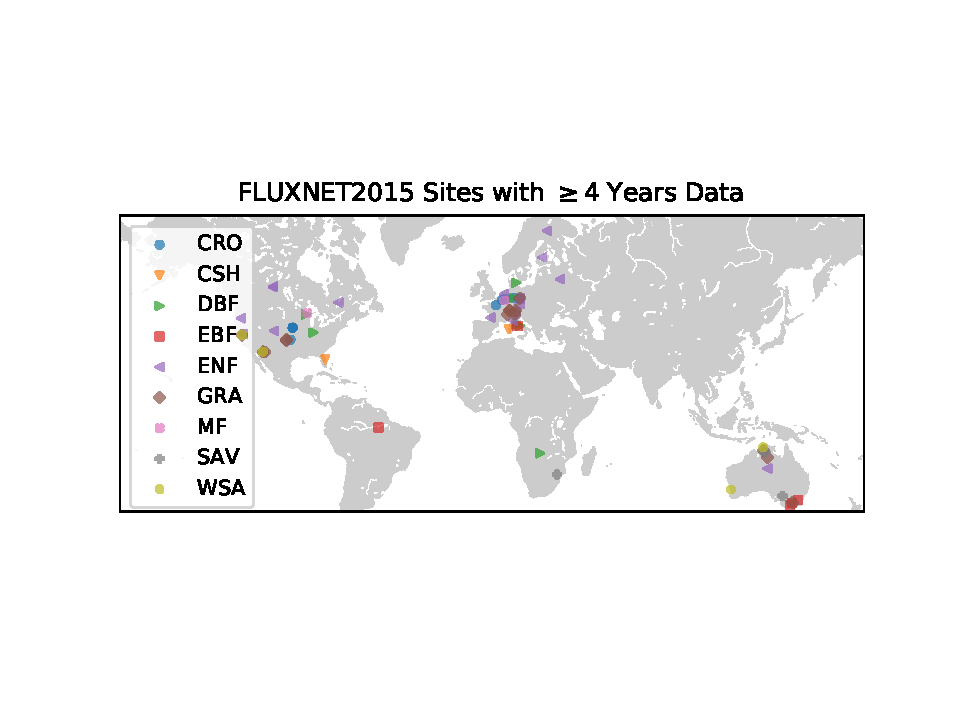
\includegraphics[trim={0 3cm 0 3cm}, clip]{./map.pdf}
  \caption{\DIFaddFL{Plant functional type and location of FLUXNET2015 sites
    used in this analysis.}}
  \label{map_fig}
\end{figure}


\DIFadd{The purpose of this study is to examine ecosystem response to
atmospheric drying, }\DIFaddend focusing on the \DIFdelbegin \DIFdel{leaf scale \mbox{%DIFAUXCMD
\citep{Rawson1977, Turner1984, Oren1999, Damour2010,
Mott2013} }%DIFAUXCMD
does not consistently or analogously include the energetic
constraints on evapotranspiration under which ecosystems operate. The
leaf-scale results agree that stomatal conductance decreases in
response to VPD \mbox{%DIFAUXCMD
\citep{Oren1999, Damour2010}}%DIFAUXCMD
, which we expect to be
true for an ecosystem as well.
However leaf scale results also
indicate that transpiration usually increases with increasing VPD in a
concave downward shape \mbox{%DIFAUXCMD
\citep[e.g.,][]{Rawson1977, Turner1984,
Mott2013}}%DIFAUXCMD
, which may not be true for ET at the
  ecosystem scale once
energetic constraints on ET are included in the
  analysis. Our
approach allows us to estimate the expected ET response to VPD at the
ecosystem scale, including the effects of surface energy balance
constraints,
and assess how ecosystem ET response to VPD deviates from
previous leaf scale analyses. }%DIFDELCMD <

%DIFDELCMD < %%%
\DIFdel{This manuscript presents the range of possible ecosystem-scale ET
responses to VPD , given parameters previously established in peer
reviewed literature. Additionally, }\DIFdelend \DIFaddbegin \DIFadd{growing season. To accomplish
this, }\DIFaddend we \DIFdelbegin \DIFdel{explore the sensitivity of the
ET-VPD relationship to
stomatal model and framework choice, highlighting the importance of: 1) future research on stomatal
conductance and ecosystem scale modeling,and 2) thoughtful selection
of photosynthesis and stomatal conductance models in more
sophisticated land surface and earth system models}\DIFdelend \DIFaddbegin \DIFadd{filter and quality control the data using a similar procedure
as \mbox{%DIFAUXCMD
\cite{Zhou_2015}}%DIFAUXCMD
:
} \begin{itemize}
\item \DIFadd{Only measured or highest (``good'') quality gapfilled data,
  according to quality control flags, are used.
}\item \DIFadd{To isolate the growing season, we only use days in which the
  average Gross Primary Productivity (GPP) exceeds 10\% of the
  observed 95th percentile of GPP for a given site. GPP is calculated
  using the nighttime respiration partitioning method.
}\item \DIFadd{We remove days with rain and the day following to avoid issues
  with rain interception and sensor saturation at high relative
  humidity (\mbox{%DIFAUXCMD
\cite{Medlyn_2017}}%DIFAUXCMD
).
} \end{itemize}
\DIFadd{Additionally, as in \mbox{%DIFAUXCMD
\citet{Lin_2018}}%DIFAUXCMD
, we restrict data to the daytime,
which is identified when downwelling shortwave radiation is greater
than 50 W m$^{-2}$ and sensible heat flux is greater than 5 W
m$^{-2}$. To reduce the chance of sensor saturation at high relative
humidity, we remove all time steps for which VPD is less than .01 kPa,
and to reduce errors at low windspeeds we remove all periods with wind
magnitudes less than 0.5 m s$^{-1}$. Timesteps with negative observed
GPP or ET are also removed, and we aggregate half hourly data to
hourly averages to reduce noise \mbox{%DIFAUXCMD
\citep{Lin_2018}}%DIFAUXCMD
. After these quality
control procedures, 400,983 upscaled hourly observations remain}\DIFaddend .

\DIFdelbegin \section{\DIFdel{Methods}}
%DIFAUXCMD
\addtocounter{section}{-1}%DIFAUXCMD
\DIFdelend \DIFaddbegin \subsection{\DIFadd{Methods}}
\DIFaddend \label{methods}
The Penman-Monteith equation \citep [hereafter PM,][]{Penman_1948,
  Monteith_1965} estimates ET as a function of observable atmospheric
variables and surface conductances:
% \begin{linenomath*}
  \begin{equation}
    \label{orig_pen}
    ET = \frac{\Delta R_{net} + g_a \rho_a c_p VPD}{\Delta + \gamma(1 + \frac{g_a}{g_s})},
  \end{equation}
% \end{linenomath*}
where $\Delta$ is the change in saturation vapor pressure with
temperature, given by Clausius-Clapeyron ($\frac{d \; e_s}{d \; T}$),
$R_{net}$ is the net radiation minus ground heat flux, $g_a$ is
aerodynamic conductance, $\rho_a$ is air density, $c_p$ is specific
heat of air at constant pressure, $\gamma$ is the psychometric
constant, and $g_s$ is the stomatal conductance (Table
\ref{definitions}).
\DIFdelbegin \DIFdel{The issue with PM is that
  $g_s$ is a function of carbon uptake, which is has a strong
  functionally relation to ET through stomatal function. Therefore,
  when PM is formulated in terms of $g_s$, it is an implicit function
  of ET itself rather than an explicit function of ET. Here we will
  derive a new form of PM in which ET is an explicit function of plant
  parameters and environmental conditions, and use it to assess the
  ecosystem scale response to VPD (by taking a partial derivative).
}\DIFdelend

\begin{table}
  \caption{Definition of symbols and variables, with citation for how
    values are calculated, if applicable.}
  \label{definitions}
  \centering \footnotesize
  \begin{tabular}{l c c c}
    \hline
    Variable & Description & Units & Citation \\
    \hline
    $e_s$  & saturation vapor pressure & Pa  & - \\
    $T$  & temperature  & K & - \\
    $P$  & pressure & Pa  & - \\
    $\Delta$  & $\frac{\partial e_s}{\partial T}$ & Pa K$^{-1}$ & - \\
    $R_{net}$  & net radiation at land surface minus ground heat flux & W m$^{-2}$   & - \\
    $g_a$  & aerodynamic conductance & m s$^{-1}$  & \citet{Shuttleworth_2012} \\
    $\rho_a$  & air density & kg m$^{-3}$  & - \\
    $c_p$  & specific heat capacity of air at constant pressure & J K$^{-1}$ kg$^{-1}$ & - \\
    $VPD$  & vapor pressure deficit & Pa  & - \\
    $\gamma$  & psychometric constant & Pa K$^{-1}$   & - \\
    \DIFaddbeginFL \DIFaddFL{$g_{s-leaf}$  }& \DIFaddFL{leaf-scale stomatal conductance }& \DIFaddFL{m s$^{-1}$  }& \DIFaddFL{\mbox{%DIFAUXCMD
\citet{MEDLYN_2011} }%DIFAUXCMD
}\\
    \DIFaddendFL $g_{s}$  &  stomatal conductance & m s$^{-1}$
                                   & \citet{Medlyn_2017} \\
    \DIFaddbeginFL \DIFaddFL{$g_{1-leaf}$  }& \DIFaddFL{leaf-scale slope parameter }& \DIFaddFL{Pa$^{0.5}$
                                   }& \DIFaddFL{\mbox{%DIFAUXCMD
\citet{MEDLYN_2011} }%DIFAUXCMD
}\\
    \DIFaddendFL $g_{1}$  & ecosystem-scale slope parameter & Pa$^{0.5}$ & \citet{Medlyn_2017} \\
    $R$ & universal gas constant & J mol$^{-1}$ K$^{-1}$ & - \\
    $R_{air}$ & gas constant of air & J  K$^{-1}$ kg$^{-1}$ & - \\
    $\sigma$ & uncertainty parameter & -& - \\
    $c_a$ & CO$_2$ concentration & $\mu$ mol CO$_2$ mol$^{-1}$ air& - \\
    \DIFdelbeginFL \DIFdelFL{$\lambda = \frac{\partial \; transpiration}{\partial\; CO_2\; assimilation}$ }\DIFdelendFL \DIFaddbeginFL \DIFaddFL{$\lambda$ }\DIFaddendFL & marginal water cost of leaf carbon & mol H$_2$O mol$^{-1}$ CO$_2$ & - \\
    $\Gamma$ & CO$_2$ compensation point & - & - \\
    $\Gamma^*$ & CO$_2$ compensation point without dark respiration & - & - \\
    \DIFdelbeginFL \DIFdelFL{GPP }%DIFDELCMD < & %%%
\DIFdelFL{gross primary production }%DIFDELCMD < & %%%
\DIFdelFL{$\mu$-mol C s$^{-1}$ m$^{-2}$ }%DIFDELCMD < & %%%
\DIFdelFL{-
    }%DIFDELCMD < \\
%DIFDELCMD <     %%%
\DIFdelFL{ET }%DIFDELCMD < & %%%
\DIFdelFL{evapotranspiration }%DIFDELCMD < & %%%
\DIFdelFL{W m$^{-2}$ }%DIFDELCMD < & %%%
\DIFdelFL{- }%DIFDELCMD < \\
%DIFDELCMD <    %%%
\DIFdelFL{uWUE }%DIFDELCMD < & %%%
\DIFdelFL{underlying water use efficiency }%DIFDELCMD < & %%%
\DIFdelFL{$\mu$-mol C Pa$^{0.5}$
                                            J$^{-1}$ ET  }%DIFDELCMD < &
%DIFDELCMD <                                                            %%%
\DIFdelFL{\mbox{%DIFAUXCMD
\citet{Zhou_2015} }%DIFAUXCMD
}%DIFDELCMD < \\
%DIFDELCMD <     %%%
\DIFdelendFL \\ \hline
  \end{tabular}
\end{table}


\citet{MEDLYN_2011} developed a model for stomatal conductance ($g_s$)
by combining an optimal photosynthesis theory \citep{Cowan_1977} with an empirical approach, which describes the
dependence of $g_s$ to VPD. \DIFdelbegin \DIFdel{They also extended this model to the ecosystem scale
\mbox{%DIFAUXCMD
\citep{Medlyn_2017}}%DIFAUXCMD
}\DIFdelend \DIFaddbegin \DIFadd{This resulted in the following model for
leaf-scale stomatal conductance}\DIFaddend :

% \begin{linenomath*}
  \begin{equation}
    g\DIFdelbegin \DIFdel{_s }\DIFdelend \DIFaddbegin \DIFadd{_{s-leaf} }\DIFaddend = \DIFdelbegin \DIFdel{\frac{R \,T}{P} \; }\DIFdelend \DIFaddbegin \DIFadd{g_0 + }\DIFaddend 1.6 \left(1 +
      \DIFdelbegin \DIFdel{\frac{g_1}{\sqrt{VPD}}}\DIFdelend \DIFaddbegin \DIFadd{\frac{g_{1-leaf}}{\sqrt{VPD}}}\DIFaddend \right) \DIFdelbegin \DIFdel{\frac{GPP}{c_a}}\DIFdelend \DIFaddbegin \DIFadd{\frac{A}{c_a}}\DIFaddend ,
    \DIFdelbegin %DIFDELCMD < %DIFDELCMD < \label{medlyn}%%%
%DIFDELCMD <   %%%
\DIFdelend \DIFaddbegin \label{leaf_medlyn}
  \DIFaddend \end{equation}
% \end{linenomath*}
\DIFdelbegin %DIFDELCMD <

%DIFDELCMD <   %%%
\DIFdel{where $g_{1}$ is a VPD }\DIFdelend \DIFaddbegin \DIFadd{where $g_{1-leaf}$ is a leaf-scale }\DIFaddend ``slope'' parameter, \DIFdelbegin \DIFdel{GPP is the ecosystem
  scale gross primary production}\DIFdelend \DIFaddbegin \DIFadd{A is the net
CO$_2$ assimilation rate}\DIFaddend , and $c_a$ is the atmospheric CO$_2$
concentration at the \DIFdelbegin \DIFdel{canopy}\DIFdelend \DIFaddbegin \DIFadd{leaf surface}\DIFaddend . \cite{MEDLYN_2011} relate the slope
parameter (\DIFdelbegin \DIFdel{$g_{1}$}\DIFdelend \DIFaddbegin \DIFadd{$g_{1-leaf}$}\DIFaddend ) to physical parameters as:
% \begin{linenomath*}
  \DIFdelbegin %DIFDELCMD <

%DIFDELCMD <   %%%
\DIFdelend \DIFaddbegin \label{slope}
  \DIFaddend \begin{equation}
    g\DIFdelbegin \DIFdel{_{1}  \propto }\DIFdelend \DIFaddbegin \DIFadd{_{1-leaf} = }\DIFaddend \sqrt{\frac{3 \, \Gamma^* \, \lambda}{1.6}},\footnote{Note this expression has units of of (mmol mol$^{-1}$)$^{1/2}$, but this can be converted to Pa$^{1/2}$ using the ideal gas law.}
  \DIFdelbegin %DIFDELCMD < %DIFDELCMD < \label{slope}%%%
%DIFDELCMD <   %%%
\DIFdelend \end{equation}
% \end{linenomath*}

where $\Gamma^*$ is the CO$_2$ compensation point for photosynthesis
(without dark respiration), and $\lambda$ is the marginal water cost
of leaf carbon
(\DIFdelbegin \DIFdel{$\frac{\partial \; \text{transpiration}}{\partial \; CO_2 assimilation}$)\mbox{%DIFAUXCMD
\citep{Farquhar_1980, Katul_2009}}%DIFAUXCMD
}\DIFdelend \DIFaddbegin \DIFadd{$\frac{\partial \; \text{transpiration}}{\partial \; A}$)}\DIFaddend . So,
\DIFdelbegin \DIFdel{$g_{1}$ }\DIFdelend \DIFaddbegin \DIFadd{$g_{1-leaf}$ }\DIFaddend is a leaf-scale term reflecting the trade-off of water for
carbon uptake. The higher \DIFdelbegin \DIFdel{$g_{1}$}\DIFdelend \DIFaddbegin \DIFadd{$g_{1-leaf}$}\DIFaddend , the more open the stomata and
the more they release water in exchange for carbon.


\DIFaddbegin \DIFadd{The Medlyn model for stomatal conductance has been shown to behave
very well across PFTs \mbox{%DIFAUXCMD
\citep[][]{Lin_2015}}%DIFAUXCMD
, and has been successfully
adopted to ecosystem scale analysis in \mbox{%DIFAUXCMD
\citet{Medlyn_2017}}%DIFAUXCMD
. In units
of m s$^{-1}$, the ecosystem scale stomatal conductance is:
}

%DIF >  \begin{linenomath*}
  \begin{equation}
    \DIFadd{g_s = \frac{R \,T}{P} \; 1.6 \left(1 + \frac{g_1}{\sqrt{VPD}}\right) \frac{GPP}{c_a},
    \label{medlyn}
  }\end{equation}
%DIF >  \end{linenomath*}

\DIFadd{where GPP is the ecosystem scale gross primary production, and $g_1$
is an ecosystem scale analogue to $g_{1-leaf}$. We solve for $g_1$
following \mbox{%DIFAUXCMD
\citet{Medlyn_2017} }%DIFAUXCMD
(Eq. (5)), and take the median $g_1$
value to be representative of each PFT (Table \ref{pft}) instead of the mean to avoid extra weighting of rare outliers.
}

\begin{table}
  \caption{\DIFaddFL{Plant functional types, their abbreviation, calculated
    Medlyn coefficient, and calculated uWUE. uWUE from
    \mbox{%DIFAUXCMD
\citet{Zhou_2015}}%DIFAUXCMD
, including the observed standard deviation, is
    shown for comparison. Note that uWUE from \mbox{%DIFAUXCMD
\citet{Zhou_2015} }%DIFAUXCMD
is
    calculated from a different set of sites, and that units are
    converted such that the quantities work with Equations 1-8 and the
    variables defined Table \ref{definitions}.}}
  \small
  \label{pft}
  \centering
  \begin{tabular}{l c c @{\qquad} c c}
    \hline
    \multirow{2}[3]{*}{Abbreviation} & \multirow{2}[3]{*}{PFT} & \multirow{2}[3]{*}{$g_1$ (Pa$^{0.5}$)} & \multicolumn{2}{c}{uWUE ($\mu$-mol [C] Pa$^{0.5}$ J$^{-1}$ [ET])}  \\
    \cmidrule{4-5}

                                     & & & \DIFaddFL{fitted }& \DIFaddFL{\mbox{%DIFAUXCMD
\citet{Zhou_2015} }%DIFAUXCMD
}\\

    \hline
    \DIFaddFL{CRO }& \DIFaddFL{Crops  }& \DIFaddFL{140.67 }& \DIFaddFL{2.85 }& \DIFaddFL{3.80 $\pm$ 1.01 }\\
\DIFaddFL{DBF }& \DIFaddFL{Deciduous Forest  }& \DIFaddFL{117.26 }& \DIFaddFL{2.96 }& \DIFaddFL{3.12 $\pm$ 0.52 }\\
\DIFaddFL{EBF }& \DIFaddFL{Evergreen Broadleaf Forest  }& \DIFaddFL{101.92 }& \DIFaddFL{3.12 }& \DIFaddFL{N/A }\\
\DIFaddFL{SAV }& \DIFaddFL{Savannah  }& \DIFaddFL{96.07 }& \DIFaddFL{2.79 }& \DIFaddFL{N/A }\\
\DIFaddFL{GRA }& \DIFaddFL{Grass  }& \DIFaddFL{145.56 }& \DIFaddFL{2.13 }& \DIFaddFL{2.68 $\pm$ 0.61 }\\
\DIFaddFL{MF }& \DIFaddFL{Mixed Forest }& \DIFaddFL{79.23 }& \DIFaddFL{3.68 }& \DIFaddFL{2.99 $\pm$ 0.62 }\\
\DIFaddFL{WSA }& \DIFaddFL{Woody Savannah  }& \DIFaddFL{117.36 }& \DIFaddFL{2.22 }& \DIFaddFL{2.88 $\pm$ 0.38 }\\
\DIFaddFL{ENF }& \DIFaddFL{Evergreen Needleleaf Forest  }& \DIFaddFL{100.54 }& \DIFaddFL{2.73 }& \DIFaddFL{3.30 $\pm$ 0.91 }\\
\DIFaddFL{CSH }& \DIFaddFL{Closed Shrub  }& \DIFaddFL{75.08 }& \DIFaddFL{2.82 }& \DIFaddFL{2.18 $\pm$ 0.44 }\\

    \hline
  \end{tabular}
\end{table}

\DIFaddend While Eq. (\DIFdelbegin \DIFdel{\ref{medlyn}}\DIFdelend \DIFaddbegin \DIFadd{3}\DIFaddend ) can be used in PM (Eq. (1)), it will make
analytical work with the function intractable because \DIFdelbegin \DIFdel{GPP }\DIFdelend \DIFaddbegin \DIFadd{$GPP$ }\DIFaddend is
functionally related to ET itself. Additionally, a perturbation to VPD
should induce a physiological plant response that will alter GPP and
cause an indirect change in stomatal conductance, in addition to the
direct effect of VPD in Eq. (\ref{medlyn}). Therefore, in order to
derive the \DIFdelbegin \DIFdel{full plant }\DIFdelend response of ET to VPD, we must account for the functional
relationship between GPP, ET, and VPD, and its effect on stomatal
conductance. We can use aforementioned semi-empirical results of
\citet{Zhou_2015} \DIFdelbegin \DIFdel{, which were inspired optimal photosynthesis
theory, }\DIFdelend as a tool to approach this
problem. \citet{Zhou_2015}, showed that  underlying Water Use
Efficiency (uWUE):

% \begin{linenomath*}
  \begin{equation}
    uWUE = \frac{GPP \cdot \sqrt{VPD}}{ET}
    \label{uwue}
  \end{equation}
% \end{linenomath*}

is relatively constant across time \DIFaddbegin \DIFadd{and moisture conditions }\DIFaddend within a
plant functional type, and correctly captures a constant relationship
between GPP, ET and VPD over a diurnal cycle \DIFdelbegin \DIFdel{during the growing season
  }\DIFdelend \citep{Zhou_2014}. The
theoretical derivation of the square root VPD dependence in \DIFdelbegin \DIFdel{uWUE }\DIFdelend \DIFaddbegin \DIFadd{$uWUE$
}\DIFaddend leverages the same assumptions used in \cite{MEDLYN_2011} to derive the
square-root VPD dependence of the stomatal conductance model (Eq.
(\ref{medlyn})).  We can use uWUE to remove the $GPP$ dependence from
$g_s$ in a way that makes PM analytically tractable:

% \begin{linenomath*}
  \begin{equation}
    g_s = \frac{R \, T}{P} 1.6 \left(1 + \frac{g_1}{\sqrt{VPD}}\right) \frac{uWUE \; ET}{c_a \; \sqrt{VPD}}.
    \label{new_g_s}
  \end{equation}
% \end{linenomath*}

Plugging Eq. (\ref{new_g_s}) into Eq. (\ref{orig_pen}) and
rearranging gives a new explicit expression for PM, in which
dependence on $GPP$ is removed:

% \begin{linenomath*}
  \begin{equation}
    ET = \frac{\Delta R_{net} + \frac{g_a\; P}{T} \left( \frac{ c_p VPD}{R_{air}} -  \frac{\gamma c_a \sqrt{VPD} }{ R \; 1.6\; \text{ uWUE } (1 + \frac{g_1}{\sqrt{VPD}})} \right) }{ \Delta + \gamma}
    \label{et}
  \end{equation}
% \end{linenomath*}

By accounting for photosynthesis changes in ecosystem conductance, with
Eq. (\ref{et}) we have \DIFdelbegin \DIFdel{used }\DIFdelend \DIFaddbegin \DIFadd{derived for the first time, using }\DIFaddend recent
results \citep[][]{MEDLYN_2011, Zhou_2014, Zhou_2015, Medlyn_2017}\DIFdelbegin \DIFdel{to derive
  }\DIFdelend \DIFaddbegin \DIFadd{, }\DIFaddend ET
explicitly as function of environmental variables and two
plant-specific constants, the slope parameter ($g_1$), and uWUE\DIFdelbegin \DIFdel{. For
  the first time we have removed the implicit dependence of ET on
  itself through the stomatal conductance term, and we have also
  replaced the added complexity of a stomatal conductance reduction
  factor and a photosynthesis model with a single parameter (uWUE). Both
  the plant parameters reflect }\DIFdelend \DIFaddbegin \DIFadd{, both
reflecting }\DIFaddend water conservation strategy. The slope parameter is related
to the willingness of stomata to trade water for CO$_2$ and to keep
stomata open\DIFdelbegin \DIFdel{(carbon cost in terms of
  water))}\DIFdelend . uWUE is a semi-empirical ecosystem-scale constant
related to how WUE changes with VPD (specifically $VPD^{-1/2}$). It is
also roughly proportional to physical constants:

\[uWUE \propto \sqrt{\frac{c_a - \Gamma}{1.6 \lambda}},\]

where $\Gamma$ is the CO$_2$ compensation point \citep[Eq. (5)
in][]{Zhou_2014}. So uWUE is related to atmospheric CO$_2$
concentration and compensation point, and is inversely proportional to
the marginal water cost of leaf carbon\DIFdelbegin \DIFdel{($\lambda$)}\DIFdelend .
\DIFdelbegin \DIFdel{This relationship
with $\lambda$ ($\propto \lambda^{-1/2}$) is important as it is the inverse of g$_1$'s
relationship with $\lambda$ ($\propto \sqrt{\lambda}$). So, uWUE
should increase as $\lambda$ decreases, and g$_1$ should decrease as $\lambda$ decreases.}\DIFdelend

\DIFdelbegin \DIFdel{With Eq. }\DIFdelend \DIFaddbegin \DIFadd{Given eddy-covariance FLUXNET2015 data (Sect. \ref{data}), every
term in our new version of PM (Eq. }\DIFaddend (\DIFdelbegin \DIFdel{\ref{et}}\DIFdelend \DIFaddbegin \DIFadd{\ref{et})) is observed, except
for uWUE, which we fit by calculating its expectation, given the model
and FLUXNET2015 data.
}

\DIFadd{However, eddy-covariance data are inherently noisy so we include a
measure of uncertainty in our analysis. To account for observational
error, as well as model uncertainty (e.g. temporal and spatial
variations of uWUE and $g_1$), we introduce an uncertainty parameter
$\sigma$ modifying uWUE:
}

%DIF >  \begin{linenomath*}
  \begin{equation}
    \DIFadd{ET = \frac{\Delta R_{net} + \frac{g_a\; P}{T} \left( \frac{ c_p VPD}{R_{air}} -  \frac{\gamma c_a \sqrt{VPD} }{ R \; 1.6\; \sigma \; \text{ uWUE } (1 + \frac{g_1}{\sqrt{VPD}})} \right) }{ \Delta + \gamma}
    \label{et_sigma}
  }\end{equation}
%DIF >  \end{linenomath*}

\DIFadd{Now, from each FLUXNET2015 observation (i.e. for each hourly
observation at every time step}\DIFaddend ) we can \DIFdelbegin \DIFdel{take the }\DIFdelend \DIFaddbegin \DIFadd{evaluate $\sigma$:
}

%DIF >  \begin{linenomath*}
  \begin{equation}
    \DIFadd{\sigma = - \frac{g_a \gamma c_a \sqrt{VPD} L_v P }{ \left(\text{ ET } ( \Delta + \gamma) - \Delta R_{net} - g_a \rho_a c_p VPD\right) 1.6 \; R\; T\; \text{ uWUE } (1 + \frac{g_1}{\sqrt{VPD}})},
    \label{sigma}
  }\end{equation}
%DIF >  \end{linenomath*}

\DIFadd{So, with this uncertainty analysis we can evaluate departure from
our theory in observations, as a departure of $\sigma$ from unity. The
variability of $\sigma$ across sites and time provides a measure of
uncertainty in our model, assumptions, as well as in the FLUXNET2015
observations themselves. The variability of $\sigma$ then propagates
 any uncertainty through to our }\DIFaddend partial derivative of \DIFdelbegin \DIFdel{ET }\DIFdelend \DIFaddbegin \DIFadd{Eq.
(\ref{et_sigma}) }\DIFaddend with respect to VPD\DIFdelbegin \DIFdel{to understand whether VPD drives or reduces ecosystem-scale ET}\DIFdelend :

% \begin{linenomath*}
  \begin{equation}
    \frac{\partial \;  ET}{\partial \; VPD} = \frac{2\; g_a \; P}{T(\Delta + \gamma)}   \left(\frac{ c_p}{R_{air}} -  \DIFdelbegin \DIFdel{\frac{\gamma c_a }{1.6 \; R\; \; \text{ uWUE }} }\DIFdelend \DIFaddbegin \DIFadd{\frac{\gamma c_a }{1.6 \; R\; \sigma \; \text{ uWUE }} }\DIFaddend \left( \frac{2 g_1 + \sqrt{VPD}}{2 (g_1 + \sqrt{VPD})^2}\right) \right)
    \DIFdelbegin \DIFdel{,
    }\DIFdelend \label{d_et}
  \end{equation}
% \end{linenomath*}

\DIFdelbegin \DIFdel{providing }\DIFdelend \DIFaddbegin \DIFadd{With Eq. (\ref{d_et}) we have an }\DIFaddend analytical framework for ecosystem
response to atmospheric demand \DIFaddbegin \DIFadd{perturbations }\DIFaddend with environmental
conditions held fixed. There are a few subtleties to taking the
derivative in Eq. (\ref{d_et}): $\Delta$ ($\frac{d e_{s}}{d T}$)
and $VPD$ are functionally related, so while taking the derivative we
evaluate
$\frac{\partial \; ET}{\partial \; VPD} = \frac{\partial \; ET}
{\partial \; e_s} \frac{\partial \; e_s}{\partial \; VPD}
\Big|_{\text{RH fixed}} + \frac{\partial \; ET}{\partial \; RH}
\frac{\partial \; RH}{\partial \; VPD} \Big|_{\text{$e_s$
    fixed}}$. $RH$ and $e_s$ are assumed to be approximately
independent, which is supported by \DIFaddbegin \DIFadd{the }\DIFaddend data (not shown).

This derivation relied either implicitly or explicitly on several
assumptions. First, we assume that VPD at the leaf surface is the same
as VPD at measurement height; physically this implies that leaves are
perfectly coupled to the atmosphere. In reality, for some conditions
and plant types the leaves can become decoupled from the boundary
layer \citep{De_2017, Medlyn_2017}. \DIFdelbegin \DIFdel{Therefore, our derivation will be most applicable in times like }\DIFdelend \DIFaddbegin \DIFadd{Given our focus on }\DIFaddend the growing
season\DIFdelbegin \DIFdel{(when we also expect uWUE to be most valid), when }\DIFdelend \DIFaddbegin \DIFadd{, which is usually characterized by }\DIFaddend relatively high insolation
\DIFdelbegin \DIFdel{induces }\DIFdelend \DIFaddbegin \DIFadd{inducing }\DIFaddend instability and convective boundary layers, \DIFdelbegin \DIFdel{and
  }\DIFdelend we would expect
the surface to be generally well coupled. An additional assumption in
the formulation of \DIFdelbegin \DIFdel{uWUE }\DIFdelend \DIFaddbegin \DIFadd{$uWUE$ }\DIFaddend \citep{Zhou_2014, Zhou_2015} and
\citet{Medlyn_2017}'s stomatal conductance model is that direct soil
evaporation \DIFaddbegin \DIFadd{(E) }\DIFaddend contributions to ET remain small relative to
transpiration \DIFdelbegin \DIFdel{. Again, this }\DIFdelend \DIFaddbegin \DIFadd{(T). This }\DIFaddend should be more true during the growing
season. The ratio of \DIFdelbegin \DIFdel{evaporation to transpiration }\DIFdelend \DIFaddbegin \DIFadd{E to T }\DIFaddend may increase immediately after rainfall
events due to high soil moisture and ponding, but VPD is generally low
anyways during these times. However, some plant types allow for
systematically larger contributions of \DIFdelbegin \DIFdel{evaporation }\DIFdelend \DIFaddbegin \DIFadd{E }\DIFaddend in ET, particularly those
with sparse canopies and smaller relative amounts of transpiration. We
therefore might expect that the theory will be most applicable to
forest PFTs, which will be most strongly coupled to the boundary layer
due to larger surface roughness, and will also generally have the
highest ratios of transpiration to evaporation. Finally, \DIFaddbegin \DIFadd{for the goal
of developing PFT-wide intuition, }\DIFaddend we assume that $g_1$ and \DIFdelbegin \DIFdel{uWUE are
constant with respect to the conceptual VPD
  perturbation}\DIFdelend \DIFaddbegin \DIFadd{$uWUE$ are
constant in space and time}\DIFaddend . Both quantities have been shown to be \DIFdelbegin \DIFdel{relatively
  constant with respect to changes in VPD \mbox{%DIFAUXCMD
\citep{Franks_2017,
    Zhou_2014}}%DIFAUXCMD
. These parameters will however vary with plant species
  and characteristics \mbox{%DIFAUXCMD
\citep[e.g. wood density, ][]{Lin_2015}}%DIFAUXCMD
, as well
  as }\DIFdelend \DIFaddbegin \DIFadd{well
conserved over space and time within a PFT relative to inter-PFT
variability. However, we would expect them to vary somewhat with
}\DIFaddend environmental conditions including \DIFaddbegin \DIFadd{very low }\DIFaddend soil water content\DIFdelbegin \DIFdel{and
  temperature\mbox{%DIFAUXCMD
\citep{Lin_2015, Manzoni2013}}%DIFAUXCMD
. Exploring possible soil
  moisture (in) dependence of the plant parameters (g$_1$ and uWUE)is
  particularly interesting because soil moisture only enters the
  partial derivative directly through these plant parameters. If the
  plant parameters are weak functions of soil moisture then the theory
  can be directly applied to a broader range of conceptual VPD
  scenarios, including observed compound events between high VPD and low soil moisture \mbox{%DIFAUXCMD
\citep{Zhou_2019}}%DIFAUXCMD
. Supplementary material for this
  manuscript explores the soil moisture dependence of }\DIFdelend \DIFaddbegin \DIFadd{,
temperature, and with intra-PFT plant-specific characteristics like
wood density for tree PFTs \mbox{%DIFAUXCMD
\citep{Lin_2015}}%DIFAUXCMD
. Given these strong
assumptions made with the goal of understanding broad, leading order
plant behaviors, we take the extra care of including and analyzing
uncertainty (Sect. \ref{testing}) and examining sensitivity to the
exponent of the VPD response (Sect. \ref{functional_form}).
}

\DIFadd{We note one final comment on our derivation which is relevant for
drought indices. If we approximate $c_a$ at a global mean CO$_2$
concentration, then the RHS of Eq. (\ref{et}) is fully defined
using commonly available weather station data and the constants
published here. This makes Eq. (\ref{et}) useful in addition to
PET in drought indices and hydrometeorological analysis for vegetated
surfaces. Equation (\ref{et}) better reflects the physics of water
exchange at the land surface and would only require fitting of uWUE
and $g_1$, and can also account for changes in CO$_2$ concentration
(assuming some relationship between $\lambda$ and }[\DIFadd{CO$_2$}]\DIFadd{), which is missing
in other drought indices such as }\DIFaddend the \DIFdelbegin \DIFdel{plant
  parameters, but excessive noise and inconsistencies preclude
  conclusions about the nature of any dependence. We provide it in
  case it is of interest to the reader, and to motivate future
  research.
}\DIFdelend \DIFaddbegin \DIFadd{Palmer Drought Severity Index
(PDSI) \mbox{%DIFAUXCMD
\citep{Swann_2016, Lemordant_2016, Lemordant_2018}}%DIFAUXCMD
. Lastly, all
code and data used in this analysis, including those used to generate
the figures and tables, are publicly available at
}\url{https://github.com/massma/climate\_et}\DIFadd{.
%DIF > \hyperref[https://github.com/massma/climate\_et]{https://github.com/massma/climate_et}.
}\DIFaddend

\DIFdelbegin \DIFdel{Because Eq. (\ref{d_et})is a partial derivative, it's utility is as a
   conceptual model for the change in ET in response to VPD with all
   other variables held fixed. This provides is a useful tool for
   identifying the effect of VPD on ET through atmospheric demand and plant response, and allows a practitioner to disentangle
   complicated feedbacks when many quantities co-vary.
However users
   of }\DIFdelend \DIFaddbegin \section{\DIFadd{Results and Discussion}}
\label{results}

\DIFadd{By construction, the variability in the $\sigma$ term (}\DIFaddend Eq.
(\DIFdelbegin \DIFdel{\ref{d_et})should take care that their interpretation
   matches the assumptions inherent in a partial derivative. For
example, results will only be as valid as the assumption that g$_1$
   and uWUE (and
by extension $\lambda$) are fixed with respect to the
   user's conceptual change in VPD. Care must also be taken with
   possible indirect effects associated with
a change in VPD: for
example, a change in ET induced by a change in VPD can cause a
   change in surface temperature, which would drive a change in net
   radiation. These types of indirect effects and
feedbacks are not
   considered in Eq.(\ref{d_et}): temperature (a variable)is
   mathematically fixed. }\DIFdelend \DIFaddbegin \DIFadd{\ref{sigma})) contains all model and observational uncertainties. For
an observation that perfectly matches our model and constant uWUE
assumption, $\sigma$ will be one. Therefore, for our assumptions and
framework to be reasonable $\sigma$ should be close to 1. An
additional concern is that $\sigma$ may in fact be correlated with
$VPD$, in which case the dependence would need to be accounted for
when taking the derivative. Fortunately, there is a very weak
dependence of $\sigma$ on VPD in their joint distribution, and
$\sigma$ is indeed close to unity i.e. $O(1)$ (Fig.
\ref{joint_vpd_sigma}). Given this weak dependence and the
distribution of $\sigma$ we have confidence in our model framework and
the data quality.
}\DIFaddend

\DIFdelbegin \subsection{\DIFdel{Framing Eq. \ref{d_et} with previous research }}
%DIFAUXCMD
\addtocounter{subsection}{-1}%DIFAUXCMD
\DIFdelend \DIFaddbegin \begin{figure}[h]
  \centering\includegraphics[width=0.75\textwidth]{./joint_vpd_sigma.pdf}
  \caption{\DIFaddFL{The joint distribution of $VPD$ and $\sigma$, with outliers
    removed (defined as lowest and highest 5\% of $\sigma$). $\sigma$
    exhibits a weak dependence on $VPD$, and $\sigma$ is $O(1)$ for
    the bulk of the observations.}}
  \label{joint_vpd_sigma}
\end{figure}
\DIFaddend

\DIFdelbegin \DIFdel{To account for both the
variability in plant parameters and
the environment, we will systematically analyze how the ET response to VPD(}\DIFdelend \DIFaddbegin \DIFadd{Before calculating the sensitivity of ET to VPD, we will consider the
functional form of }\DIFaddend Eq. (\ref{d_et})\DIFdelbegin \DIFdel{) varies. Eq. (\ref{d_et}) includes a
``sign'' termthat determines }\DIFdelend \DIFaddbegin \DIFadd{. There are two main terms: a
``scaling'' term, which modifies the magnitude but not }\DIFaddend the sign of the
\DIFdelbegin \DIFdel{response in addition
  to magnitude}\DIFdelend \DIFaddbegin \DIFadd{ET response to VPD ($\frac{\partial \; ET}{\partial \; VPD}$)}\DIFaddend :

\begin{equation}
  \DIFdelbegin %DIFDELCMD < %DIFDELCMD < \label{sign}%%%
%DIFDELCMD <   %%%
\DIFdel{\frac{c_p}{R_{air}} - \frac{\gamma c_a }{1.6 \; R\; \text{ uWUE }} }%DIFDELCMD < \left( %%%
\DIFdel{\frac{2 g_1 + \sqrt{VPD}}{2 (g_1 + \sqrt{VPD})^2}}%DIFDELCMD < \right)%%%
\DIFdelend \DIFaddbegin \DIFadd{\frac{g_a \; P}{T(\Delta + \gamma)}}\DIFaddend ,
\end{equation}

and a ``\DIFdelbegin \DIFdel{scaling'' term multiplying the ``}\DIFdelend sign'' term\DIFaddbegin \DIFadd{, which determines whether ET increases or
decreases with VPD (i.e. atmospheric demand driven or physiologically
controlled)}\DIFaddend :

\begin{equation}
  \DIFdelbegin \DIFdel{\frac{g_a \; P}{T(\Delta + \gamma)}}\DIFdelend \DIFaddbegin \label{sign}
  \DIFadd{\frac{c_p}{R_{air}} - \frac{\gamma c_a }{1.6 \; R\; \text{ uWUE }} }\left( \DIFadd{\frac{2 g_1 + \sqrt{VPD}}{2 (g_1 + \sqrt{VPD})^2}}\right)\DIFaddend .
\end{equation}
\DIFdelbegin %DIFDELCMD <

%DIFDELCMD < %%%
\DIFdel{In the ``sign term '' most of the quantities are relatively constant,
except for VPD}\DIFdelend \DIFaddbegin \DIFadd{All variables are positive, so the relative magnitude between the
first term }\DIFaddend and the \DIFdelbegin \DIFdel{plant parameters g$_1$ and uWUE. In the scaling
term , most of the terms are relatively constant with the exception of aerodynamic conductance ($g_a$) and temperature (especially its effect
through $\Delta$) . To determine the range of probable ETresponses to
VPD we will systematically vary these parameters according to Table
\ref{param_varying}, while all other
  parameters are held fixed (Table
  \ref{param_fixed}). Physical variables ($g_a$, $T$) and plant
physiological parameters (g$_1$, uWUE)are varied according to
literature-based expectations for a range of
  growing season conditions
and plant types \mbox{%DIFAUXCMD
\citep{Zhou_2015, Medlyn_2017}}%DIFAUXCMD
. Using this previous
literature we can connect the effect of varying plant parameters to specific plant types and characteristics. }\DIFdelend \DIFaddbegin \DIFadd{second term in the sign term (Eq. (\ref{sign}))
will determine whether ET increases or decreases with increasing
VPD. If the second term is larger then plant control dominates and ET
decreases with increasing VPD. However, if the first term is larger,
then atmospheric demand dominates and ET increases with increasing
VPD.
}\DIFaddend

\DIFdelbegin \DIFdel{All code and data used in this analysis, including those used to
  generate the figures and tables, are publicly available at }%DIFDELCMD < \url{https://github.com/massma/climate\_et}%%%
\DIFdel{.
%DIF < \hyperref[https://github.com/massma/climate\_et]{https://github.com/massma/climate_et}.
}\DIFdelend \DIFaddbegin \subsection{\DIFadd{Functional Form of the Sign Term}}
\label{sign_term}
\DIFadd{First, we explore the variables within the sign term to gain better
intuition on the driver of either the increase or reduction of ET with
VPD. CO$_2$ concentration ($c_a$) and the psychometric constant
($\gamma$) are relatively constant over the dataset considered here so
that the variability is dominated by $\sigma$ and $VPD$. uWUE could
vary with soil moisture but has been shown to be relatively constant
\mbox{%DIFAUXCMD
\citep{Zhou_2015}}%DIFAUXCMD
. This then means that the sign term only depends on
VPD for a given PFT and is approximately just a function of $VPD$. We
can further determine a critical threshold separating an increase from
a decrease in ET, i.e. the threshold $VPD_{crit}$ such that the
derivative vanishes $\frac{\partial \; ET}{\partial \; VPD} = 0$:
}\small
%DIF >  \begin{linenomath*}
  \begin{equation}
    \DIFadd{VPD_{crit} = \frac{R_{air}}{4 c_p} \left( \frac{\gamma c_a}{1.6\; R \;  uWUE} + \sqrt{\frac{\gamma c_a}{1.6\; R \;  uWUE}\left( \frac{\gamma c_a}{1.6\; R \;  uWUE} + 8 g_1 \frac{c_p}{R_{air}}\right)} - 4 g_1 \frac{c_p}{R_{air}} \right),
    \label{vpd_min_et}
  }\end{equation}
%DIF >  \end{linenomath*}
  \normalsize

  \DIFadd{noting that $VPD_{crit}$ mostly depends on the PFT parameters uWUE
  and $g_1$, and only varies weakly with climate as most other
  parameters related to the environment are nearly constant. The
  calculated value of $VPD_{crit}$ for each PFT is shown in Table
  \ref{vpd_crit}. For any values of $VPD$ less than $VPD_{crit}$, ET
  will decrease with increasing VPD
  ($\frac{\partial \; ET}{\partial \; VPD} < 0$), and for values of
  $VPD$ greater than $VPD_{crit}$, ET will increase with increasing
  VPD ($\frac{\partial \; ET}{\partial \; VPD} > 0$). In other words,
  ecosystems regulate and mitigate evaporative losses up to the VPD
  limit, $VPD_{crit}$, above which atmospheric demand is just too high
  to be entirely compensated by stomatal and ecosystem regulation. We
  note however that even though ET increases again above the critical
  threshold, $VPD_{crit}$, ET is still much lower than potential
  evaporation as stomata are still strongly regulating vapor fluxes to
  the atmosphere. However, even in the absence of soil pore
  evaporation ET cannot go completely to zero at high VPD, because
  stomata are still slightly open to perform some photosynthesis
  \mbox{%DIFAUXCMD
\citep{Ball_1987, Leuning_1990, MEDLYN_2011}}%DIFAUXCMD
. In addition, upward
  xylem transport is necessary to maintain phloem transport, as well
  as nutrient transport and thus carbon allocation \mbox{%DIFAUXCMD
\citep{De_2013,
    Nikinmaa_2013, Ryan_2014}}%DIFAUXCMD
.
}\DIFaddend

\begin{table}
  \caption{\DIFdelbeginFL \DIFdelFL{Variable quantities in the ET response to VPD. Each value
    is varied to determine the effect of a range }\DIFdelendFL \DIFaddbeginFL \DIFaddFL{Values }\DIFaddendFL of \DIFdelbeginFL \DIFdelFL{expected plant }\DIFdelendFL \DIFaddbeginFL \DIFaddFL{$VPD_{crit}$, where
    $\frac{\partial \; ET}{\partial \; VPD} = 0$, evaluated at PFT
    average values for $R_{air}$, $\gamma$, }\DIFaddendFL and \DIFdelbeginFL \DIFdelFL{environmental conditions on ET response to VPD}\DIFdelendFL \DIFaddbeginFL \DIFaddFL{$c_a$}\DIFaddendFL . \DIFdelbeginFL \DIFdelFL{A citation is
    }\DIFdelendFL \DIFaddbeginFL \DIFaddFL{PFT-specific
    constants ($g_1$, uWUE) are }\DIFaddendFL provided in \DIFdelbeginFL \DIFdelFL{cases where the quantities are directly derived from
    previous literature. Conceptually, min}\DIFdelendFL \DIFaddbeginFL \DIFaddFL{Table \ref{pft}}\DIFaddendFL . \DIFaddbeginFL \DIFaddFL{For
    }\DIFaddendFL values \DIFdelbeginFL \DIFdelFL{are extracted from
    literature to correspond to approximately the 15th percentile }\DIFdelendFL of \DIFdelbeginFL \DIFdelFL{observed conditions during the growing season}\DIFdelendFL \DIFaddbeginFL \DIFaddFL{$VPD$ less than $VPD_{crit}$}\DIFaddendFL ,
    \DIFdelbeginFL \DIFdelFL{med. values
    correspond to approximately the 50th percentile}\DIFdelendFL \DIFaddbeginFL \DIFaddFL{$\frac{\partial \; ET}{\partial \; VPD}$ will be negative}\DIFaddendFL , and \DIFdelbeginFL \DIFdelFL{max. }\DIFdelendFL \DIFaddbeginFL \DIFaddFL{for
    }\DIFaddendFL values \DIFdelbeginFL \DIFdelFL{correspond to approximately the 85th percentile}\DIFdelendFL \DIFaddbeginFL \DIFaddFL{of $VPD$ greater than $VPD_{crit}$,
    $\frac{\partial \; ET}{\partial \; VPD}$ will be positive}\DIFaddendFL .}
  \DIFdelbeginFL %DIFDELCMD < \label{param_varying}
%DIFDELCMD <   %%%
\DIFdelendFL \centering
  \begin{tabular}{l c c c c c}
    \hline
    \DIFdelbeginFL \DIFdelFL{Symbol }%DIFDELCMD < & %%%
\DIFdelFL{units }%DIFDELCMD < [%%%
\DIFdelFL{units in citation}%DIFDELCMD < ] %%%
\DIFdelendFL \DIFaddbeginFL \DIFaddFL{PFT }\DIFaddendFL & \DIFdelbeginFL \DIFdelFL{min  }\DIFdelendFL \DIFaddbeginFL \DIFaddFL{$R_{air}$ }\DIFaddendFL & \DIFdelbeginFL \DIFdelFL{med }\DIFdelendFL \DIFaddbeginFL \DIFaddFL{$c_a$ (ppm) }\DIFaddendFL & \DIFdelbeginFL \DIFdelFL{max
    }\DIFdelendFL \DIFaddbeginFL \DIFaddFL{$\gamma$  }\DIFaddendFL & \DIFdelbeginFL \DIFdelFL{citation  }\DIFdelendFL \DIFaddbeginFL \textbf{\DIFaddFL{$VPD_{crit}$ (Pa)}} \DIFaddendFL \\
    \hline
    \DIFdelbeginFL \DIFdelFL{g$_1$ }%DIFDELCMD < & %%%
\DIFdelFL{Pa$^{1/2}$ }%DIFDELCMD < [%%%
\DIFdelFL{kPa$^{1/2}$}%DIFDELCMD < ] %%%
\DIFdelendFL \DIFaddbeginFL \DIFaddFL{CRO }\DIFaddendFL & \DIFdelbeginFL \DIFdelFL{63.25 }%DIFDELCMD < [%%%
\DIFdelFL{2.00}%DIFDELCMD < ] %%%
\DIFdelendFL \DIFaddbeginFL \DIFaddFL{288.6 }\DIFaddendFL & \DIFdelbeginFL \DIFdelFL{126.49 }%DIFDELCMD < [%%%
\DIFdelFL{4.00}%DIFDELCMD < ] %%%
\DIFdelendFL \DIFaddbeginFL \DIFaddFL{376.1 }\DIFaddendFL & \DIFdelbeginFL \DIFdelFL{189.74 }%DIFDELCMD < [%%%
\DIFdelFL{6.00}%DIFDELCMD < ] %%%
\DIFdelendFL \DIFaddbeginFL \DIFaddFL{65.2 }\DIFaddendFL & \DIFdelbeginFL \DIFdelFL{Fig. 2, 7; \mbox{%DIFAUXCMD
\citet{Medlyn_2017} }%DIFAUXCMD
}\DIFdelendFL \DIFaddbeginFL \textbf{\DIFaddFL{812.8}}  \DIFaddendFL \\
\DIFdelbeginFL \DIFdelFL{uWUE }%DIFDELCMD < & %%%
\DIFdelFL{$\mu$-mol C Pa$^{0.5}$ J$^{-1}$ ET }%DIFDELCMD < [%%%
\DIFdelFL{g C hPa$^{1/2}$ kg$^{-1}$ H$_2$O}%DIFDELCMD < ] %%%
\DIFdelendFL \DIFaddbeginFL \DIFaddFL{DBF }\DIFaddendFL & \DIFdelbeginFL \DIFdelFL{2.33 }%DIFDELCMD < [%%%
\DIFdelFL{6.99}%DIFDELCMD < ] %%%
\DIFdelendFL \DIFaddbeginFL \DIFaddFL{288.7 }\DIFaddendFL & \DIFdelbeginFL \DIFdelFL{3.17 }%DIFDELCMD < [%%%
\DIFdelFL{9.52}%DIFDELCMD < ] %%%
\DIFdelendFL \DIFaddbeginFL \DIFaddFL{379.5 }\DIFaddendFL & \DIFdelbeginFL \DIFdelFL{4.01 }%DIFDELCMD < [%%%
\DIFdelFL{12.05}%DIFDELCMD < ] %%%
\DIFdelendFL \DIFaddbeginFL \DIFaddFL{63.3 }\DIFaddendFL & \DIFdelbeginFL \DIFdelFL{Table 4; \mbox{%DIFAUXCMD
\citet{Zhou_2015} }%DIFAUXCMD
}\DIFdelendFL \DIFaddbeginFL \textbf{\DIFaddFL{1300.0}}  \DIFaddendFL \\
\DIFdelbeginFL \DIFdelFL{T }%DIFDELCMD < & %%%
\DIFdelFL{$^o$C }\DIFdelendFL \DIFaddbeginFL \DIFaddFL{EBF }\DIFaddendFL & \DIFdelbeginFL \DIFdelFL{10.00 }\DIFdelendFL \DIFaddbeginFL \DIFaddFL{288.3 }\DIFaddendFL & \DIFdelbeginFL \DIFdelFL{20.00 }\DIFdelendFL \DIFaddbeginFL \DIFaddFL{366.4 }\DIFaddendFL & \DIFdelbeginFL \DIFdelFL{30.00 }\DIFdelendFL \DIFaddbeginFL \DIFaddFL{61.5 }\DIFaddendFL & \DIFdelbeginFL \DIFdelFL{- }\DIFdelendFL \DIFaddbeginFL \textbf{\DIFaddFL{1130.9}}  \DIFaddendFL \\
\DIFdelbeginFL \DIFdelFL{g$_a$ }%DIFDELCMD < & %%%
\DIFdelFL{m/s }\DIFdelendFL \DIFaddbeginFL \DIFaddFL{SAV }\DIFaddendFL & \DIFdelbeginFL \DIFdelFL{0.015 }\DIFdelendFL \DIFaddbeginFL \DIFaddFL{288.8 }\DIFaddendFL & \DIFdelbeginFL \DIFdelFL{0.035 }\DIFdelendFL \DIFaddbeginFL \DIFaddFL{374.2 }\DIFaddendFL & \DIFdelbeginFL \DIFdelFL{0.055 }\DIFdelendFL \DIFaddbeginFL \DIFaddFL{66.6 }\DIFaddendFL & \DIFdelbeginFL \DIFdelFL{- }\DIFdelendFL \DIFaddbeginFL \textbf{\DIFaddFL{3502.6}}  \DIFaddendFL \\
\DIFdelbeginFL %DIFDELCMD <

%DIFDELCMD <     \hline
%DIFDELCMD <   \end{tabular}
%DIFDELCMD < \end{table}
%DIFDELCMD <

%DIFDELCMD < \begin{table}
%DIFDELCMD <   %%%
%DIFDELCMD < \caption{%
{%DIFAUXCMD
\DIFdelFL{Quantities that are fixed in the ET response to VPD
    (relative to those in Table \ref{param_varying}).}}
  %DIFAUXCMD
%DIFDELCMD < \label{param_fixed}
%DIFDELCMD <   \centering
%DIFDELCMD <   \begin{tabular}{l c c}
%DIFDELCMD <     \hline
%DIFDELCMD <     %%%
\DIFdelFL{Symbol }\DIFdelendFL \DIFaddbeginFL \DIFaddFL{GRA }\DIFaddendFL & \DIFdelbeginFL \DIFdelFL{units }\DIFdelendFL \DIFaddbeginFL \DIFaddFL{288.4 }\DIFaddendFL & \DIFdelbeginFL \DIFdelFL{value }\DIFdelendFL \DIFaddbeginFL \DIFaddFL{379.1 }& \DIFaddFL{60.6 }& \textbf{\DIFaddFL{2943.6}}  \DIFaddendFL \\
\DIFdelbeginFL %DIFDELCMD < \hline
%DIFDELCMD <     %%%
\DIFdelFL{P }\DIFdelendFL \DIFaddbeginFL \DIFaddFL{MF }\DIFaddendFL & \DIFdelbeginFL \DIFdelFL{Pa }\DIFdelendFL \DIFaddbeginFL \DIFaddFL{288.2 }\DIFaddendFL & \DIFdelbeginFL \DIFdelFL{100000.00 }\DIFdelendFL \DIFaddbeginFL \DIFaddFL{384.1 }& \DIFaddFL{63.5 }& \textbf{\DIFaddFL{1530.1}}  \DIFaddendFL \\
\DIFdelbeginFL \DIFdelFL{$\gamma$ }\DIFdelendFL \DIFaddbeginFL \DIFaddFL{WSA }\DIFaddendFL & \DIFdelbeginFL \DIFdelFL{Pa K$^{-1}$ }\DIFdelendFL \DIFaddbeginFL \DIFaddFL{288.4 }\DIFaddendFL & \DIFdelbeginFL \DIFdelFL{64.50 }\DIFdelendFL \DIFaddbeginFL \DIFaddFL{376.0 }& \DIFaddFL{64.6 }& \textbf{\DIFaddFL{5234.9}}  \DIFaddendFL \\
\DIFdelbeginFL \DIFdelFL{R$_{air}$ }\DIFdelendFL \DIFaddbeginFL \DIFaddFL{ENF }\DIFaddendFL & \DIFdelbeginFL \DIFdelFL{J  K$^{-1}$ kg$^{-1}$ }\DIFdelendFL \DIFaddbeginFL \DIFaddFL{288.1 }\DIFaddendFL & \DIFdelbeginFL \DIFdelFL{288.00 }\DIFdelendFL \DIFaddbeginFL \DIFaddFL{379.2 }& \DIFaddFL{60.5 }& \textbf{\DIFaddFL{2443.6}}  \DIFaddendFL \\
\DIFdelbeginFL \DIFdelFL{c$_a$ }\DIFdelendFL \DIFaddbeginFL \DIFaddFL{CSH }\DIFaddendFL & \DIFdelbeginFL \DIFdelFL{$\mu$ mol CO$_2$ mol$^{-1}$ air }\DIFdelendFL \DIFaddbeginFL \DIFaddFL{289.0 }\DIFaddendFL & \DIFdelbeginFL \DIFdelFL{400.00 }\DIFdelendFL \DIFaddbeginFL \DIFaddFL{383.6 }& \DIFaddFL{67.5 }& \textbf{\DIFaddFL{5399.0}}  \DIFaddendFL \\

    \hline
  \end{tabular}
  \DIFaddbeginFL \label{vpd_crit}
\DIFaddendFL \end{table}


\DIFdelbegin \section{\DIFdel{Results}}
%DIFAUXCMD
\addtocounter{section}{-1}%DIFAUXCMD
%DIFDELCMD < %DIFDELCMD < \label{results}%%%
%DIFDELCMD < %%%
\DIFdelend \DIFaddbegin \DIFadd{Differences in $VPD_{crit}$ are exclusively determined by uWUE and the
slope parameter ($g_1$) related to the plant functional type. A larger
uWUE means a smaller $VPD_{crit}$, and an ET response to increases VPD
that is more likely to be positive. At first glance this result is
somewhat counter-intuitive; we expect that plants with a higher water
use efficiency would be more water conservative. However, in reality
uWUE determines how $WUE$ changes with VPD:
}\DIFaddend

\DIFdelbegin \DIFdel{By varying four parameters (g$_a$, T, uWUE , g$_1$) at three different
values (Table \ref{param_varying}) we generate nine different values
for the scaling term, nine different curves (as a function of VPD) for
the sign term, and 81 different curves for the
}\DIFdelend \DIFaddbegin \[\DIFadd{WUE = \frac{GPP}{ET} = \frac{uWUE}{\sqrt{VPD}}.}\]
\[\DIFadd{\frac{\partial \; WUE}{\partial \; VPD} = -\frac{uWUE}{2 \;
    VPD^{3/2}}}\]

\DIFadd{So, plants with a higher uWUE will have a greater }\textit{\DIFadd{decrease}} \DIFadd{in
ecosystem-scale $WUE$ in response to increases in VPD. This decrease
in $WUE$ causes more water loss per unit carbon gain, and explains the
relationship between high uWUE and high likelihood of increases of ET
in response to increasing atmospheric drying (increases in VPD).
}

\DIFadd{A tendency towards increasing ET response with increasing VPD can also
be caused by a high slope parameter ($g_1$), characteristic of plants
that at the leaf scale are more willing to trade water for access to
atmospheric CO$_2$. Plants that are less conservative will be thus be
more likely to increase ET with increasing VPD. Both the
aforementioned effects (large uWUE, $g_1$) can amplify each other, and
generally conspire to shift the sign term towards a positive value for
a given PFT.
}

\DIFadd{This effect of uWUE and $g1$ on the sign term is most apparent by
comparing two extreme PFTs: water intensive crops (CRO) and water
conservative closed shrub (CSH). CRO has higher slope parameter and a
slightly higher uWUE ($g_1 = 140.7$ Pa$^{1/2}$; $2.85$ $\mu$-mol }[\DIFadd{C}]
\DIFadd{Pa$^{0.5}$ J$^{-1}$ }[\DIFaddend ET\DIFdelbegin \DIFdel{response to VPD
($\frac{\partial \; ET}{\partial \; VPD}$).
To aid visualization we
can examine a subset of nine of these 81 curves, defined by the minimum, median and
maximum values for both the scaling and sign term
(Figure \ref{full}). The range of }\DIFdelend \DIFaddbegin ]\DIFadd{) compared to CSH ($g1 = 75.1 \, Pa^{1/2}$,
$uWUE=2.82$ $\mu$-mol }[\DIFadd{C}] \DIFadd{Pa$^{0.5}$ J$^{-1}$ }[\DIFadd{ET}]\DIFadd{). These differences
in PFT parameters cause opposite }\DIFaddend ET responses to \DIFdelbegin \DIFdel{VPD vary from those
where ET almost }\DIFdelend \DIFaddbegin \DIFadd{changes in VPD
between CRO and CSH. ET theoretically }\DIFaddend always decreases with increasing
VPD \DIFdelbegin \DIFdel{(water conservative ), to those where ET almost always }\DIFdelend \DIFaddbegin \DIFadd{for the more water conservative CSH, while ET frequently }\DIFaddend increases
with increasing VPD \DIFdelbegin \DIFdel{(water intensive ). Additionally, for some parameters
whether ET will increase or decrease with increasing VPDdepends on
atmospheric demand (Figure \ref{full})}\DIFdelend \DIFaddbegin \DIFadd{for the more water intensive CRO (Fig.
\ref{idealized_sign}). CROs evolved or were bred to prioritize GPP and
yield and are thus not water conservative. They are very willing to
trade water for photosynthesis and productivity, despite changes in
VPD, while CSH are very unwilling to trade water for more
photosynthesis}\DIFaddend .

\begin{figure}
  \centering \DIFdelbeginFL %DIFDELCMD < \includegraphics{./fully_idealized.pdf}
%DIFDELCMD <   %%%
\DIFdelendFL \DIFaddbeginFL \includegraphics{./idealized_sign.pdf}
  \DIFaddendFL \caption{The functional form of \DIFdelbeginFL \DIFdelFL{$\frac{\partial \; ET}{\partial
      \; VPD}$ for minimum}\DIFdelendFL \DIFaddbeginFL \DIFaddFL{the sign term, with $\sigma$ held
    fixed at 1}\DIFaddendFL , \DIFdelbeginFL \DIFdelFL{median }\DIFdelendFL and \DIFdelbeginFL \DIFdelFL{maximum values }\DIFdelendFL \DIFaddbeginFL \DIFaddFL{all terms except VPD set to PFT averages. For
    comparison, the observed range }\DIFaddendFL of \DIFdelbeginFL \DIFdelFL{both }\DIFdelendFL \DIFaddbeginFL \DIFaddFL{VPD for each PFT is plotted
    below }\DIFaddendFL the \DIFdelbeginFL \DIFdelFL{sign
    term }\DIFdelendFL \DIFaddbeginFL \DIFaddFL{x-axis. Stars denote 25th, 50th, and 75th percentiles,
    }\DIFaddendFL and the \DIFdelbeginFL \DIFdelFL{scaling term}\DIFdelendFL \DIFaddbeginFL \DIFaddFL{range of the line spans the 5th-95th percentiles of
    observed VPD. Vertical black lines denote the location of
    $VPD_{crit}$ for each PFT, with the exception of CSH and WSA, for which
    $VPD_{crit}$ is off-scale}\DIFaddendFL .}
  \DIFdelbeginFL %DIFDELCMD < %DIFDELCMD < \label{full}%%%
%DIFDELCMD < \end{figure}
%DIFDELCMD <

%DIFDELCMD < \begin{figure}
%DIFDELCMD <   \centering \includegraphics{./fully_idealized_sign.pdf}
%DIFDELCMD <   %%%
%DIFDELCMD < \caption{%
{%DIFAUXCMD
\DIFdelFL{The functional form of $\frac{\partial \; ET}{\partial
      \; VPD}$ evaluated at the median value of the scaling term, for
    varying values of g$_1$ and uWUE as given in Table \ref{param_varying}.}}
  %DIFAUXCMD
%DIFDELCMD < %DIFDELCMD < \label{sign}%%%
%DIFDELCMD < %%%
\DIFdelendFL \DIFaddbeginFL \label{idealized_sign}
\DIFaddendFL \end{figure}


\DIFdelbegin \DIFdel{Examining the sign term independent of
the scaling term illuminates
the role of the two plant parameters, g$_1$ and uWUE, in determining
the degree to which the response is water conservative
($\frac{\partial \; ET}{\partial \; VPD} < 0$) or water intensive
($\frac{\partial \; ET}{\partial \; VPD} > 0$) (Figure \ref{sign}).
Higher g$_1$ and
uWUE shift the curve towards increasing ET responses with VPD (water intensive),
}\DIFdelend \DIFaddbegin \DIFadd{As expected, the slope parameter ($g_1$) is a primary determinant of
the VPD dependence for the sign term shown in Fig.
\ref{idealized_sign}. Plants that are more conservative (small $g_1$)
will tend to reduce ET with increasing VPD, }\DIFaddend and \DIFdelbegin \DIFdel{smaller g$_1$ values lead to a higher non-linear }\DIFdelend \DIFaddbegin \DIFadd{will be very effective
at reducing ET, especially at low VPD. However, at very high VPD,
gradients in vapor pressure at the leaf scale will become very strong
as stomata reach their limits of closure in response to VPD
(parameterized with $g_1$). As a result, ET response will begin to
asymptote towards a constant ecosystem-scale values as leaf-scale
response to VPD asymptotes towards zero.  Therefore, plants with a low
$g_1$ will have the largest VPD dependence of ET response because the
difference in ET response at low VPD (leaf stomatal response
dominates) and high VPD (VPD gradient dominates) is largest. This is
apparent in the strong VPD dependence of CSH, which has the lowest
slope parameter ($g_1=75.1$ Pa$^{1/2}$) (Fig. \ref{idealized_sign}).
}

\DIFadd{To summarize our theoretical insights (Fig. \ref{idealized_sign} and
Table \ref{vpd_crit}), CROs are the least water conservative and have
the strongest overall tendency to increase ET with increasing VPD,
while CSH are the most water conservative and have the strongest
tendency to decrease ET with increasing VPD, as well as the strongest
}\DIFaddend VPD dependence of \DIFdelbegin \DIFdel{the response. However care
should be exercised when interpreting the range of ET responses, because g$_1$ and uWUE should generally be anti-correlated due to
their dependencies on $\lambda$. As $\lambda$ increases, g$_1$ should
increase and uWUE should decrease. Because high and low values of uWUE
and g$_1$ were
determined independently from each other in
previous literature, plant types with anomalously high
or low values
for }\textit{\DIFdel{both}} %DIFAUXCMD
\DIFdel{g$_1$ and uWUE should be relatively rare}\DIFdelend \DIFaddbegin \DIFadd{response. Fig. \ref{idealized_sign} clearly shows,
according to our theory, that for all PFTs except for crops there is
frequent occurrence of a negative (plant dominating) ET response to
increases in VPD. Therefore, plants are able in most atmospheric
conditions to reduce ET in response to increased VPD and thus to
reduce water loss. To better illustrate this, the ranges of observed
environmental VPDs at the FLUXNET sites are plotted parallel to the
x-axis. For CSH and WSA, VPD is always less than VPD$_{crit}$ (off
scale) so that the plant response dominates in typical environmental
conditions, emphasizing the water conservative strategy of those
plants. For CRO on the other hand, VPD is higher than VPD$_{crit}$ for
more than 50\% of observations, emphasizing that those plants operate
with an aggressive water usage strategy, are water intensive and were
actually engineered for photosynthesis rather than water saving. For
DBF, EBF, MF, GRA, and SAV more than half of the observed VPD are less
than VPD$_{crit}$, i.e. in conditions where plant response
dominates. SAV has a more water conservative response than the forest,
grass, and crop plan types, but still responds by increasing ET with
increasing VPD for about a quarter of observations, due to the high
aridity (VPD) of the SAV ecoclimate. It is also important to note that
for all PFTs, even when atmospheric demand dominates, ET response to
VPD is still far more negative than it would be for potential
evaporation $\partial PET/\partial VPD$, i.e. atmospheric demand only,
emphasizing that there is still a strong regulation of evaporative
flux by stomata and though the plant xylem. The sign term in the PET
case would just be a constant ($\frac{c_p}{R_{air}} \approx 3.5$),
which is far larger than any part of the curves for any PFT. Plants
are always regulating water exchange from the land surface, even when
they reach the limits of they ability to do so}\DIFaddend .

\DIFdelbegin %DIFDELCMD < \begin{figure}
%DIFDELCMD <   \centering \includegraphics{./fully_idealized_scaling.pdf}
%DIFDELCMD <   %%%
%DIFDELCMD < \caption{%
{%DIFAUXCMD
\DIFdelFL{The functional form of $\frac{\partial \; ET}{\partial
      \; VPD}$ evaluated at the median value of the sign term, for
    varying values of g$_a$ and T as given in Table \ref{param_varying}.}}
  %DIFAUXCMD
%DIFDELCMD < %DIFDELCMD < \label{scaling}%%%
%DIFDELCMD < \end{figure}
%DIFDELCMD <

%DIFDELCMD < %%%
\DIFdel{Examining the scaling term independent }\DIFdelend \DIFaddbegin \subsection{\DIFadd{Functional Form of the Scaling Term}}
\label{scale_term}
\DIFadd{While the above discussion }\DIFaddend of the sign \DIFdelbegin \DIFdel{term shows how aerodynamic conductance (communication between the
atmosphere and the
surface) and temperature (controls the efficiency of energy conversion
to
latent heat through }\DIFdelend \DIFaddbegin \DIFadd{of
$\frac{\partial \; ET}{\partial \; VPD}$ is important to answer our
question of when ET response increases or decreases with VPD,
understating the overall magnitude of the ET response is important to
soil-plant-atmosphere water budgeting. So we now more closely examine
the terms that affect how the sign term is scaled:
}

\begin{equation}
  \DIFadd{\frac{g_a \; P}{T(\Delta + \gamma)}.
}\end{equation}

\DIFadd{$\frac{P}{T}$ is an air-density term, which varies little compared to
aerodynamic conductance and Clausius-Clapeyron (}\DIFaddend $\Delta$\DIFdelbegin \DIFdel{), amplify or suppress the plant
response represented in the sign term(Figure \ref{scaling}). Both
lower temperatures and higher aerodynamic conductance lead to
amplified ET response to VPD, with the variability of aerodynamic conductance resulting in a slightly higher variability of ET response
relative to temperature}\DIFdelend \DIFaddbegin \DIFadd{). The
psychometric constant ($\gamma$) is also relatively constant, so the
scaling term should be primarily a function of aerodynamic conductance
and temperature, through the Clausius-Clapeyron relationship
$\Delta$. This is as expected, given that the aerodynamic conductance
represents the efficiency of exchange between the surface and the
atmosphere. As aerodynamic conductance increases, any plant response
will be communicated more strongly to the atmosphere (and vice-versa).
}

\DIFadd{$\Delta$'s presence in the scaling term also matches physical
intuition. $\Delta$ (and also the approximately constant $\gamma$)
control the efficiencies with which surface energy is converted to
latent and sensible heat \mbox{%DIFAUXCMD
\citep{Monteith_1965}}%DIFAUXCMD
. The functional from of
$\Delta$ will be the same across PFTs, but the temperature range may
vary slightly. In contrast, aerodynamic conductance will vary strongly
with PFT due to the importance of surface roughness for aerodynamic
conductance. So most of the differences in scaling between PFT should
be in the aerodynamic conductance term}\DIFaddend .

\DIFdelbegin \section{\DIFdel{Discussion}}
%DIFAUXCMD
\addtocounter{section}{-1}%DIFAUXCMD
%DIFDELCMD < %DIFDELCMD < \label{discussion}%%%
%DIFDELCMD < %%%
\DIFdelend \DIFaddbegin \DIFadd{The control of the scaling term variability between PFTs by
aerodynamic conductance is confirmed by data (Fig.
\ref{scale_vary}). Differences between PFT are almost entirely due to
differences in aerodynamic conductance, rather than differences in
observed temperature ranges. The scaling term for the tree PFTs (DBF,
EBF, ENF, MF) is generally about double the scaling terms for other
PFTs which have lower surface roughness and generally smaller
aerodynamic conductance (GRA, CSH, CRO). The savannah (WSA, SAV) PFT's
scaling is somewhere between GRA, CSH, and CRO, and DBF, EBF, ENF, and
MF, due to higher variability and surface roughness.
}\DIFaddend

\DIFdelbegin \DIFdel{Interpreting both the derivation and results of this manuscript hinges
on an understanding and appreciation for the usefulness of partial
derivatives for understanding the behavior of
complex systems in a
simplified framework. Our results are a conceptual tool for answering
the question, ``What is }\DIFdelend \DIFaddbegin \begin{figure}
  %DIF >  \centering
  \centerline{\includegraphics[width=1.2\textwidth]{./idealized_scale.pdf}}
  \caption{\DIFaddFL{Primary sources of variability for the scaling term, as a
    function of PFT. The 5th-95th percentile range of temperature is
    plotted at the 5th, 25th, 50th, 75th, and 95th percentiles of
    aerodynamic conductance, as observed for each PFT.}}
  \label{scale_vary}
\end{figure}

\DIFadd{Within each PFT, }\DIFaddend the \DIFaddbegin \DIFadd{scaling term variability is controlled both by
environmental temperature and aerodynamic conductance variability
(Fig. \ref{scale_vary}). While the observed variability of the
aerodynamic conductance contributes more to the scaling term
variability than temperature, the temperature contribution is
non-negligible. Specifically, the scaling term is generally larger at
low temperatures when latent heat is relatively inefficient at moving
energy away from the surface. This effect amplifies the role of
aerodynamic conductance variability at low temperatures.
}

\DIFadd{To summarize, variability between PFTs is mostly controlled by
systematic differences in aerodynamic conductance, due to differences
in surface roughness between each PFT, and possibly to a lesser extent
wind conditions. In contrast, variability within PFT is also
controlled by temperature, through Clausius-Clapeyron. But,
aerodynamic conductance variability generally impacts the scaling term
more than temperature, even within PFTs.
}

\subsection{\DIFadd{Bulk statistics of ET response to VPD}}
\label{stats_sec}

\DIFadd{In this section we consider direct observations of ET response with
eddy-covariance data, while including uncertainty with the $\sigma$
term (Sect. \ref{methods}). These observational results of ET
response (Table \ref{stats}) largely confirm our theoretical analysis, presented in the previous sections. For all PFTs, mean }\DIFaddend ET response to \DIFdelbegin \DIFdel{VPD with all
other
quantities held fixed?'' This is useful, and
we would argue is critical, for understanding complex responses when many quantities are
varying simultaneously \mbox{%DIFAUXCMD
\citep{Zhou_2019}}%DIFAUXCMD
.
If we cannot understand the contribution of one term to observed variability, independent of other
confounding factors, there is little hope of disentangling and
understanding the relative role of
many co-varying quantities in determining observed variability.Eq. (\ref{d_et})explicitly
provides an estimate of the }\DIFdelend \DIFaddbegin \DIFadd{increasing VPD
is negative. However, ET response evaluated at the average of all
variables (e.g. $\sigma$, $T$, $c_a$, $VPD$) is positive for CRO, and
negative for all other PFTs. This difference in mean ET response as
compared to the ET response at mean environmental conditions is due to
the non-linear nature of the response, in which negative responses are
generally larger magnitude than positive responses (Fig.
\ref{idealized_sign}). Therefore, both the mean ET response as well as
the ET response at mean environmental conditions matches our
expectations from the theory (Sect. \ref{sign_term}), with the
exception that CRO observations are shifted more towards a negative ET
response than we expect.
}

\begin{table}
  \caption{\DIFaddFL{Statistics of $\frac{\partial \; ET}{\partial \; VPD}$ as a
    function of PFT.}}
  \centering
  \begin{tabular}{l c c c}
    \hline
    \DIFaddFL{PFT }& \DIFaddFL{$\overline{\frac{\partial \; ET}{\partial \; VPD}}$ }& \DIFaddFL{$\frac{\partial \; ET}{\partial \; VPD}\left(\overline{env}\right)$ }& \DIFaddFL{fraction $\frac{\partial \; ET}{\partial \; VPD} < 0.$ }\\
    \hline
    \DIFaddFL{CRO }& \DIFaddFL{-0.041 }& \DIFaddFL{0.014 }& \DIFaddFL{0.513 }\\
\DIFaddFL{DBF }& \DIFaddFL{-0.110 }& \DIFaddFL{-0.017 }& \DIFaddFL{0.618 }\\
\DIFaddFL{EBF }& \DIFaddFL{-0.108 }& \DIFaddFL{-0.013 }& \DIFaddFL{0.634 }\\
\DIFaddFL{SAV }& \DIFaddFL{-0.038 }& \DIFaddFL{-0.031 }& \DIFaddFL{0.650 }\\
\DIFaddFL{GRA }& \DIFaddFL{-0.072 }& \DIFaddFL{-0.022 }& \DIFaddFL{0.690 }\\
\DIFaddFL{MF }& \DIFaddFL{-0.131 }& \DIFaddFL{-0.070 }& \DIFaddFL{0.711 }\\
\DIFaddFL{WSA }& \DIFaddFL{-0.085 }& \DIFaddFL{-0.070 }& \DIFaddFL{0.766 }\\
\DIFaddFL{ENF }& \DIFaddFL{-0.180 }& \DIFaddFL{-0.102 }& \DIFaddFL{0.776 }\\
\DIFaddFL{CSH }& \DIFaddFL{-0.250 }& \DIFaddFL{-0.183 }& \DIFaddFL{0.943 }\\

    \hline
  \end{tabular}
  \label{stats}
\end{table}

\DIFadd{Regarding the frequency of negative and positive ET response, all PFTs
exhibit a decreasing ET response with increasing VPD (physiologically
controlled, water conservative response) for the majority of
observations. The more water conservative PFTs generally exhibit
higher frequency of negative ET response, especially when one factors
in the distribution of environmental VPD (e.g. SAV and WSA grow in
more arid climates, Fig. \ref{idealized_sign}). In general the bulk
statistics match our theoretical expectations well, with the caveat
that inclusion of uncertainty shifts crops towards a slightly more
negative response to VPD, and shifts many of the other PFTs, which still
exhibit a high frequency of negative }\DIFaddend ET response to VPD, \DIFdelbegin \DIFdel{given assumptions
about ecosystem plant characteristics through the parameters g$_1$ and uWUE.
Eq. (\ref{d_et})is generic to
external environmental factors
and the timescale over which a VPDresponse acts, and has a straightforward conceptual interpretation. It provides the ET
response, given other quantities and parameters held fixed,
subject to
the assumptions outlined in Sect. \ref{methods}. So, while the plant
parameters g$_1$ and uWUE may vary with plant species and environmental conditions like soil moisture, we can still assess }\DIFdelend \DIFaddbegin \DIFadd{towards more frequent
occurrence of positive ET response than the theory and Fig.
\ref{idealized_sign} would suggest. The bulk statistics motivate a
more thorough examination of the structure of uncertainty and more
sophisticated validation of our theory's performance against
observations.
}

\subsection{\DIFadd{Validation of theory at eddy-covariance sites}}
\label{testing}
\DIFadd{We now compare more sophisticated distributions of the observed
response to our simplified theory (Sect. \ref{sign_term}). The
observed distribution of the sign term, as compared to what the theory
would predict, is provided in Fig. \ref{test_sign}. Our goal was to
capture the leading order behavior of the ET dependence on VPD. Given
the assumptions we made, and the uncertainties of flux tower
observations themselves, we expect a relatively large amount of noise
when reproducing the derivatives of ET. However, the data largely
reproduces our theoretical analysis.
}

\begin{figure}
  \centering
  \centerline{\includegraphics[width=1.2\textwidth]{./test_sign.pdf}}
  \caption{\DIFaddFL{Comparison of the sign term with model uncertainty included
    (box plots) to the sign term as calculated with simplifying
    assumptions (blue line, as in Fig. \ref{idealized_sign}). Each
    box plot corresponds to 5\% of the data, and the 5-95\% range of
    VPD is plotted.}}
  \label{test_sign}
\end{figure}

\DIFadd{This is particularly true for DBF and MF; the theory matches the
leading order behavior of the function when uncertainty is included,
and the observations match the theory with the addition of noise. The
VPD dependence, given by the slope parameter ($g_1$), follows the
median values of each bin. Perhaps most importantly, the x-intercept,
and thus VPD$_{crit}$, matches nearly exactly between the theory and
the observations. Therefore the sign of }\DIFaddend the ET response to \DIFdelbegin \DIFdel{VPD for a given ecosystem state, or for a given soil
moisture condition}\DIFdelend \DIFaddbegin \DIFadd{increases
in VPD should be well matched, subject to the unavoidable constraints
of noise, much of which comes from the observations themselves. The
uncertainty is non negligible; there are many observations in each bin
for which the the sign of observation is opposite the response
predicted by the theory, but to leading order our theory matches the
observations well}\DIFaddend .

\DIFdelbegin \DIFdel{However, given that g$_1$ and uWUE can vary, and they both have a large impact on the
ET response (Figure \ref{full}, \ref{sign})
, it is
useful to examine how these quantities vary in previous literature, framed by our results on $\frac{\partial \; ET}{\partial \; VPD}$. In
\mbox{%DIFAUXCMD
\citet{Zhou_2015} }%DIFAUXCMD
most plant types have uWUE similar to our median
value,
under which }\DIFdelend \DIFaddbegin \DIFadd{While CSH has a much different functional form of the sign term than
DBF and MF, CSH observations also match our theory to leading order,
albeit with a bit more variability as a function of VPD. Again, the
VPD dependence mostly determined from the slope parameter ($g_1$)
closely matches the medians in the observation bins. The
VPD-independent, strongly negative response is also captured. For CSH,
there is rare occurrence of observed positive ET response with VPD
($\approx 6$\%), even with uncertainty, so the sign of the
observations almost always matches }\DIFaddend the sign of the \DIFdelbegin \DIFdel{ET response depends on
VPD }\DIFdelend \DIFaddbegin \DIFadd{theory, which
states that ET response should always be negative.
}

\DIFadd{Biases between the theory and observations are similar for ENF, WSA,
CRO and SAV. At low VPD the theory and the observations match
well}\DIFaddend . However, \DIFdelbegin \DIFdel{crops, which we expect to prioritize carbon uptake over
water conservation, have a higher uWUE value closer to our maximum
value. This higher uWUE results in a higher likelihood for an
increasing ET responseto VPD, which matches intuition given that we expect crops to keep stomata open for access to carbon, at the cost of
increased water loss during high VPD . Shrubs, and to a lesser extent
grass, have an uWUE closer to
the minimum uWUE. For these plant types ,
we would then expect a decrease of ET in response
to VPD. It is important to note that, while \mbox{%DIFAUXCMD
\citet{Zhou_2015} }%DIFAUXCMD
did not examine the role of soil moisture for within plant-type variability of uWUE, }\DIFdelend \DIFaddbegin \DIFadd{at high VPD (upper 10-20\% of observations) the theory
is biased slightly towards positive response as compared to the
observations (Fig. \ref{test_sign}). For ENF this slight bias could
be explained by a negative bias in $g_1$. However, for WSA, CRO, and
SAV the observations in the highest VPD bins exhibit a downturn
towards more negative response, which cannot be captured by the
functional form of the sign term (Fig.
\ref{idealized_sign}). Therefore, to explain the observations one of
the variables in the sign term must change at extreme VPD (upper
10-20\%). The most likely candidate is $uWUE$, which we have assumed
constant to meet our goal of developing intuition for leading order
behavior, but might be expected to decrease at extremely low SWC. This extremely low SWC should be correlated with high VPD in very dry environments
through sensible heating increases \mbox{%DIFAUXCMD
\citep{Gentine_2016}}%DIFAUXCMD
. The theory
for EBF exhibits similar limitations as for ENF, WSA, and SAV, except
a larger portion of observations are biased negative as compared to
the theory ($\approx$ 35\%, Fig. \ref{test_sign}). However, in
general, and specifically for non-extreme VPD (VPD  $< \approx$70-90th
percentiles), the theory matches the observations for the tree and
savannah plant types well.
}

\DIFadd{The theory for GRA suffers from similar, but much more severe,
limitations as for CRO, WSA, and SAV. GRA observations are
characterized by a consistent trend back towards negative ET response
at higher VPD, which the functional form of our theory is incapable of
accounting for. As compared to CRO, WSA and SAV, the divergence
between the theory and the observations is far greater for GRA,
biasing 40-50\% of observations at higher VPD. In addition for the
potential for soil moisture to alter $uWUE$, there are other sources
of plant heterogeneity specific to GRA (and some extent CRO) that may
alter $uWUE$ (or $g_1$) or invalidate other assumptions made in the
methods section (Sect. \ref{methods}). We do not account for
variability in plant height and surface roughness, or differences in
C3 vs C4 photosynthesis and water strategies, which }\DIFaddend we might expect \DIFdelbegin \DIFdel{some variation, especially in extreme cases when soil
water becomes a
limiting factor (see supplementary material) .
}\DIFdelend \DIFaddbegin \DIFadd{to
vary substantially across sites, years, and season for GRA. These
deficiencies could largely explain the inability of our theory to
exactly match the observations in croplands. For example, a
superposition of sites with C3 plants (at low environmental VPD) and
C4 plants (at high environmental VPD) would explain the observed shift
back towards negative ET response at high VPD when all sites are
binned together, as in Fig. \ref{test_sign}. We hypothesize that the
theory would validate against observations much better if these
sources of variability were accounted for, at a cost of increased
complexity and analytical opacity.
}\DIFaddend


\DIFdelbegin \DIFdel{\mbox{%DIFAUXCMD
\citet{Medlyn_2017}}%DIFAUXCMD
's results did not display the robust relationship
between plant type and and
plant parameter (g$_1$) that was
demonstrated by \mbox{%DIFAUXCMD
\citet{Zhou_2015} }%DIFAUXCMD
foruWUE.
Given that there is a
robust relationship between g$_1$ and plant type in \mbox{%DIFAUXCMD
\citet{Lin_2015}}%DIFAUXCMD
, and that \mbox{%DIFAUXCMD
\citet{Zhou_2015}}%DIFAUXCMD
's ecosystem-scale results rely on the same
underlying theory as \mbox{%DIFAUXCMD
\citet{Medlyn_2017}}%DIFAUXCMD
's results, the ambiguous
results in \mbox{%DIFAUXCMD
\citet{Medlyn_2017} }%DIFAUXCMD
could be due to noise in ecosystem
scale observations, the consequences of imposing a model structure in
some of their g$_1$ estimations, or real ecosystem-scale within-plant
type variability }\DIFdelend \DIFaddbegin \DIFadd{While the above discussion shows that our theory has some limitations
when applied to some PFTs, especially for grasslands, it does well for
DBF, MF and CSH PFTs, and captures the response at non-extreme VPD
(VPD $< \approx$ 70th-90th percentiles) for
ENF, EBF, CRO, WSA, and SAV. In general, the leading order behavior
observed in the data is captured by the theory. Departures between our
theory and observations, specifically at high VPD, could be explained
and conceptualized with shifts in $g_1$ and/or $uWUE$ due to
site-specific plant type variability (e.g. more arid-adapted ecosystems
at more arid sites), or temporal variability for some environmental
conditions }\DIFaddend (e.g. \DIFdelbegin \DIFdel{multiple species impacting the relationship
within the eddy-covariance footprint). These differences between
leaf-scale behavior and ecosystem scale behavior highlight the
importance of understanding how and why slope parameters show
increased variability at the ecosystem scale, as argued by
\mbox{%DIFAUXCMD
\citet{Medlyn_2017}}%DIFAUXCMD
}\DIFdelend \DIFaddbegin \DIFadd{decreases in $uWUE$ at extremely low soil
moisture). To focus on general behavior and develop intuition for
PFT-scale response, we have ignored these sources of variability in
the present analysis}\DIFaddend . However, \DIFdelbegin \DIFdel{if we assume that there is some real
analogy between leaf scale results in \mbox{%DIFAUXCMD
\citet{Lin_2015} }%DIFAUXCMD
and ecosystem
scale behavior , and that some of the ambiguity in \mbox{%DIFAUXCMD
\citet{Medlyn_2017}
}%DIFAUXCMD
is due to model and/or }\DIFdelend \DIFaddbegin \DIFadd{any site-specific or temporal plant
functional variability that can be conceptualized with shifts to $g_1$
and $uWUE$ can be analyzed with our framework. This opens a door to future analyses in which plant behavior in anomalous conditions
can be explained and analyzed using Eq. (\ref{et}).
}

\subsection{\DIFadd{Observed ET response to VPD}}

\DIFadd{Most of the results presented so far focus on the sign term, so now we
turn to observations of ET response with the scaling term included
(Fig. \ref{data_scatter}). Until now, in the interest of developing
leading order intuition for ET response, and to be conservative in our
acknowledgment of model and }\DIFaddend observational error, \DIFdelbegin \DIFdel{then wecan use the
relationships between g$_1$ and plant characteristics defined by \mbox{%DIFAUXCMD
\citet{Lin_2015} }%DIFAUXCMD
to
frame the ET response to VPD}\DIFdelend \DIFaddbegin \DIFadd{we've considered
$\sigma$ variability to be a measure of uncertainty. An alternative
viewpoint is that $\sigma \cdot uWUE$ represents spatial and temporal
variability of uWUE, which may be expected within bounds \mbox{%DIFAUXCMD
\citep[see
Table \ref{pft}, also ][]{Zhou_2015}}%DIFAUXCMD
}\DIFaddend . This is \DIFdelbegin \DIFdel{subject
to the strong caveat thatwe still do not fully understand g$_1$
behavior at the
ecosystem scale. Extrapolating \mbox{%DIFAUXCMD
\citet{Lin_2015}}%DIFAUXCMD
's
results (e.g. Fig. 2) to the ecosystem scale would reveal the following relationships between g$_1$ and plant types:
}\DIFdelend \DIFaddbegin \DIFadd{a less conservative
view; some of the $\sigma \cdot uWUE$ variability will be due to model
and observational error, so by viewing $\sigma \cdot uWUE$ as
}\textit{\DIFadd{real}} \DIFadd{variability we run the risk of mistaking noise for
signal. However, the advantage of this viewpoint is that, from
\mbox{%DIFAUXCMD
\citet{Zhou_2014}}%DIFAUXCMD
, we have very high confidence that uWUE fit at the
hourly timescale (as we do with $\sigma \cdot uWUE$) correctly
captures the relationship between ET, GPP, and VPD, and that our form
of PM introduces minimal error with its use of uWUE.
}\DIFaddend

\DIFdelbegin %DIFDELCMD < \begin{itemize}
 \begin{itemize} %DIFAUXCMD
%DIFDELCMD <   \item %%%
\item%DIFAUXCMD
\DIFdel{C3 plants would have a generally higher g$_1$ than C4 plants,
  }%DIFDELCMD < \item %%%
\item%DIFAUXCMD
\DIFdel{Crops would have a larger g$_1$ than shrubs, grass, and angiosperm trees, which have a higher g$_1$ than gymnosperm
    trees.
  }%DIFDELCMD < \item %%%
\item%DIFAUXCMD
\DIFdel{Tropical and temperate climates would generally be
    characterized by plants with a higher g$_1$ than arctic and boreal
    climates.
}
 \end{itemize} %DIFAUXCMD
%DIFDELCMD < \end{itemize}
%DIFDELCMD < %%%
\DIFdel{For all of the above relationships, a higher g$_1$ means a higher
likelihood of a positive }\DIFdelend \DIFaddbegin \begin{figure}
  \centering
  \centerline{\includegraphics[width=1.2\textwidth]{./data_scatter.png}}
  \caption{\DIFaddFL{Scatter plots of observed
    $\frac{\partial \; ET}{\partial \; VPD}$, including $\sigma$
    variability, as a function of PFT, temperature and VPD. Please
    note differences in the colorbar scale.}}
  \label{data_scatter}
\end{figure}

\DIFadd{Therefore, with the caveat that some of the signal presented in Fig.
\ref{data_scatter} may in fact be noise, we can interpret the observed
distribution of }\DIFaddend ET response to \DIFdelbegin \DIFdel{increasing VPD(water
intensive), and a smaller VPD dependence of the ET response
.
}%DIFDELCMD <

%DIFDELCMD < %%%
\DIFdel{Our theoretical results highlight the variability of }\DIFdelend \DIFaddbegin \DIFadd{VPD. In general, the observed response
matches the intuitive theory. }\DIFaddend ET response to VPD \DIFdelbegin \DIFdel{as a function of both climate  and plant
characteristics, especially water usage strategy. Whether an
ecosystem increases or decreases ET in }\DIFdelend \DIFaddbegin \DIFadd{shifts towards
positive values as VPD increases (atmospheric demand dominating). CRO
exhibit the highest occurrence of positive ET response, and the
observations confirm that CRO are the most water intensive. CSH are
the most water conservative, with a strong negative response. DBF,
EBF, ENF, MF, SAV and WSA are also water conservative, but show some
occurrence of positive ET }\DIFaddend response to VPD\DIFdelbegin \DIFdel{will vary
depending on vegetation and climate. Generalizations about ET response
to VPDtherefore require thoughtful consideration of ecosystem
characteristics; statements such as ``ET increases with warming due to increases in
VPD'' may be false depending on the water conservation
strategy of a given ecosystem \mbox{%DIFAUXCMD
\citep{Lemordant_2018}}%DIFAUXCMD
.
}\DIFdelend \DIFaddbegin \DIFadd{, particularly at higher
observed VPD, as the theory predicts. GRA, while generally water
conservative, does not match the theory well, with increasing frequency of
}\textit{\DIFadd{negative}} \DIFadd{response at high VPD. This is as expected, given
previous discussion on how we might expect more inter-site and inter-year variability for GRA (Sect. \ref{testing}).
}\DIFaddend

\DIFdelbegin \DIFdel{Additionally, the sensitivity of }\DIFdelend \DIFaddbegin \DIFadd{Fig. \ref{data_scatter} also includes the impact of the scaling
term. For a given VPD, the magnitude of }\DIFaddend ET \DIFdelbegin \DIFdel{response to plant parameters
highlights the importance of understanding and developing stomatal
conductance models and parameters for the ecosystem scale.
In
particular, why and how g$_1$ behavior at the leaf scale is not analogous to the ecosystem scale must be understood. While the
derivation here was explicit about the assumption of
a constant g$_1$
term with respect to the VPD perturbation, many sophisticated land
surface models and earth system models employing stomatal conductance
models make similar assumptions about the stationarity of VPD slope
terms \mbox{%DIFAUXCMD
\citep{Niu_2011, Franks_2017, Rogers_2017, Lawrence_2019}}%DIFAUXCMD
. Many
models will assume a constant VPD slope term }\DIFdelend \DIFaddbegin \DIFadd{response does not vary
strongly with temperature, confirming that any impact of the scaling
term on the magnitude of the response is primarily due to changes in
aerodynamic conductance. Intuitively this is reasonable; aerodynamic
conductance will control how dominant balances at the land surface are
communicated to the boundary layer. While $\Delta$ controls the
efficiency of energy conversion to latent heat, it appears this is a
second order term, relative to $g_a$, for scaling ET response.
}

\DIFadd{As with Fig. \ref{test_sign}, Fig. \ref{data_scatter} matches our
expectation based on simplified theory. The sign term is most strongly
scaled by $g_a$, and in general the occurrence of positive ET response
increases as VPD increases. The willingness with which a given plant type
evolved to use water dictates the occurrence of positive versus
negative ET response. Water conservative ecosystems are highly effective
at mitigating the effects of atmospheric demand, and can store water
for later use by reducing ET in response to increasing VPD.
}

\subsection{\DIFadd{Limitations of theory: very dry soil moisture conditions}}
\label{swc_section}
\DIFadd{In formulating our theory with Penman Monteith, we implicitly did not
account for very dry soil moisture conditions. For the majority of
environmental conditions observed at the eddy covariance sites used
here, soil conditions were not extremely dry so that we could assume a
constant uWUE and $g_1$. We posit that ecosystems will generally
optimize to host plants living in conditions which they evolved
for. However, in extreme conditions and drought scenarios soil water
content (SWC) could become the limiting factor for ET response to VPD,
which our theory does not account for. In addition, low soil moisture
conditions themselves increase VPD through land-atmosphere feedback
\mbox{%DIFAUXCMD
\citep[][]{Bouchet_1963, Morton_1965, Brutsaert_1999, Ozdogan_2006,
  Salvucci_2013, Gentine_2016, Berg_2016}}%DIFAUXCMD
.
}

\DIFadd{Within our framework, any systematic bias due to the
failure to account for SWC's effects in very dry conditions should
manifest itself in a functional relationship between $\sigma$, our
uncertainty measure, and SWC, which is observed at the FLUXNET
sites. Examining the relationship between $\sigma$ and SWC will test
to what extent our theory breaks down in very dry soil moisture
conditions.
}

\DIFadd{If we again view $\sigma \cdot uWUE$ as, in addition to a measure of
uncertainty, a short time-scale observation of uWUE, we would expect
$\sigma \cdot uWUE$ to decrease at low SWC. If $\sigma \cdot uWUE$ is
a very strong function of SWC, then our theory should be conditioned
more strongly on well watered soil conditions. If $\sigma \cdot uWUE$
is weakly a function of SWC, then our theory is more universal and
independent of soil moisture conditions.
}

\DIFadd{Indeed, for all PFTs, there is some slight dependence of $\sigma \cdot
uWUE$ on SWC, especially at low SWC (Fig. \ref{swc_boxplot}). The
portion of observations for which our theory is biased by
SWC-limitations varies by PFT, due to the nonlinear threshold at which
soil moisture availability limits plant function. For CRO, MF and DBF,
soil water content only matters for about the lowest 5\% of observations
(each box is 5\% of observations in Fig. \ref{swc_boxplot}). And, CRO,
relative to DBF, has a very weak dependence on soil moisture, which is
reflective of the high likelihood that CRO sites are optimally irrigated
and not water stressed, suggesting that observed departures from the
theory for CRO are due to other factors }\DIFaddend (e.g. \DIFdelbegin \DIFdel{g$_1$) term within
a given plant functional type,
and research derived from these models
often does not acknowledge limitations of this assumption, or the difficulty in the literature with quantifying an ecosystem scale slope
parameter \mbox{%DIFAUXCMD
\citep{Medlyn_2017}}%DIFAUXCMD
. Given that something so fundamental as
the ET response to VPD varies strongly with g$_1$, we must invest more in understanding g$_1$'s behavior at the ecosystem scale}\DIFdelend \DIFaddbegin \DIFadd{different photosynthesis
pathways; C3/C4) than soil moisture. For ENF, EBF, SAV, and WSA,
systematic SWC-induced biases in $\sigma \cdot uWUE$ emerge in about the
lowest 20-30\% of SWC conditions, although large variability in the
SWC-$(\sigma \cdot uWUE)$ relationship hampers interpretation for
WSA. CSH presents a special case: the limited number of sites (2)
preclude comment on the exact PFT-wide relationship.
}

\DIFadd{In contrast to ENF, CRO, and DBF, for GRA the relationship between
$\sigma \cdot uWUE$ and SWC is more linear and affects a greater
portion of observations; about 60\% of observations. Clearly, for GRA
soil water frequently impacts plant function and alters ET response,
and our theory is limited for the majority of environmental
conditions. It is therefore not surprising that our theory tested
poorly against the data for GRA, relative to to the other PFTs
(Sect. \ref{testing}). For all other PFTs occurrence of soil
moisture impacts was rare enough to not manifest itself in bulk
statistics and figures.
}

\begin{figure}
  \centering
  \centerline{\includegraphics[width=1.2\textwidth]{./swc_boxplot.pdf}}
  \caption{\DIFaddFL{$\sigma \cdot uWUE$ as a function of PFT and SWC. Each box
    plot represents 5\% of all observations. Note that the highest
    10\% of SWC observations are excluded to better resolve variability in the much more narrow bins at lower SWC (e.g. SWC has long tails at high values).}}
  \label{swc_boxplot}
\end{figure}

\DIFadd{The observed dependence of $\sigma \cdot uWUE$ on SWC for GRA would
explain the deficiencies of our theory compared to the observations in
Fig. \ref{test_sign}, specifically the trend back towards
negative ET response at high VPD. Aforementioned feedbacks between
the land surface and the atmosphere, which are not accounted for due
to our focus on the one-way response of the land surface to
atmospheric conditions, would cause high VPD to be correlated with low
SWC \mbox{%DIFAUXCMD
\citep[][]{Gentine_2016, Berg_2016}}%DIFAUXCMD
. So, at high VPD observations
of low SWC are more likely, and this low SWC causes a lower uWUE
(Fig. \ref{swc_boxplot}). The lower uWUE at low SWC/high VPD then
leads to the observed downturn towards decreasing ET with increasing
VPD}\DIFaddend , and the \DIFdelbegin \DIFdel{efficacy of models using constant slope terms for ecosystem-scale
fluxes. Fortunately, our framework, }\DIFdelend \DIFaddbegin \DIFadd{deviation between our theory (based on a constant uWUE
assumption) and observations. It is also perhaps not coincidental that
the portion of $\sigma \cdot uWUE$ affected by low soil moisture
observations is similar to the portion of observations that do not
match our theory at high VPD. Indeed, this may suggest that for all PFTs
except for GRA, coupling and feedbacks between SWC, VPD and plant
function are relatively rare. Future research will explore these relatively rare feedbacks in extreme conditions, which due to analytical intractability will require more opaque numerical analysis of many more complex processes, including boundary layer growth and state and their relationship to surface layer coupling and free-tropospheric lapse rates and humidity.
}

\DIFadd{To summarize, our theory is limited by its inability to account for
soil water impacts on land surface response, and feedbacks between SWC
and VPD. Fortunately, for most PFTs SWC's effect on ET is relatively
rare ($<$30\% of observations) and does not manifest itself in the
majority of observations and bulk statistics. However for GRA, SWC decreases water use efficiency for the majority of
the observations. Soil moisture effects explain the deficiencies of
our theory in Sect. \ref{testing}, particularly for GRA. By
conceptualizing SWC effects as a change in $uWUE$ (}\DIFaddend and\DIFdelbegin \DIFdel{the new approach of using
robust ecosystem-scale ratios (uWUE)to remove the implicit dependence
of stomatal conductance on ET, is flexible enough to be applied to any
stomatal conductance model that contains a
dependence on GPP. }\DIFdelend \DIFaddbegin \DIFadd{/or $g_1$), it
will be possible for future analysis to explore the importance of soil
moisture on plant response to VPD, and feedbacks between plant
function, SWC, and VPD.
}\DIFaddend

\DIFdelbegin \DIFdel{So far we have discussed the role of different parameters in modulating the ET response. However, the form of the ET response is
imposed by our
choice of stomatal conductance model. We now examine
how the stomatal model choice, and specifically }\DIFdelend \DIFaddbegin \subsection{\DIFadd{Functional form of ET dependence on VPD and its relation
  to the VPD exponent}}
\label{functional_form}

\DIFadd{The theory described in Sect. \ref{sign_term} indicates that for a
given $uWUE$ and $g_1$, the ET dependence on VPD should be concave
upward, which is confirmed by eddy covariance data across most PFTs. In other words, there should be some local minimum in ET at a
critical VPD$_{crit}$, assuming the scaling and plant terms  (e.g. aerodynamic
conductance, $\Delta$, $g_1$ and $uWUE$) are held fixed. This result warrants further
investigation, because to our knowledge no one has derived the
theoretical ecosystem-scale relationship between ET and VPD while
controlling for other environmental conditions. In particular, from
personal communication, there is an apparent lack of consensus over
whether the shape of the ET-VPD curve should be concave upward (our
result) or concave downward in the absence of dramatic water stress. Given that understanding the ET-VPD
relationship of the one-way plant response is fundamental to
hypothesizing about any feedbacks between the land surface and the
atmosphere, we analyze why our derived ET-VPD relationship is concave
upward, particularly with respect to }\DIFaddend the exponent of \DIFdelbegin \DIFdel{the
}\DIFdelend VPD dependence in
\DIFdelbegin \DIFdel{the }\DIFdelend \DIFaddbegin \DIFadd{$uWUE$ and the Medlyn unified }\DIFaddend stomatal conductance model\DIFdelbegin \DIFdel{, can impact the
general form of the ET-VPD relationship.
}\DIFdelend \DIFaddbegin \DIFadd{.
}

\DIFaddend There is a theoretical basis for the square root VPD dependence in
both the stomatal conductance model and \DIFdelbegin \DIFdel{uWUE }\DIFdelend \DIFaddbegin \DIFadd{$uWUE$ }\DIFaddend based on the assumption
that stomata behave to maximize carbon gain while minimizing water
loss, which observations also generally support \citep{Lloyd_1991,
  MEDLYN_2011, Lin_2015, Zhou_2014, Zhou_2015, Medlyn_2017}. However,
some purely empirical results that fit the exponent of the VPD
dependence to data have shown that it may vary slightly from 1/2,
suggesting that stomata, as well as ecosystem-scale quantities based
on stomata theory, may not always function optimally \citep{Zhou_2015,
  Lin_2018}. Specifically with regards to \DIFdelbegin \DIFdel{uWUE}\DIFdelend \DIFaddbegin \DIFadd{$uWUE$}\DIFaddend , one would not expect
that this ecosystem scale WUE quantity will respond to VPD exactly
analogously to stomata. Direct soil evaporation's contributions to ET
should shift the exponent of the VPD dependence\DIFaddbegin \DIFadd{, especially at
conditions of low GPP when we would expect a systematically larger
portion of direct soil evaporation contributions to ET, because we
would also expect lower amounts of transpiration at low GPP}\DIFaddend . \citet{Zhou_2015}'s
results corroborate this: they found a mean empirically fit
exponential VPD dependence of 0.55, varying slightly from the
theoretically optimal value of of 0.5 for AmeriFlux
sites. \DIFaddbegin \DIFadd{Interpreting }\DIFaddend \citet{Lin_2018}'s results\DIFaddbegin \DIFadd{, which }\DIFaddend also show
variance in the empirical exponent of the VPD dependence \DIFdelbegin \DIFdel{in }\DIFdelend \DIFaddbegin \DIFadd{of }\DIFaddend the
stomatal conductance model, \DIFdelbegin \DIFdel{but interpretation of this variance }\DIFdelend is more difficult as \citet{Lin_2018} do
not handle \DIFdelbegin \DIFdel{the GPP}\DIFdelend \DIFaddbegin \DIFadd{GPP/A }\DIFaddend dependence of stomatal conductance in a directly
analogous manner to the optimal theory in \citet{MEDLYN_2011} and
\citet{Medlyn_2017}. Regardless, given that these recent results on
the relationship between VPD, GPP, and ET \citep{MEDLYN_2011,
  Zhou_2014, Zhou_2015, Medlyn_2017} form the backbone of our analysis
and are what allowed us to derive an explicit ET expression for the
first time (Eq. (\ref{et})), we will analyze if and how assumptions
about the exponent of the VPD dependence \DIFdelbegin \DIFdel{impact
}\DIFdelend \DIFaddbegin \DIFadd{impacts }\DIFaddend the shape of the
ET-VPD dependence. This analysis is also important to understand whether the choice of stomatal conductance model alters the fundamental behavior of the ET-VPD relationships, as many commonly used models  utilize a VPD exponent other than the 1/2 suggested by optimal theory \citep[e.g. ][ which uses an exponent of 1]{Leuning_1990}.
\DIFdelbegin \DIFdel{It is useful to understand how the choice of model
imposes the functional form of the ET-VPD relationship, given its
fundamental importance for land-atmosphere interactions.
}%DIFDELCMD <

%DIFDELCMD < %%%
\subsection{\DIFdel{Functional form of ET dependence on VPD and its relation
  to the VPD exponent}}
%DIFAUXCMD
\addtocounter{subsection}{-1}%DIFAUXCMD
%DIFDELCMD < \label{functional_form}
%DIFDELCMD <

%DIFDELCMD < %%%
\DIFdel{The results presented in Sect. \ref{results} indicates that for a
given uWUE and $g_1$, the ET dependence on VPD should be concave
upward. In other words, there should be some local minimum in ET at a
critical VPD$_{crit}$, assuming the scaling and plant terms
(e.g. aerodynamic conductance, $\Delta$, $g_1$ and uWUE) are held
fixed. This result warrants further investigation, because to our
knowledge no earlier work has derived the theoretical ecosystem-scale
relationship between ET and VPD in an energy balance framework, while
controlling for other environmental conditions. In particular there is
an apparent lack of consensus over whether the shape of the ET-VPD
curve should be concave upward (our result) or concave downward in the
absence of dramatic water stress. Given that understanding the ET-VPD
relationship of the one-way plant response is fundamental to
hypothesizing about any feedbacks between the land surface and the
atmosphere, we analyze why our derived ET-VPD relationship is concave
upward, particularly with respect to the exponent of VPD dependence in
uWUE and the Medlyn unified stomatal conductance model, as other
models and empirical results have suggested exponents varying from 1/2
\mbox{%DIFAUXCMD
\citep{Leuning_1990, Zhou_2015, Lin_2018}}%DIFAUXCMD
.
}\DIFdelend

By introducing $n$ \DIFdelbegin \DIFdel{, the exponent of VPD in uWUE, }\DIFdelend and $m$ \DIFdelbegin \DIFdel{, the exponent
of VPD in the stomatal conductance model, }\DIFdelend we can free our \DIFdelbegin \DIFdel{theory }\DIFdelend \DIFaddbegin \DIFadd{stomatal
conductance model }\DIFaddend from assumptions about VPD dependence:
% \begin{linenomath*}
  \begin{equation}
    g_s = \frac{R \, T}{P} 1.6 \left(1 + \frac{g*}{VPD^m}\right) \frac{*WUE \; ET}{c_a \; VPD^n},
    \label{m_n}
  \end{equation}
% \end{linenomath*}
where:
\[*WUE = \frac{GPP}{ET}VPD^n,\] and $g*$ is a generic slope parameter
of units $VPD^m$. To determine how the exponent $n$ and $m$ alter the
shape of the ET-VPD dependence we find the roots of the second
derivative of ET, using Eq. (\ref{m_n}) for stomatal conductance
($g_s$), with respect to VPD: \DIFdelbegin %DIFDELCMD <

%DIFDELCMD < %%%
\DIFdelend \begin{equation}
\frac{\partial^2 \; ET}{\partial \; VPD^2} = 0 \quad \forall \quad\frac{VPD^m}{g*} = \frac{m \left(m - 2 n - \sqrt{m^{2} - 4 m n + 2 m - 4 n^{2} + 4 n + 1} + 1\right)}{2 n \left(n - 1\right)} - 1.
\label{curves}
\end{equation}
 \DIFdelbegin %DIFDELCMD <

%DIFDELCMD < %%%
\DIFdelend With this
result we have defined the family of curves separating concave up from
concave down ET solutions (Fig. \ref{concave}). These curves are
only functions of the exponent of the VPD dependence and a quantity we
call non-dimensional VPD ($VPD^m/g*$). Several important
relations reveal themselves from Eq. (\ref{curves}):

\begin{figure}
  \centering
  \centerline{\includegraphics[width=0.75\textwidth]{./concave.pdf}}
  \caption{ Solutions corresponding to inflection points between
    concave up and concave down ET-VPD curves (Eq. (\ref{curves}))
    for three specific scenarios. Solutions are defined in terms of a
    non-dimensional VPD ($VPD^m/g_*$), but to aide physical
    interpretation the horizontal axis is additionally provided in terms of dimensionalized VPD assuming $m=1/2$ and
    $g_*=110\; Pa^{1/2}$ (average of all PFT $g_1$). The vertical axis
    has a different interpretation depending on the solution
    curve. For the blue line ($m$ varying), it corresponds to $m$,
    for the orange line ($n$ varying) it corresponds to $n$, and for
    the green line it corresponds to the value of both $n$ and $m$
    ($n=m$). Regions of the parameter space that correspond to
    concave up and concave down results are labeled.}
  \label{concave}
\end{figure}

 \begin{itemize}
  \item For optimal behavior (n, m = 1/2) the ET-VPD curve will be
    concave up regardless of the magnitude of the plant constants
    $g_1$ and \DIFdelbegin \DIFdel{uWUE}\DIFdelend \DIFaddbegin \DIFadd{$uWUE$}\DIFaddend . Therefore, the general concave up nature of our
    results, given an assumption of optimal behavior, is insensitive
    to plant type.
  \item For all physically possible exponents of VPD dependence ($n,
    m$), whether the solution is concave up or concave down does not
    depend on \DIFdelbegin \DIFdel{uWUE}\DIFdelend \DIFaddbegin \DIFadd{$uWUE$}\DIFaddend .
  \item In general, increasing the exponent of VPD dependence
    \DIFdelbegin \DIFdel{for
    either $uWUE*$ or $g_*$ }\DIFdelend increases the likelihood of a concave down result. Additionally, as
    the exponent of VPD dependence increases from the optimum value of
    1/2, whether the curve is concave upward or concave downward
    becomes a function of the plant specific slope parameter $g_*$,
    through non-dimensional VPD ($VPD^m/g_*$). Because the exponent of
    the VPD dependencies is capable of altering the fundamental shape
    of ET-VPD dependence, future research investment in understanding
    the exact VPD dependence of stomatal conductance, and further
    reconciliation of empirical and theoretical stomatal and
    ecosystem behavior should be prioritized.
 \end{itemize}
\DIFdelbegin %DIFDELCMD <

%DIFDELCMD < %%%
\DIFdelend While it is possible that in the future some other form of
VPD dependence is derived, at present \cite{MEDLYN_2011} and
\cite{Zhou_2014} \DIFaddbegin \DIFadd{firmly }\DIFaddend established n=m=1/2 as the most likely
candidate given current theory and empirical data. Additionally, we
argue that a concave up result matches physical intuition more than a
concave down result. Plants must maintain nutrient and sugar transport
through the phloem and xylem. To accomplish this, stomata must remain
slightly open \citep{De_2013, Nikinmaa_2013, Ryan_2014}. Furthermore,
even if complete stomatal closure were possible, cuticular water loss
and [at the ecosystem-scale] direct soil evaporation are still sources
of ET which increase with VPD, independent of stomatal
closure. Therefore, in the limit as VPD becomes large and we assume
plants are exercising all strategies to reduce ET, any further increase
in VPD should result in an increase in ET through cuticular water loss
and/or direct soil evaporation. This inevitable transition from
conditions when stomata respond strongly to VPD to conditions when
stomata response is asymptoting towards full closure would cause a
concave up ET-VPD curve, which is matched by \DIFdelbegin \DIFdel{our }\DIFdelend \DIFaddbegin \DIFadd{the }\DIFaddend theory. In short,
plant response becomes more limited as VPD increases, while
atmospheric demand monotonically increases with VPD, leading to the
 result that atmospheric demand dominates plant response when
atmospheric demand is high.

This analysis allows us to understand the theoretical shape of the ET
response to VPD with environmental conditions held
fixed. Accomplishing this with purely statistical
methods applied to flux observations would be very difficult, given
the relatively fast time scale of plant response and the
non-stationarity of [solar forced] environmental conditions over the
relatively coarse (half hourly) flux estimates (which is required to
obtain robust eddy-covariance statistics). Our results on the shape of
the ET-VPD curve with environmental conditions held
fixed can be built upon with future work examining how changes in VPD
and environmental conditions (e.g. soil water storage) feedback upon
one another. In the soil water storage example, over very long time
scales extremely high VPD perturbations coupled with no precipitation
could result in decreases in soil water storage such that water
becomes limiting. This could be represented by an extension of our
framework in which \DIFdelbegin \DIFdel{$\lambda$ }\DIFdelend \DIFaddbegin \DIFadd{uWUE }\DIFaddend is allowed to decrease with decreasing \DIFdelbegin \DIFdel{soil water, increasing uWUE and
decreasing g$_1$}\DIFdelend \DIFaddbegin \DIFadd{SWC, as
observed in Sect. \ref{swc_section}}\DIFaddend . Here, we focus our results by
\DIFdelbegin \DIFdel{framing them with
previous literature }\DIFdelend \DIFaddbegin \DIFadd{assuming constant PFT-wide conditions }\DIFaddend to build baseline intuition for
ET-VPD dependence. \DIFaddbegin \DIFadd{For most PFTs, the theory with plant function held
fixed matches the leading order behavior of the observations where
plant function varies (Sect. \ref{testing}).
}\DIFaddend


\conclusions
We derived a new form of Penman Monteith using the concept of
semi-empirical optimal stomatal regulation \citep{Lin_2015,
  MEDLYN_2011} and near constant uWUE \citep{Zhou_2015} to remove the
implicit dependence of stomatal conductance on GPP and ET. With our
new form of Penman Monteith we developed a theory for when an
ecosystem will tend to reduce or increase ET with increasing VPD,
which we \DIFdelbegin \DIFdel{framed using previous literature exploring the relationship
between plant parameters, plant types, and climate}\DIFdelend \DIFaddbegin \DIFadd{evaluated against a range of eddy-covariance data spanning
different climates and plant functional types}\DIFaddend . The goal was to \DIFdelbegin \DIFdel{understand the range of possible ET responses to VPD and develop some intuition for how the ET response may vary with plant types and
climate}\DIFdelend \DIFaddbegin \DIFadd{capture
the leading order behavior of the system to gain some intrinsic
knowledge for its behavior}\DIFaddend . This intuition can be used to disentangle
land atmosphere feedbacks in more complicated scenarios, and will aid
interpretation of observations and \DIFdelbegin \DIFdel{more }\DIFdelend sophisticated models.

\DIFdelbegin \DIFdel{ET response to VPD can vary from strongly
}\DIFdelend \DIFaddbegin \DIFadd{Our theory suggests that for a majority of environmental conditions,
plants will tend to conserve water and reduce ET with increasing
VPD. Stomatal regulation and plant physiological response strongly
regulate ET, and this regulation varies by PFT. CROs are the least
water conservative, while DBF, EBF, SAV, GRA, MF, WSA, ENF and CSH are
progressively more }\DIFaddend water conservative (\DIFdelbegin \DIFdel{ET
decreasing }\DIFdelend \DIFaddbegin \DIFadd{more likely to reduce ET }\DIFaddend in
response to increasing VPD)\DIFdelbegin \DIFdel{, to strongly water intensive
(ET increasing in }\DIFdelend \DIFaddbegin \DIFadd{. SAV and WSA exhibit positive ET }\DIFaddend response
to VPD \DIFdelbegin \DIFdel{), which is indicative of the
diversity of possible plant }\DIFdelend \DIFaddbegin \DIFadd{not necessarily because of poor }\DIFaddend water conservation strategies
\DIFdelbegin \DIFdel{. Higher uWUE
and g$_1$ values increase the likelihood of a positive ET
response ,
while decreasing temperature and increasing g$_a$ amplify the magnitude of the response. Previous literature \mbox{%DIFAUXCMD
\citep{Zhou_2015,
Lin_2015} }%DIFAUXCMD
suggests that crops, through association with
higher g$_1$
and uWUE, are more likely to exhibit a positive ET response to
VPD. Shrubs (lower uWUE), C4 plants (lower g$_1$), gymnosperm trees
(lower g$_1$) , and plants in arctic and boreal climates (lower g$_1$)
are more likely to exhibit a negative ET response to VPD. However
interpretation of g$_1$-induced variability is partially muddied by
ambiguity in applying leaf-scale estimations of g$_1$ to the ecosystem
scale \mbox{%DIFAUXCMD
\citep{Medlyn_2017}}%DIFAUXCMD
}\DIFdelend \DIFaddbegin \DIFadd{relative to other PFTs, but because of greater occurrence of high
atmospheric demand (VPD) relative to other PFTs. Observations of ET
response to VPD exhibit the same general behavior as the theory, with
ET response becoming more positive (atmospheric demand dominating) as
environmental VPD increases within a PFT, and more negative for PFTs
that are adapted to arid conditions and prioritize water conservation
over primary production}\DIFaddend .

Our paper builds \DIFaddbegin \DIFadd{important }\DIFaddend intuition for how plants respond to VPD
perturbations. We show that given optimal stomatal function and fixed
environmental conditions, the ET-VPD dependence is theoretically
concave upward, with ET increasing with increasing VPD as VPD
increases past some critical value \DIFdelbegin \DIFdel{where $\frac{\partial \;
ET}{\partial \; VPD} = 0$}\DIFdelend \DIFaddbegin \DIFadd{(Table \ref{vpd_crit})}\DIFaddend . However
future research should focus on fully understanding the \DIFdelbegin \DIFdel{functional form of
}\DIFdelend \DIFaddbegin \DIFadd{form of
stomatal }\DIFaddend VPD dependence, as this \DIFdelbegin \DIFdel{concave up }\DIFdelend result is sensitive to the exponent
of VPD dependence, which we currently believe is 1/2
\DIFdelbegin \DIFdel{for both uWUE and the stomatal
conductance model }\DIFdelend \citep{MEDLYN_2011, Zhou_2014}. Indeed, this sensitivity to the exponent of
VPD dependence is an important result itself: land surface models,
including those used in earth system models for climate forecasts,
employ different assumptions about the exponent of VPD dependence in
stomatal conductance \citep[e.g.,][]{Ball_1987, Leuning_1990,
MEDLYN_2011}, and these assumptions can fundamentally change the
relationship between ET and VPD from one that is concave upward (local
minimum in ET) to one that is concave downward (local maximum in ET).

Our results are also applicable to understanding the impact
of  expected increases in VPD
induced by global change.  Plant physiological responses to direct
CO$_2$ effects \citep[e.g.,][]{Swann_2016, Lemordant_2018} receives more attention
than physiological response to indirect effects like increased
VPD\DIFdelbegin \DIFdel{\mbox{%DIFAUXCMD
\citep{Novick_2016}}%DIFAUXCMD
}\DIFdelend . Here, we provide \DIFdelbegin \DIFdel{a framework for understanding ET response to VPD
using a simplified model of two plant parameters}\DIFdelend \DIFaddbegin \DIFadd{broad PFT-focused results showing a likely
decrease in ET in response to positive VPD perturbations (atmospheric
drying), which is consistent with recent observational analysis
\mbox{%DIFAUXCMD
\citep[e.g.,][]{Rigden_2017}}%DIFAUXCMD
}\DIFaddend . Feedbacks between the land and the
atmosphere may alter the net response to a long-timescale global VPD perturbation,
but our focus on the one way plant response to a VPD perturbation in
the atmospheric boundary layer is an important first step to
disentangling such feedbacks, both in observations and model
simulations of the present and future. By removing Penman Monteith's
dependence on implicit relationships between GPP, VPD, and ET, we
allow for explicit, accurate future analysis of plant-VPD feedbacks
in the atmospheric boundary layer (Eq. (\ref{et})). Our approach
can be extended to examine varying plant response to more nuanced
consideration of plant type and climate. Any plant physiological
heterogeneity or feedback that can be conceptualized with shifts in $g_1$
\citep[e.g.][]{Lin_2015, Medlyn_2017} and/or uWUE
\citep[e.g.][]{Zhou_2014} are representable within our framework, which
opens the door for a hierarchy of more sophisticated climate- and
plant-specific \DIFdelbegin \DIFdel{analyses }\DIFdelend \DIFaddbegin \DIFadd{analysis }\DIFaddend of ET sensitivity to environmental variables
(including VPD). We argue that such simplified conceptual frameworks
are critical tools for disentangling land-atmosphere feedbacks at
various scales, from diurnal to seasonal and beyond, and to
characterize ET response in a warmer, atmospherically drier, and
enriched CO$_2$ world.


\codedataavailability{All code and data used
in this analysis, including those used to generate the figures and
tables, are publicly available at
\url{https://github.com/massma/climate\_et}}



\DIFaddbegin \appendix

\section{\DIFadd{FLUXNET2015 sites}}\label{flux_sites}

\appendixtables   %DIF > % needs to be added in front of appendix tables

%DIF >  below taken adapted from Trevor Keenan's FLUXNET citations
%DIF >  at github.com/trevorkeenan/FLUXNET_citations
\DIFadd{Table A1: Metadata and citations for flux sites used in this analysis. All data are gathered from }\url{www.fluxdata.org}\DIFadd{, and citations are aggregated using tools available at }\url{https://github.com/trevorkeenan/FLUXNET_citations}\DIFadd{.
}\begin{longtable}{l l l l l l l}
  \hline
  \textbf{\DIFadd{Site}} &
  \textbf{\DIFadd{PFT}} &
  \textbf{\DIFadd{Lat}} &
  \textbf{\DIFadd{Lon}} &
  \textbf{\DIFadd{Clim\textsuperscript{1}}} &
  \textbf{\DIFadd{Period}} &
  \textbf{\DIFadd{References}} \\
  \hline
  \DIFadd{AT-Neu }& \DIFadd{GRA }& \DIFadd{47.1167 }& \DIFadd{11.3175 }& \DIFadd{Unk }& \DIFadd{2002-2012 }& \DIFadd{\mbox{%DIFAUXCMD
\cite{AT-Neu} }%DIFAUXCMD
}\\
\DIFadd{AU-ASM }& \DIFadd{ENF }& \DIFadd{-22.2830 }& \DIFadd{133.2490 }& \DIFadd{Unk }& \DIFadd{2010-2013 }& \DIFadd{\mbox{%DIFAUXCMD
\cite{AU-ASM} }%DIFAUXCMD
}\\
\DIFadd{AU-Cpr }& \DIFadd{SAV }& \DIFadd{-34.0021 }& \DIFadd{140.5891 }& \DIFadd{Unk }& \DIFadd{2010-2014 }& \DIFadd{\mbox{%DIFAUXCMD
\cite{AU-Cpr} }%DIFAUXCMD
}\\
\DIFadd{AU-DaP }& \DIFadd{GRA }& \DIFadd{-14.0633 }& \DIFadd{131.3181 }& \DIFadd{Aw  }& \DIFadd{2007-2013 }& \DIFadd{\mbox{%DIFAUXCMD
\cite{AU-DaP} }%DIFAUXCMD
}\\
\DIFadd{AU-DaS }& \DIFadd{SAV }& \DIFadd{-14.1593 }& \DIFadd{131.3881 }& \DIFadd{Aw  }& \DIFadd{2008-2014 }& \DIFadd{\mbox{%DIFAUXCMD
\cite{AU-DaS} }%DIFAUXCMD
}\\
\DIFadd{AU-Dry }& \DIFadd{SAV }& \DIFadd{-15.2588 }& \DIFadd{132.3706 }& \DIFadd{Unk }& \DIFadd{2008-2014 }& \DIFadd{\mbox{%DIFAUXCMD
\cite{AU-Dry} }%DIFAUXCMD
}\\
\DIFadd{AU-Gin }& \DIFadd{WSA }& \DIFadd{-31.3764 }& \DIFadd{115.7138 }& \DIFadd{Unk }& \DIFadd{2011-2014 }& \DIFadd{\mbox{%DIFAUXCMD
\cite{AU-Gin} }%DIFAUXCMD
}\\
\DIFadd{AU-How }& \DIFadd{WSA }& \DIFadd{-12.4943 }& \DIFadd{131.1523 }& \DIFadd{Aw  }& \DIFadd{2001-2014 }& \DIFadd{\mbox{%DIFAUXCMD
\cite{AU-How} }%DIFAUXCMD
}\\
\DIFadd{AU-Rig }& \DIFadd{GRA }& \DIFadd{-36.6499 }& \DIFadd{145.5759 }& \DIFadd{Unk }& \DIFadd{2011-2014 }& \DIFadd{\mbox{%DIFAUXCMD
\cite{AU-Gin} }%DIFAUXCMD
}\\
\DIFadd{AU-Stp }& \DIFadd{GRA }& \DIFadd{-17.1507 }& \DIFadd{133.3502 }& \DIFadd{Unk }& \DIFadd{2008-2014 }& \DIFadd{\mbox{%DIFAUXCMD
\cite{AU-DaP} }%DIFAUXCMD
}\\
\DIFadd{AU-Tum }& \DIFadd{EBF }& \DIFadd{-35.6566 }& \DIFadd{148.1517 }& \DIFadd{Cfb }& \DIFadd{2001-2014 }& \DIFadd{\mbox{%DIFAUXCMD
\cite{AU-Tum} }%DIFAUXCMD
}\\
\DIFadd{AU-Whr }& \DIFadd{EBF }& \DIFadd{-36.6732 }& \DIFadd{145.0294 }& \DIFadd{Unk }& \DIFadd{2011-2014 }& \DIFadd{\mbox{%DIFAUXCMD
\cite{AU-Whr} }%DIFAUXCMD
}\\
\DIFadd{AU-Wom }& \DIFadd{EBF }& \DIFadd{-37.4222 }& \DIFadd{144.0944 }& \DIFadd{Unk }& \DIFadd{2010-2012 }& \DIFadd{\mbox{%DIFAUXCMD
\cite{AU-Wom} }%DIFAUXCMD
}\\
\DIFadd{BE-Lon }& \DIFadd{CRO }& \DIFadd{50.5516 }& \DIFadd{4.7461 }& \DIFadd{Cfb }& \DIFadd{2004-2014 }& \DIFadd{\mbox{%DIFAUXCMD
\cite{BE-Lon} }%DIFAUXCMD
}\\
\DIFadd{BE-Vie }& \DIFadd{MF }& \DIFadd{50.3051 }& \DIFadd{5.9981 }& \DIFadd{Cfb }& \DIFadd{1996-2014 }& \DIFadd{\mbox{%DIFAUXCMD
\cite{BE-Vie} }%DIFAUXCMD
}\\
\DIFadd{BR-Sa3 }& \DIFadd{EBF }& \DIFadd{-3.0180 }& \DIFadd{-54.9714 }& \DIFadd{Am }& \DIFadd{2000-2004 }& \DIFadd{\mbox{%DIFAUXCMD
\cite{BR-Sa3} }%DIFAUXCMD
}\\
\DIFadd{CA-Qfo }& \DIFadd{ENF }& \DIFadd{49.6925 }& \DIFadd{-74.3421 }& \DIFadd{Dfc }& \DIFadd{2003-2010 }& \DIFadd{\mbox{%DIFAUXCMD
\cite{CA-Qfo} }%DIFAUXCMD
}\\
\DIFadd{CA-SF1 }& \DIFadd{ENF }& \DIFadd{54.4850 }& \DIFadd{-105.8176 }& \DIFadd{Dfc }& \DIFadd{2003-2006 }& \DIFadd{\mbox{%DIFAUXCMD
\cite{CA-SF1} }%DIFAUXCMD
}\\
\DIFadd{CA-SF2 }& \DIFadd{ENF }& \DIFadd{54.2539 }& \DIFadd{-105.8775 }& \DIFadd{Dfc }& \DIFadd{2001-2005 }& \DIFadd{\mbox{%DIFAUXCMD
\cite{CA-SF1} }%DIFAUXCMD
}\\
\DIFadd{CH-Cha }& \DIFadd{GRA }& \DIFadd{47.2102 }& \DIFadd{8.4104 }& \DIFadd{Unk }& \DIFadd{2005-2014 }& \DIFadd{\mbox{%DIFAUXCMD
\cite{CH-Cha} }%DIFAUXCMD
}\\
\DIFadd{CH-Dav }& \DIFadd{ENF }& \DIFadd{46.8153 }& \DIFadd{9.8559 }& \DIFadd{Unk }& \DIFadd{1997-2014 }& \DIFadd{\mbox{%DIFAUXCMD
\cite{CH-Dav} }%DIFAUXCMD
}\\
\DIFadd{CH-Fru }& \DIFadd{GRA }& \DIFadd{47.1158 }& \DIFadd{8.5378 }& \DIFadd{Unk }& \DIFadd{2005-2014 }& \DIFadd{\mbox{%DIFAUXCMD
\cite{CH-Fru} }%DIFAUXCMD
}\\
\DIFadd{DE-Geb }& \DIFadd{CRO }& \DIFadd{51.1001 }& \DIFadd{10.9143 }& \DIFadd{Unk }& \DIFadd{2001-2014 }& \DIFadd{\mbox{%DIFAUXCMD
\cite{DE-Geb} }%DIFAUXCMD
}\\
\DIFadd{DE-Gri }& \DIFadd{GRA }& \DIFadd{50.9500 }& \DIFadd{13.5126 }& \DIFadd{Cfb }& \DIFadd{2004-2014 }& \DIFadd{\mbox{%DIFAUXCMD
\cite{DE-Gri} }%DIFAUXCMD
}\\
\DIFadd{DE-Hai }& \DIFadd{DBF }& \DIFadd{51.0792 }& \DIFadd{10.4530 }& \DIFadd{Unk }& \DIFadd{2000-2012 }& \DIFadd{\mbox{%DIFAUXCMD
\cite{DE-Hai} }%DIFAUXCMD
}\\
\DIFadd{DE-Kli }& \DIFadd{CRO }& \DIFadd{50.8931 }& \DIFadd{13.5224 }& \DIFadd{Cfb }& \DIFadd{2004-2014 }& \DIFadd{\mbox{%DIFAUXCMD
\cite{DE-Gri} }%DIFAUXCMD
}\\
\DIFadd{DE-Lkb }& \DIFadd{ENF }& \DIFadd{49.0996 }& \DIFadd{13.3047 }& \DIFadd{Unk }& \DIFadd{2009-2013 }& \DIFadd{\mbox{%DIFAUXCMD
\cite{DE-Lkb} }%DIFAUXCMD
}\\
\DIFadd{DE-Obe }& \DIFadd{ENF }& \DIFadd{50.7867 }& \DIFadd{13.7213 }& \DIFadd{Cfb }& \DIFadd{2008-2014 }& {\DIFadd{\textendash}} \\
\DIFadd{DE-Seh }& \DIFadd{CRO }& \DIFadd{50.8706 }& \DIFadd{6.4497 }& \DIFadd{Unk }& \DIFadd{2007-2010 }& \DIFadd{\mbox{%DIFAUXCMD
\cite{DE-Seh} }%DIFAUXCMD
}\\
\DIFadd{DE-Tha }& \DIFadd{ENF }& \DIFadd{50.9624 }& \DIFadd{13.5652 }& \DIFadd{Cfb }& \DIFadd{1996-2014 }& \DIFadd{\mbox{%DIFAUXCMD
\cite{DE-Tha} }%DIFAUXCMD
}\\
\DIFadd{DK-Sor }& \DIFadd{DBF }& \DIFadd{55.4859 }& \DIFadd{11.6446 }& \DIFadd{Unk }& \DIFadd{1996-2014 }& \DIFadd{\mbox{%DIFAUXCMD
\cite{DK-Sor} }%DIFAUXCMD
}\\
\DIFadd{FI-Hyy }& \DIFadd{ENF }& \DIFadd{61.8474 }& \DIFadd{24.2948 }& \DIFadd{Unk }& \DIFadd{1996-2014 }& \DIFadd{\mbox{%DIFAUXCMD
\cite{FI-Hyy} }%DIFAUXCMD
}\\
\DIFadd{FI-Sod }& \DIFadd{ENF }& \DIFadd{67.3619 }& \DIFadd{26.6378 }& \DIFadd{Unk }& \DIFadd{2001-2014 }& \DIFadd{\mbox{%DIFAUXCMD
\cite{FI-Sod} }%DIFAUXCMD
}\\
\DIFadd{FR-Gri }& \DIFadd{CRO }& \DIFadd{48.8442 }& \DIFadd{1.9519 }& \DIFadd{Cfb }& \DIFadd{2004-2013 }& \DIFadd{\mbox{%DIFAUXCMD
\cite{FR-Gri} }%DIFAUXCMD
}\\
\DIFadd{FR-LBr }& \DIFadd{ENF }& \DIFadd{44.7171 }& \DIFadd{-0.7693 }& \DIFadd{Unk }& \DIFadd{1996-2008 }& \DIFadd{\mbox{%DIFAUXCMD
\cite{FR-LBr} }%DIFAUXCMD
}\\
\DIFadd{IT-Col }& \DIFadd{DBF }& \DIFadd{41.8494 }& \DIFadd{13.5881 }& \DIFadd{Unk }& \DIFadd{1996-2014 }& \DIFadd{\mbox{%DIFAUXCMD
\cite{IT-Col} }%DIFAUXCMD
}\\
\DIFadd{IT-Cpz }& \DIFadd{EBF }& \DIFadd{41.7052 }& \DIFadd{12.3761 }& \DIFadd{Unk }& \DIFadd{1997-2009 }& \DIFadd{\mbox{%DIFAUXCMD
\cite{IT-Cpz} }%DIFAUXCMD
}\\
\DIFadd{IT-Lav }& \DIFadd{ENF }& \DIFadd{45.9562 }& \DIFadd{11.2813 }& \DIFadd{Unk }& \DIFadd{2003-2014 }& \DIFadd{\mbox{%DIFAUXCMD
\cite{IT-Lav} }%DIFAUXCMD
}\\
\DIFadd{IT-MBo }& \DIFadd{GRA }& \DIFadd{46.0147 }& \DIFadd{11.0458 }& \DIFadd{Unk }& \DIFadd{2003-2013 }& \DIFadd{\mbox{%DIFAUXCMD
\cite{IT-MBo} }%DIFAUXCMD
}\\
\DIFadd{IT-Noe }& \DIFadd{CSH }& \DIFadd{40.6061 }& \DIFadd{8.1515 }& \DIFadd{Unk }& \DIFadd{2004-2014 }& \DIFadd{\mbox{%DIFAUXCMD
\cite{IT-Noe} }%DIFAUXCMD
}\\
\DIFadd{IT-Ren }& \DIFadd{ENF }& \DIFadd{46.5869 }& \DIFadd{11.4337 }& \DIFadd{Unk }& \DIFadd{1998-2013 }& \DIFadd{\mbox{%DIFAUXCMD
\cite{IT-Ren} }%DIFAUXCMD
}\\
\DIFadd{IT-Ro2 }& \DIFadd{DBF }& \DIFadd{42.3903 }& \DIFadd{11.9209 }& \DIFadd{Unk }& \DIFadd{2002-2012 }& \DIFadd{\mbox{%DIFAUXCMD
\cite{IT-Ro2} }%DIFAUXCMD
}\\
\DIFadd{IT-SRo }& \DIFadd{ENF }& \DIFadd{43.7279 }& \DIFadd{10.2844 }& \DIFadd{Unk }& \DIFadd{1999-2012 }& \DIFadd{\mbox{%DIFAUXCMD
\cite{IT-SRo} }%DIFAUXCMD
}\\
\DIFadd{IT-Tor }& \DIFadd{GRA }& \DIFadd{45.8444 }& \DIFadd{7.5781 }& \DIFadd{Unk }& \DIFadd{2008-2014 }& \DIFadd{\mbox{%DIFAUXCMD
\cite{IT-Tor} }%DIFAUXCMD
}\\
\DIFadd{NL-Loo }& \DIFadd{ENF }& \DIFadd{52.1666 }& \DIFadd{5.7436 }& \DIFadd{Unk }& \DIFadd{1996-2013 }& \DIFadd{\mbox{%DIFAUXCMD
\cite{NL-Loo} }%DIFAUXCMD
}\\
\DIFadd{RU-Fyo }& \DIFadd{ENF }& \DIFadd{56.4615 }& \DIFadd{32.9221 }& \DIFadd{Unk }& \DIFadd{1998-2014 }& \DIFadd{\mbox{%DIFAUXCMD
\cite{RU-Fyo} }%DIFAUXCMD
}\\
\DIFadd{US-AR1 }& \DIFadd{GRA }& \DIFadd{36.4267 }& \DIFadd{-99.4200 }& \DIFadd{Dsa }& \DIFadd{2009-2012 }& \DIFadd{\mbox{%DIFAUXCMD
\cite{US-AR1} }%DIFAUXCMD
}\\
\DIFadd{US-AR2 }& \DIFadd{GRA }& \DIFadd{36.6358 }& \DIFadd{-99.5975 }& \DIFadd{Dsa }& \DIFadd{2009-2012 }& \DIFadd{\mbox{%DIFAUXCMD
\cite{US-AR1} }%DIFAUXCMD
}\\
\DIFadd{US-ARM }& \DIFadd{CRO }& \DIFadd{36.6058 }& \DIFadd{-97.4888 }& \DIFadd{Cfa }& \DIFadd{2003-2012 }& \DIFadd{\mbox{%DIFAUXCMD
\cite{US-ARM} }%DIFAUXCMD
}\\
\DIFadd{US-Blo }& \DIFadd{ENF }& \DIFadd{38.8953 }& \DIFadd{-120.6328 }& \DIFadd{Csa }& \DIFadd{1997-2007 }& \DIFadd{\mbox{%DIFAUXCMD
\cite{US-Blo} }%DIFAUXCMD
}\\
\DIFadd{US-KS2 }& \DIFadd{CSH }& \DIFadd{28.6086 }& \DIFadd{-80.6715 }& \DIFadd{Cwa }& \DIFadd{2003-2006 }& \DIFadd{\mbox{%DIFAUXCMD
\cite{US-KS2} }%DIFAUXCMD
}\\
\DIFadd{US-MMS }& \DIFadd{DBF }& \DIFadd{39.3232 }& \DIFadd{-86.4131 }& \DIFadd{Cfa }& \DIFadd{1999-2014 }& \DIFadd{\mbox{%DIFAUXCMD
\cite{US-MMS} }%DIFAUXCMD
}\\
\DIFadd{US-Me2 }& \DIFadd{ENF }& \DIFadd{44.4523 }& \DIFadd{-121.5574 }& \DIFadd{Csb }& \DIFadd{2002-2014 }& \DIFadd{\mbox{%DIFAUXCMD
\cite{US-Me2} }%DIFAUXCMD
}\\
\DIFadd{US-NR1 }& \DIFadd{ENF }& \DIFadd{40.0329 }& \DIFadd{-105.5464 }& \DIFadd{Dfc }& \DIFadd{1998-2014 }& \DIFadd{\mbox{%DIFAUXCMD
\cite{US-NR1} }%DIFAUXCMD
}\\
\DIFadd{US-Ne1 }& \DIFadd{CRO }& \DIFadd{41.1651 }& \DIFadd{-96.4766 }& \DIFadd{Dfa }& \DIFadd{2001-2013 }& \DIFadd{\mbox{%DIFAUXCMD
\cite{US-Ne1} }%DIFAUXCMD
}\\
\DIFadd{US-Ne2 }& \DIFadd{CRO }& \DIFadd{41.1649 }& \DIFadd{-96.4701 }& \DIFadd{Dfa }& \DIFadd{2001-2013 }& \DIFadd{\mbox{%DIFAUXCMD
\cite{US-Ne1} }%DIFAUXCMD
}\\
\DIFadd{US-Ne3 }& \DIFadd{CRO }& \DIFadd{41.1797 }& \DIFadd{-96.4397 }& \DIFadd{Dfa }& \DIFadd{2001-2013 }& \DIFadd{\mbox{%DIFAUXCMD
\cite{US-Ne1} }%DIFAUXCMD
}\\
\DIFadd{US-SRG }& \DIFadd{GRA }& \DIFadd{31.7894 }& \DIFadd{-110.8277 }& \DIFadd{Bsk }& \DIFadd{2008-2014 }& \DIFadd{\mbox{%DIFAUXCMD
\cite{US-SRG} }%DIFAUXCMD
}\\
\DIFadd{US-SRM }& \DIFadd{WSA }& \DIFadd{31.8214 }& \DIFadd{-110.8661 }& \DIFadd{Bsk }& \DIFadd{2004-2014 }& \DIFadd{\mbox{%DIFAUXCMD
\cite{US-SRM} }%DIFAUXCMD
}\\
\DIFadd{US-Syv }& \DIFadd{MF }& \DIFadd{46.2420 }& \DIFadd{-89.3477 }& \DIFadd{Dfb }& \DIFadd{2001-2014 }& \DIFadd{\mbox{%DIFAUXCMD
\cite{US-Syv} }%DIFAUXCMD
}\\
\DIFadd{US-Ton }& \DIFadd{WSA }& \DIFadd{38.4316 }& \DIFadd{-120.9660 }& \DIFadd{Csa }& \DIFadd{2001-2014 }& \DIFadd{\mbox{%DIFAUXCMD
\cite{US-Ton} }%DIFAUXCMD
}\\
\DIFadd{US-Var }& \DIFadd{GRA }& \DIFadd{38.4133 }& \DIFadd{-120.9507 }& \DIFadd{Csa }& \DIFadd{2000-2014 }& \DIFadd{\mbox{%DIFAUXCMD
\cite{US-Var} }%DIFAUXCMD
}\\
\DIFadd{US-WCr }& \DIFadd{DBF }& \DIFadd{45.8059 }& \DIFadd{-90.0799 }& \DIFadd{Dfb }& \DIFadd{1999-2014 }& \DIFadd{\mbox{%DIFAUXCMD
\cite{US-WCr} }%DIFAUXCMD
}\\
\DIFadd{US-Wkg }& \DIFadd{GRA }& \DIFadd{31.7365 }& \DIFadd{-109.9419 }& \DIFadd{Bsk }& \DIFadd{2004-2014 }& \DIFadd{\mbox{%DIFAUXCMD
\cite{US-Wkg} }%DIFAUXCMD
}\\
\DIFadd{ZA-Kru }& \DIFadd{SAV }& \DIFadd{-25.0197 }& \DIFadd{31.4969 }& \DIFadd{Unk }& \DIFadd{2000-2010 }& \DIFadd{\mbox{%DIFAUXCMD
\cite{ZA-Kru} }%DIFAUXCMD
}\\
\DIFadd{ZM-Mon }& \DIFadd{DBF }& \DIFadd{-15.4378 }& \DIFadd{23.2528 }& \DIFadd{Unk }& \DIFadd{2000-2009 }& \DIFadd{\mbox{%DIFAUXCMD
\cite{ZM-Mon} }%DIFAUXCMD
}\\

  [\DIFadd{1ex}] \\
  \hline
\end{longtable}
\DIFadd{\textsuperscript{1}  K}{\DIFadd{\"o}}\DIFadd{ppen Climate classification.
}


\DIFaddend \authorcontribution{AM: formal analysis; methodology; software;
  validation; visualization; writing - original draft. PG:
  conceptualization; methodology; supervision; writing - review \&
  editing. CL: data curation; writing - review \& editing.}

\competinginterests{We declare no competing interests.}

\begin{acknowledgements}
This work used eddy covariance data acquired and shared
by the FLUXNET community, including these networks: AmeriFlux, AfriFlux,
AsiaFlux, CarboAfrica, CarboEuropeIP, CarboItaly, CarboMont,
ChinaFlux, Fluxnet-Canada, GreenGrass, ICOS, KoFlux, LBA, NECC,
OzFlux-TERN, TCOS-Siberia, and USCCC. The ERA-Interim reanalysis data
are provided by ECMWF and processed by LSCE. The FLUXNET eddy covariance
data processing and harmonization was carried out by the European Fluxes
Database Cluster, AmeriFlux Management Project, and Fluxdata project of
FLUXNET, with the support of CDIAC and ICOS Ecosystem Thematic Center,
and the OzFlux, ChinaFlux and AsiaFlux offices. We would like to thank
Dr. Trevor Keenan for providing tools for citation of the FLUXNET2015
dataset, available at
\url{https://github.com/trevorkeenan/FLUXNET_citations}. This material is
based upon work supported by the National Science Foundation Graduate
Research Fellowship under Grant No. DGE 16-44869.
%\hyperref[https://github.com/massma/climate\_et]{https://github.com/massma/climate_et}.
\end{acknowledgements}

\bibliographystyle{copernicus}
\DIFdelbegin %DIFDELCMD < \begin{thebibliography}{50}
%DIFDELCMD < %%%
\DIFdelend \DIFaddbegin \begin{thebibliography}{97}
\DIFaddend \providecommand{\natexlab}[1]{#1}
\providecommand{\url}[1]{{\tt #1}}
\providecommand{\urlprefix}{URL }
\expandafter\ifx\csname urlstyle\endcsname\relax
  \providecommand{\doi}[1]{https://doi.org/\discretionary{}{}{}#1}\else
  \providecommand{\doi}{https://doi.org/\discretionary{}{}{}\begingroup
  \urlstyle{rm}\Url}\fi

\DIFaddbegin \bibitem[{Anthoni et~al.(2004)Anthoni, Knohl, Rebmann, Freibauer, Mund,
  Ziegler, Kolle, and Schulze}]{DE-Geb}
\DIFadd{Anthoni, P.~M., Knohl, A., Rebmann, C., Freibauer, A., Mund, M., Ziegler, W.,
  Kolle, O., and Schulze, E.-D.: Forest and agricultural land-use-dependent
  }{\DIFadd{CO}}\DIFadd{2 exchange in }{\DIFadd{T}}\DIFadd{huringia, }{\DIFadd{G}}\DIFadd{ermany, Global Change Biology, 10,
  2005--2019, }\doi{10.1111/j.1365-2486.2004.00863.x}\DIFadd{,
  }\DIFadd{https://doi.org/10.1111%DIF > 2Fj.1365-2486.2004.00863.x, 2004.
}

\bibitem[{Archibald et~al.(2009)Archibald, Kirton, van~der Merwe, Scholes,
  Williams, and Hanan}]{ZA-Kru}
\DIFadd{Archibald, S.~A., Kirton, A., van~der Merwe, M.~R., Scholes, R.~J., Williams,
  C.~A., and Hanan, N.: Drivers of inter-annual variability in Net Ecosystem
  Exchange in a semi-arid savanna ecosystem, }{\DIFadd{S}}\DIFadd{outh }{\DIFadd{A}}\DIFadd{frica, Biogeosciences,
  6, 251--266, }\doi{10.5194/bg-6-251-2009}\DIFadd{,
  }\DIFadd{https://doi.org/10.5194%DIF > 2Fbg-6-251-2009, 2009.
}

\bibitem[{Aubinet et~al.(2001)Aubinet, Chermanne, Vandenhaute, Longdoz,
  Yernaux, and Laitat}]{BE-Vie}
\DIFadd{Aubinet, M., Chermanne, B., Vandenhaute, M., Longdoz, B., Yernaux, M., and
  Laitat, E.: Long term carbon dioxide exchange above a mixed forest in the
  }{\DIFadd{B}}\DIFadd{elgian }{\DIFadd{A}}\DIFadd{rdennes, Agricultural and Forest Meteorology, 108, 293--315,
  }\doi{10.1016/s0168-1923(01)00244-1}\DIFadd{,
  }\DIFadd{https://doi.org/10.1016%DIF > 2Fs0168-1923%2801%2900244-1, 2001.
}

\bibitem[{Baldocchi et~al.(2010)Baldocchi, Chen, Chen, Ma, Miller, Ryu, Xiao,
  Wenk, and Battles}]{US-Ton}
\DIFadd{Baldocchi, D., Chen, Q., Chen, X., Ma, S., Miller, G., Ryu, Y., Xiao, J., Wenk,
  R., and Battles, J.: The Dynamics of Energy, Water, and Carbon Fluxes in a
  Blue Oak (}{\DIFadd{Q}}\DIFadd{uercus douglasii) Savanna in }{\DIFadd{C}}\DIFadd{alifornia, in: Ecosystem
  Function in }{\DIFadd{S}}\DIFadd{avannas, pp. 135--151, }{\DIFadd{CRC}} \DIFadd{Press, }\doi{10.1201/b10275-10}\DIFadd{,
  }\DIFadd{https://doi.org/10.1201%DIF > 2Fb10275-10, 2010.
}

\DIFaddend \bibitem[{Ball et~al.(1987)Ball, Woodrow, and Berry}]{Ball_1987}
Ball, J.~T., Woodrow, I.~E., and Berry, J.~A.: A Model Predicting Stomatal
  Conductance and its Contribution to the Control of Photosynthesis under
  Different Environmental Conditions, in: Progress in Photosynthesis Research,
  pp. 221--224, Springer Netherlands, \doi{10.1007/978-94-017-0519-6\_48},
  1987.

\DIFaddbegin \bibitem[{Berbigier et~al.(2001)Berbigier, Bonnefond, and Mellmann}]{FR-LBr}
\DIFadd{Berbigier, P., Bonnefond, J.-M., and Mellmann, P.: }{\DIFadd{CO}}\DIFadd{2 and water vapour
  fluxes for 2 years above }{\DIFadd{E}}\DIFadd{uroflux forest site, Agricultural and Forest
  Meteorology, 108, 183--197, }\doi{10.1016/s0168-1923(01)00240-4}\DIFadd{,
  }\DIFadd{https://doi.org/10.1016%DIF > 2Fs0168-1923%2801%2900240-4, 2001.
}

\DIFaddend \bibitem[{Berg et~al.(2016)Berg, Findell, Lintner, Giannini, Seneviratne,
  van~den Hurk, Lorenz, Pitman, Hagemann, Meier, Cheruy, Ducharne, Malyshev,
  and Milly}]{Berg_2016}
Berg, A., Findell, K., Lintner, B., Giannini, A., Seneviratne, S.~I., van~den
  Hurk, B., Lorenz, R., Pitman, A., Hagemann, S., Meier, A., Cheruy, F.,
  Ducharne, A., Malyshev, S., and Milly, P. C.~D.: Land{\textendash}atmosphere
  feedbacks amplify aridity increase over land under global warming, Nature
  Climate Change, 6, 869--874, \doi{10.1038/nclimate3029}, 2016.

\bibitem[{Berg et~al.(2017)Berg, Sheffield, and Milly}]{Berg_2017}
Berg, A., Sheffield, J., and Milly, P. C.~D.: Divergent surface and total soil
  moisture projections under global warming, Geophysical Research Letters, 44,
  236--244, \doi{10.1002/2016gl071921}, 2017.

\DIFaddbegin \bibitem[{Bergeron et~al.(2007)Bergeron, Margolis, Black, Coursolle, Dunn,
  Barr, and Wofsy}]{CA-Qfo}
\DIFadd{Bergeron, O., Margolis, H.~A., Black, T.~A., Coursolle, C., Dunn, A.~L., Barr,
  A.~G., and Wofsy, S.~C.: Comparison of carbon dioxide fluxes over three
  boreal black spruce forests in }{\DIFadd{C}}\DIFadd{anada, Global Change Biology, 13, 89--107,
  }\doi{10.1111/j.1365-2486.2006.01281.x}\DIFadd{,
  }\DIFadd{https://doi.org/10.1111%DIF > 2Fj.1365-2486.2006.01281.x, 2007.
}

\bibitem[{Beringer et~al.(2007)Beringer, Hutley, Tapper, and Cernusak}]{AU-How}
\DIFadd{Beringer, J., Hutley, L.~B., Tapper, N.~J., and Cernusak, L.~A.: Savanna fires
  and their impact on net ecosystem productivity in }{\DIFadd{N}}\DIFadd{orth }{\DIFadd{A}}\DIFadd{ustralia, Global
  Change Biology, 13, 990--1004, }\doi{10.1111/j.1365-2486.2007.01334.x}\DIFadd{,
  }\DIFadd{https://doi.org/10.1111%DIF > 2Fj.1365-2486.2007.01334.x, 2007.
}

\bibitem[{Beringer et~al.(2011)Beringer, Hutley, Hacker, Neininger, and
  U}]{AU-DaP}
\DIFadd{Beringer, J., Hutley, L.~B., Hacker, J.~M., Neininger, B., and U, K. T.~P.:
  Patterns and processes of carbon, water and energy cycles across northern
  }{\DIFadd{A}}\DIFadd{ustralian landscapes: From point to region, Agricultural and Forest
  Meteorology, 151, 1409--1416, }\doi{10.1016/j.agrformet.2011.05.003}\DIFadd{,
  }\DIFadd{https://doi.org/10.1016%DIF > 2Fj.agrformet.2011.05.003, 2011.
}

\bibitem[{Beringer et~al.(2016)Beringer, Hutley, McHugh, Arndt, Campbell,
  Cleugh, Cleverly, {De Dios}, Eamus, Evans, Ewenz, Grace, Griebel, Haverd,
  Hinko-Najera, Huete, Isaac, Kanniah, Leuning, Liddell, MacFarlane, Meyer,
  Moore, Pendall, Phillips, Phillips, Prober, Restrepo-Coupe, Rutledge,
  Schroder, Silberstein, Southall, {Sun Yee}, Tapper, {Van Gorsel}, Vote,
  Walker, and Wardlaw}]{AU-Gin}
\DIFadd{Beringer, J., Hutley, L.~B., McHugh, I., Arndt, S.~K., Campbell, D., Cleugh,
  H.~A., Cleverly, J., }{\DIFadd{De Dios}}\DIFadd{, V.~R., Eamus, D., Evans, B., Ewenz, C.,
  Grace, P., Griebel, A., Haverd, V., Hinko-Najera, N., Huete, A., Isaac, P.,
  Kanniah, K., Leuning, R., Liddell, M.~J., MacFarlane, C., Meyer, W., Moore,
  C., Pendall, E., Phillips, A., Phillips, R.~L., Prober, S.~M.,
  Restrepo-Coupe, N., Rutledge, S., Schroder, I., Silberstein, R., Southall,
  P., }{\DIFadd{Sun Yee}}\DIFadd{, M., Tapper, N.~J., }{\DIFadd{Van Gorsel}}\DIFadd{, E., Vote, C., Walker, J., and
  Wardlaw, T.: }{\DIFadd{An introduction to the Australian and New Zealand flux tower
  network - OzFlux}}\DIFadd{, Biogeosciences, 13, 5895--5916,
  }\doi{10.5194/bg-13-5895-2016}\DIFadd{,
  }\urlprefix\url{http://www.biogeosciences.net/13/5895/2016/
  https://doi.org/10.5194 https://doi.org/10.5194{\%}2Fbg-13-5895-2016}\DIFadd{, 2016.
}

\DIFaddend \bibitem[{Bouchet(1963)}]{Bouchet_1963}
Bouchet, R.~J.: Evapotranspiration r{\'e}elle et potentielle, signification
  climatique, IAHS Publ, 62, 134--142, 1963.

\bibitem[{Brutsaert(1999)}]{Brutsaert_1999}
Brutsaert, W.: Aspects of bulk atmospheric boundary layer similarity under
  free-convective conditions, Reviews of {G}eophysics, 37, 439--451, 1999.

\bibitem[{Byrne and O'Gorman(2013)}]{Byrne_2013}
Byrne, M.~P. and O'Gorman, P.~A.: Land-Ocean Warming Contrast over a Wide Range
  of Climates: Convective Quasi-Equilibrium Theory and Idealized Simulations,
  Journal of Climate, 26, 4000--4016, \doi{10.1175/JCLI-D-12-00262.1},
  \urlprefix\url{https://doi.org/10.1175/JCLI-D-12-00262.1}, 2013.

\DIFaddbegin \bibitem[{Cernusak et~al.(2011)Cernusak, Hutley, Beringer, Holtum, and
  Turner}]{AU-Dry}
\DIFadd{Cernusak, L.~A., Hutley, L.~B., Beringer, J., Holtum, J.~A., and Turner, B.~L.:
  Photosynthetic physiology of eucalypts along a sub-continental rainfall
  gradient in northern }{\DIFadd{A}}\DIFadd{ustralia, Agricultural and Forest Meteorology, 151,
  1462--1470, }\doi{10.1016/j.agrformet.2011.01.006}\DIFadd{,
  }\urlprefix\url{\DIFadd{https://doi.org/10.1016%DIF > 2Fj.agrformet.2011.01.006}, 2011.
}

\bibitem[{Chiesi et~al.(2005)Chiesi, Maselli, Bindi, Fibbi, Cherubini, Arlotta,
  Tirone, Matteucci, and Seufert}]{IT-SRo}
\DIFadd{Chiesi, M., Maselli, F., Bindi, M., Fibbi, L., Cherubini, P., Arlotta, E.,
  Tirone, G., Matteucci, G., and Seufert, G.: Modelling carbon budget of
  }{\DIFadd{M}}\DIFadd{editerranean forests using ground and remote sensing measurements,
  Agricultural and Forest Meteorology, 135, 22--34,
  }\doi{10.1016/j.agrformet.2005.09.011}\DIFadd{,
  }\urlprefix\url{\DIFadd{https://doi.org/10.1016%DIF > 2Fj.agrformet.2005.09.011}, 2005.
}

\bibitem[{Cleverly et~al.(2013)Cleverly, Boulain, Villalobos-Vega, Grant, Faux,
  Wood, Cook, Yu, Leigh, and Eamus}]{AU-ASM}
\DIFadd{Cleverly, J., Boulain, N., Villalobos-Vega, R., Grant, N., Faux, R., Wood, C.,
  Cook, P.~G., Yu, Q., Leigh, A., and Eamus, D.: Dynamics of component carbon
  fluxes in a semi-arid }{\DIFadd{A}}\DIFadd{cacia woodland, central }{\DIFadd{A}}\DIFadd{ustralia, Journal of
  Geophysical Research: Biogeosciences, 118, 1168--1185,
  }\doi{10.1002/jgrg.20101}\DIFadd{,
  }\urlprefix\url{\DIFadd{https://doi.org/10.1002%DIF > 2Fjgrg.20101}, 2013.
}

\bibitem[{Cook et~al.(2004)Cook, Davis, Wang, Desai, Berger, Teclaw, Martin,
  Bolstad, Bakwin, Yi, and Heilman}]{US-WCr}
\DIFadd{Cook, B.~D., Davis, K.~J., Wang, W., Desai, A., Berger, B.~W., Teclaw, R.~M.,
  Martin, J.~G., Bolstad, P.~V., Bakwin, P.~S., Yi, C., and Heilman, W.: Carbon
  exchange and venting anomalies in an upland deciduous forest in northern
  }{\DIFadd{W}}\DIFadd{isconsin, }{\DIFadd{USA}}\DIFadd{, Agricultural and Forest Meteorology, 126, 271--295,
  }\doi{10.1016/j.agrformet.2004.06.008}\DIFadd{,
  }\urlprefix\url{\DIFadd{https://doi.org/10.1016%DIF > 2Fj.agrformet.2004.06.008}, 2004.
}

\DIFaddend \bibitem[{Cowan and Farquhar(1977)}]{Cowan_1977}
Cowan, I. and Farquhar, G.: Stomatal function in relation to leaf metabolism
  and environment., in: Symposia of the Society for Experimental Biology,
  vol.~31, p. 471, 1977.

\DIFdelbegin %DIFDELCMD < \bibitem[{Damour et~al.(2010)Damour, Simonneau, Cochard, and
%DIFDELCMD <   Urban}]{Damour2010}
%DIFDELCMD < %%%
\DIFdel{Damour, G., Simonneau, T., Cochard, H., and Urban, L.: An overview of models of
  stomatal conductance at the leaf level, Plant, Cell \& Environment, 33,
  1419--1438, }%DIFDELCMD < \doi{10.1111/j.1365-3040.2010.02181.x}%%%
\DIFdel{,
  }%DIFDELCMD < \urlprefix\url{https://onlinelibrary.wiley.com/doi/abs/10.1111/j.1365-3040.2010.02181.x}%%%
\DIFdel{,
  2010.
}%DIFDELCMD <

%DIFDELCMD < %%%
\DIFdelend \bibitem[{De~Kauwe et~al.(2017)De~Kauwe, Medlyn, Knauer, and
  Williams}]{De_2017}
De~Kauwe, M.~G., Medlyn, B.~E., Knauer, J., and Williams, C.~A.: Ideas and
  perspectives: how coupled is the vegetation to the boundary layer?,
  Biogeosciences, 14, 4435, 2017.

\bibitem[{De~Schepper et~al.(2013)De~Schepper, De~Swaef, Bauweraerts, and
  Steppe}]{De_2013}
De~Schepper, V., De~Swaef, T., Bauweraerts, I., and Steppe, K.: Phloem
  transport: a review of mechanisms and controls, Journal of Experimental
  Botany, 64, 4839--4850, 2013.

\DIFaddbegin \bibitem[{Desai et~al.(2005)Desai, Bolstad, Cook, Davis, and Carey}]{US-Syv}
\DIFadd{Desai, A.~R., Bolstad, P.~V., Cook, B.~D., Davis, K.~J., and Carey, E.~V.:
  Comparing net ecosystem exchange of carbon dioxide between an old-growth and
  mature forest in the upper }{\DIFadd{M}}\DIFadd{idwest, }{\DIFadd{USA}}\DIFadd{, Agricultural and Forest
  Meteorology, 128, 33--55, }\doi{10.1016/j.agrformet.2004.09.005}\DIFadd{,
  }\urlprefix\url{\DIFadd{https://doi.org/10.1016%DIF > 2Fj.agrformet.2004.09.005}, 2005.
}

\bibitem[{Dragoni et~al.(2011)Dragoni, Schmid, Wayson, Potter, Grimmond, and
  Randolph}]{US-MMS}
\DIFadd{Dragoni, D., Schmid, H.~P., Wayson, C.~A., Potter, H., Grimmond, C. S.~B., and
  Randolph, J.~C.: Evidence of increased net ecosystem productivity associated
  with a longer vegetated season in a deciduous forest in south-central
  }{\DIFadd{I}}\DIFadd{ndiana, }{\DIFadd{USA}}\DIFadd{, Global Change Biology, 17, 886--897,
  }\doi{10.1111/j.1365-2486.2010.02281.x}\DIFadd{,
  }\urlprefix\url{\DIFadd{https://doi.org/10.1111%DIF > 2Fj.1365-2486.2010.02281.x}, 2011.
}

\DIFaddend \bibitem[{Farquhar(1978)}]{Farquhar_1978}
Farquhar, G.: Feedforward responses of stomata to humidity, Functional Plant
  Biology, 5, 787--800, 1978.

\DIFdelbegin %DIFDELCMD < \bibitem[{Farquhar et~al.(1980)Farquhar, von Caemmerer, and
%DIFDELCMD <   Berry}]{Farquhar_1980}
%DIFDELCMD < %%%
\DIFdel{Farquhar, G.~D., von Caemmerer, S., and Berry, J.~A.: A biochemical model of
  photosynthetic }\DIFdelend \DIFaddbegin \bibitem[{Findell et~al.(2011)Findell, Gentine, Lintner, and
  Kerr}]{Findell_2011}
\DIFadd{Findell, K.~L., Gentine, P., Lintner, B.~R., and Kerr, C.: Probability of
  afternoon precipitation in eastern }\DIFaddend {\DIFdelbegin \DIFdel{CO}\DIFdelend \DIFaddbegin \DIFadd{U}\DIFaddend }\DIFdelbegin \DIFdel{2 assimilation in leaves of }\DIFdelend \DIFaddbegin \DIFadd{nited }\DIFaddend {\DIFdelbegin \DIFdel{C}\DIFdelend \DIFaddbegin \DIFadd{S}\DIFaddend }\DIFdelbegin \DIFdel{3 species, Planta, 149, 78--90, }%DIFDELCMD < \doi{10.1007/BF00386231}%%%
\DIFdelend \DIFaddbegin \DIFadd{tates and }{\DIFadd{M}}\DIFadd{exico enhanced by
  high evaporation, Nature Geoscience, 4, 434--439, }\doi{10.1038/ngeo1174}\DIFaddend ,
  \urlprefix\DIFdelbegin %DIFDELCMD < \url{https://doi.org/10.1007/BF00386231}%%%
\DIFdel{, 1980.
}\DIFdelend \DIFaddbegin \url{https://doi.org/10.1038\%2Fngeo1174}\DIFadd{, 2011.
}\DIFaddend

\DIFdelbegin %DIFDELCMD < \bibitem[{Franks et~al.(2017)Franks, Berry, Lombardozzi, and
%DIFDELCMD <   Bonan}]{Franks_2017}
%DIFDELCMD < %%%
\DIFdel{Franks, P.~J}\DIFdelend \DIFaddbegin \bibitem[{Fischer et~al.(2007)Fischer, Billesbach, Berry, Riley, and
  Torn}]{US-ARM}
\DIFadd{Fischer, M.~L., Billesbach, D.~P}\DIFaddend ., Berry, J.~A., \DIFdelbegin \DIFdel{Lombardozzi, D.~L}\DIFdelend \DIFaddbegin \DIFadd{Riley, W.~J}\DIFaddend ., and \DIFdelbegin \DIFdel{Bonan}\DIFdelend \DIFaddbegin \DIFadd{Torn, M.~S.:
  Spatiotemporal Variations in Growing Season Exchanges of }{\DIFadd{CO}}\DIFadd{2, }{\DIFadd{H2O}}\DIFadd{, and
  Sensible Heat in Agricultural Fields of the Southern }{\DIFadd{G}}\DIFadd{reat }{\DIFadd{P}}\DIFadd{lains, Earth
  Interactions, 11, 1--21, }\doi{10.1175/ei231.1}\DIFadd{,
  }\urlprefix\url{\DIFadd{https://doi.org/10.1175%DIF > 2Fei231.1}, 2007.
}

\bibitem[{Galvagno et~al.(2013)Galvagno, Wohlfahrt, Cremonese, Rossini,
  Colombo, Filippa, Julitta, Manca, Siniscalco, di~Cella, and
  Migliavacca}]{IT-Tor}
\DIFadd{Galvagno, M., Wohlfahrt, G., Cremonese, E., Rossini, M., Colombo, R., Filippa}\DIFaddend ,
  G.\DIFdelbegin \DIFdel{~B.: Stomatal
  Function across Temporal and Spatial Scales:Deep-Time Trends, Land-Atmosphere Coupling and Global Models, Plant Physiology, 174, 583--602,
  }%DIFDELCMD < \doi{10.1104/pp.17.00287}%%%
\DIFdel{, 2017.
}\DIFdelend \DIFaddbegin \DIFadd{, Julitta, T., Manca, G., Siniscalco, C., di~Cella, U.~M., and Migliavacca,
  M.: Phenology and carbon dioxide source/sink strength of a subalpine
  grassland in response to an exceptionally short snow season, Environmental
  Research Letters, 8, 025\,008, }\doi{10.1088/1748-9326/8/2/025008}\DIFadd{,
  }\urlprefix\url{\DIFadd{https://doi.org/10.1088%DIF > 2F1748-9326%2F8%2F2%2F025008}, 2013.
}

\bibitem[{Garbulsky et~al.(2008)Garbulsky, Pe{\~{n}}uelas, Papale, and
  Filella}]{IT-Cpz}
\DIFadd{Garbulsky, M.~F., Pe}{\DIFadd{\~{n}}}\DIFadd{uelas, J., Papale, D., and Filella, I.: Remote
  estimation of carbon dioxide uptake by a }{\DIFadd{M}}\DIFadd{editerranean forest, Global
  Change Biology, 14, 2860--2867, }\doi{10.1111/j.1365-2486.2008.01684.x}\DIFadd{,
  }\urlprefix\url{\DIFadd{https://doi.org/10.1111%DIF > 2Fj.1365-2486.2008.01684.x}, 2008.
}

\bibitem[{Gentine et~al.(2013)Gentine, Holtslag, D{\textquotesingle}Andrea, and
  Ek}]{Gentine_2013}
\DIFadd{Gentine, P., Holtslag, A. A.~M., D}{\DIFadd{\textquotesingle}}\DIFadd{Andrea, F., and Ek, M.:
  Surface and Atmospheric Controls on the Onset of Moist Convection over Land,
  Journal of Hydrometeorology, 14, 1443--1462, }\doi{10.1175/jhm-d-12-0137.1}\DIFadd{,
  }\urlprefix\url{https://doi.org/10.1175\%2Fjhm-d-12-0137.1}\DIFadd{, 2013.
}\DIFaddend

\bibitem[{Gentine et~al.(2016)Gentine, Chhang, Rigden, and
  Salvucci}]{Gentine_2016}
Gentine, P., Chhang, A., Rigden, A., and Salvucci, G.: Evaporation estimates
  using weather station data and boundary layer theory, Geophysical Research
  Letters, 43, 11,661--11,670, \doi{10.1002/2016GL070819},
  \urlprefix\url{http://dx.doi.org/10.1002/2016GL070819}, 2016GL070819, 2016.

\DIFdelbegin %DIFDELCMD < \bibitem[{Jarvis(1984)}]{Jarvis_1984}
%DIFDELCMD < %%%
\DIFdel{Jarvis, P.: Coupling of transpiration to the atmosphere in horticultural crops:
  the omega factor, in: I International Symposium on Water Relations in Fruit
  Crops 171, pp.187--206}\DIFdelend \DIFaddbegin \bibitem[{Goldstein et~al.(2000)Goldstein, Hultman, Fracheboud, Bauer, Panek,
  Xu, Qi, Guenther, and Baugh}]{US-Blo}
\DIFadd{Goldstein, A.}\DIFaddend , \DIFdelbegin \DIFdel{1984.
}%DIFDELCMD <

%DIFDELCMD < \bibitem[{Jarvis and McNaughton(1986)}]{Jarvis_1986}
%DIFDELCMD < %%%
\DIFdel{Jarvis, P.~G. and McNaughton, K.: Stomatal control of transpiration: scaling up
  from leaf to region, in: Advances in Ecological Research, vol.~15, pp. 1--49, Elsevier, 1986.
}%DIFDELCMD <

%DIFDELCMD < \bibitem[{Katul et~al.(2010)Katul, Manzoni, Palmroth, and Oren}]{Katul_2010}
%DIFDELCMD < %%%
\DIFdel{Katul, G., Manzoni,
  S., Palmroth, S}\DIFdelend \DIFaddbegin \DIFadd{Hultman, N., Fracheboud, J., Bauer, M., Panek, J., Xu, M., Qi,
  Y., Guenther, A}\DIFaddend ., and \DIFdelbegin \DIFdel{Oren, R.: A stomatal optimization
  theory to describe the effects of atmospheric }\DIFdelend \DIFaddbegin \DIFadd{Baugh, W.: Effects of climate variability on the carbon
  dioxide, water, and sensible heat fluxes above a ponderosa pine plantation in
  the }\DIFaddend {\DIFdelbegin \DIFdel{CO}\DIFdelend \DIFaddbegin \DIFadd{S}\DIFaddend }\DIFdelbegin \DIFdel{2 on leaf photosynthesis
  and transpiration, Annals of Botany, 105, 431--442, }%DIFDELCMD < \doi{10.1093/aob/mcp292}%%%
\DIFdel{,
  }\DIFdelend \DIFaddbegin \DIFadd{ierra }{\DIFadd{N}}\DIFadd{evada (}{\DIFadd{CA}}\DIFadd{), Agricultural and Forest Meteorology, 101,
  113--129, }\doi{10.1016/s0168-1923(99)00168-9}\DIFadd{,
  }\DIFaddend \urlprefix\DIFdelbegin %DIFDELCMD < \url{+ http://dx.doi.org/10.1093/aob/mcp292}%%%
\DIFdel{, 2010.
}\DIFdelend \DIFaddbegin \url{\DIFadd{https://doi.org/10.1016%DIF > 2Fs0168-1923%2899%2900168-9}, 2000.
}\DIFaddend

\DIFdelbegin %DIFDELCMD < \bibitem[{Katul et~al.(2009)Katul, Palmroth, and Oren}]{Katul_2009}
%DIFDELCMD < %%%
\DIFdel{Katul,
  G.~G., Palmroth, S. , and Oren, R.: Leaf stomatal responses to vapour
  pressure deficit under current and CO2-enriched atmosphere explained by the
  economics of gas exchange, Plant, Cell \& Environment,
  32, 968--979, }%DIFDELCMD < \doi{10.1111/j.1365-3040.2009.01977.x}%%%
\DIFdelend \DIFaddbegin \bibitem[{Gr{\"u}nwald and Bernhofer(2007)}]{DE-Tha}
\DIFadd{Gr}{\DIFadd{\"u}}\DIFadd{nwald, T. and Bernhofer, C.: A decade of carbon, water and energy flux
  measurements of an old spruce forest at the }{\DIFadd{A}}\DIFadd{nchor }{\DIFadd{S}}\DIFadd{tation }{\DIFadd{T}}\DIFadd{harandt,
  Tellus B, 59, }\doi{10.3402/tellusb.v59i3.17000}\DIFaddend ,
  \urlprefix\DIFdelbegin %DIFDELCMD < \url{https://onlinelibrary.wiley.com/doi/abs/10.1111/j.1365-3040.2009.01977.x}%%%
\DIFdel{,
  2009.
}\DIFdelend \DIFaddbegin \url{\DIFadd{https://doi.org/10.3402%DIF > 2Ftellusb.v59i3.17000}, 2007.
}\DIFaddend

\DIFdelbegin %DIFDELCMD < \bibitem[{Lawrence et~al.(2019)Lawrence, Fisher, Koven, Oleson, Swenson, Bonan,
%DIFDELCMD <   Collier, Ghimire, van Kampenhout, Kennedy, Kluzek, Lawrence, Li, Li,
%DIFDELCMD <   Lombardozzi, Riley, Sacks, Shi, Vertenstein, Wieder, , Xu, Ali, Badger,
%DIFDELCMD <   Bisht, Brunke, Burns, , Buzan, Clark, Craig, Dahlin, Drewniak, Fisher,
%DIFDELCMD <   Flanner, Fox, Gentine, F.Hoffman, Keppel-Aleks, R., Knox, Kumar, Lenaerts,
%DIFDELCMD <   Leung, Lipscomb, Lu, A., Pandey, Pelletier, Perket, , Randerson, Ricciuto,
%DIFDELCMD <   B.M., Sanderson, Slater, Subin, Tang, Thomas, Martin, and
%DIFDELCMD <   Zeng}]{Lawrence_2019}
%DIFDELCMD < %%%
\DIFdel{Lawrence, D., Fisher, R., Koven, C., Oleson,
  K., Swenson, S., Bonan, G., Collier, }\DIFdelend \DIFaddbegin \bibitem[{Heim~Jr(2002)}]{Heim_2002}
\DIFadd{Heim~Jr, R.~R.: A review of twentieth-century drought indices used in the
  }{\DIFadd{U}}\DIFadd{nited }{\DIFadd{S}}\DIFadd{tates, Bulletin of the American Meteorological Society, 83,
  1149--1165, 2002.
}

\bibitem[{Hinko-Najera et~al.(2017)Hinko-Najera, Isaac, Beringer, van Gorsel,
  Ewenz, McHugh, Exbrayat, Livesley, and Arndt}]{AU-Wom}
\DIFadd{Hinko-Najera, }\DIFaddend N., \DIFdelbegin \DIFdel{Ghimire, B., van Kampenhout, L., Kennedy,
  D., Kluzek, E., Lawrence, }\DIFdelend \DIFaddbegin \DIFadd{Isaac, }\DIFaddend P., \DIFdelbegin \DIFdel{Li, F., Li, H., Lombardozzi,
  D.,
  Riley, W., Sacks, W., Shi, M., Vertenstein, }\DIFdelend \DIFaddbegin \DIFadd{Beringer, J., van Gorsel, E., Ewenz, C., McHugh,
  I., Exbrayat, J.-F., Livesley, S.~J., and Arndt, S.~K.: }{\DIFadd{Net ecosystem carbon
  exchange of a dry temperate eucalypt forest}}\DIFadd{, Biogeosciences, 14, 3781--3800,
  }\doi{10.5194/bg-14-3781-2017}\DIFadd{,
  }\urlprefix\url{https://www.biogeosciences.net/14/3781/2017/}\DIFadd{, 2017.
}

\bibitem[{Hutley et~al.(2011)Hutley, Beringer, Isaac, Hacker, and
  Cernusak}]{AU-DaS}
\DIFadd{Hutley, L.~B., Beringer, J., Isaac, P.~R., Hacker, J.~}\DIFaddend M., \DIFdelbegin \DIFdel{Wieder, W., , Xu, C., Ali,
  A., Badger, A., Bisht, G., Brunke, M., Burns, S., , Buzan, J., Clark, M., Craig,
  A., Dahlin, K., Drewniak}\DIFdelend \DIFaddbegin \DIFadd{and Cernusak, L.~A.:
  A sub-continental scale living laboratory: Spatial patterns of savanna
  vegetation over a rainfall gradient in northern }{\DIFadd{A}}\DIFadd{ustralia, Agricultural and
  Forest Meteorology, 151, 1417--1428, }\doi{10.1016/j.agrformet.2011.03.002}\DIFadd{,
  }\urlprefix\url{\DIFadd{https://doi.org/10.1016%DIF > 2Fj.agrformet.2011.03.002}, 2011.
}

\bibitem[{Imer et~al.(2013)Imer, Merbold, Eugster, and Buchmann}]{CH-Fru}
\DIFadd{Imer, D., Merbold, L., Eugster, W., and Buchmann, N.: Temporal and spatial
  variations of soil }{\DIFadd{CO}}\DIFadd{\textsubscript{2}, }{\DIFadd{CH}}\DIFadd{\textsubscript{4} and
  }{\DIFadd{N}}\DIFadd{\textsubscript{2}{O} fluxes at three differently managed grasslands,
  Biogeosciences, 10, 5931--5945, }\doi{10.5194/bg-10-5931-2013}\DIFadd{,
  }\urlprefix\url{\DIFadd{https://doi.org/10.5194%DIF > 2Fbg-10-5931-2013}, 2013.
}

\bibitem[{Irvine et~al.(2008)Irvine, Law, Martin, and Vickers}]{US-Me2}
\DIFadd{Irvine, J., Law}\DIFaddend , B.\DIFdelbegin \DIFdel{, Fisher}\DIFdelend \DIFaddbegin \DIFadd{~E., Martin}\DIFaddend , J.\DIFaddbegin \DIFadd{~G., and Vickers, D.: Interannual variation
  in soil }{\DIFadd{CO}}\DIFadd{2 efflux and the response of root respiration to climate and
  canopy gas exchange in mature ponderosa pine, Global Change Biology, 14,
  2848--2859}\DIFaddend , \DIFdelbegin \DIFdel{Flanner, M.}\DIFdelend \DIFaddbegin \doi{10.1111/j.1365-2486.2008.01682.x}\DIFaddend ,
  \DIFdelbegin \DIFdel{Fox, A.,
  Gentine}\DIFdelend \DIFaddbegin \urlprefix\url{\DIFadd{https://doi.org/10.1111%DIF > 2Fj.1365-2486.2008.01682.x}, 2008.
}

\bibitem[{Jarvis and McNaughton(1986)}]{Jarvis_1986}
\DIFadd{Jarvis}\DIFaddend , P.\DIFdelbegin \DIFdel{, F.Hoffman, Keppel-Aleks, G., R. , Knox, Kumar, S., Lenaerts, J., Leung, L., Lipscomb, W.,
  Lu, Y., }\DIFdelend \DIFaddbegin \DIFadd{~G. and McNaughton, K.: Stomatal control of transpiration: scaling up
  from leaf to region, in: Advances in Ecological Research, vol.~15, pp. 1--49,
  Elsevier, 1986.
}

\bibitem[{Knohl et~al.(2003)Knohl, Schulze, Kolle, and Buchmann}]{DE-Hai}
\DIFadd{Knohl, }\DIFaddend A., \DIFdelbegin \DIFdel{Pandey,
  Pelletier}\DIFdelend \DIFaddbegin \DIFadd{Schulze, E.-D., Kolle, O., and Buchmann, N.: Large carbon uptake by
  an unmanaged 250-year-old deciduous forest in Central }{\DIFadd{G}}\DIFadd{ermany, Agricultural
  and Forest Meteorology, 118, 151--167, }\doi{10.1016/s0168-1923(03)00115-1}\DIFadd{,
  }\urlprefix\url{\DIFadd{https://doi.org/10.1016%DIF > 2Fs0168-1923%2803%2900115-1}, 2003.
}

\bibitem[{Kurbatova et~al.(2008)Kurbatova, Li, Varlagin, Xiao, and
  Vygodskaya}]{RU-Fyo}
\DIFadd{Kurbatova}\DIFaddend , J., \DIFdelbegin \DIFdel{Perket, J., , Randerson, J., Ricciuto, D., B.M., Sanderson, Slater, }\DIFdelend \DIFaddbegin \DIFadd{Li, C., Varlagin, }\DIFaddend A., \DIFdelbegin \DIFdel{Subin,
  Z., Tang, J., Thomas, R., Martin}\DIFdelend \DIFaddbegin \DIFadd{Xiao, X., and Vygodskaya, N.: Modeling
  carbon dynamics in two adjacent spruce forests with different soil conditions
  in }{\DIFadd{R}}\DIFadd{ussia, Biogeosciences, 5, 969--980, }\doi{10.5194/bg-5-969-2008}\DIFadd{,
  }\urlprefix\url{\DIFadd{https://doi.org/10.5194%DIF > 2Fbg-5-969-2008}, 2008.
}

\bibitem[{Lemordant et~al.(2016)Lemordant, Gentine, St{\'{e}}fanon, Drobinski,
  and Fatichi}]{Lemordant_2016}
\DIFadd{Lemordant, L., Gentine, P., St}{\DIFadd{\'{e}}}\DIFadd{fanon}\DIFaddend , M.\DIFdelbegin \DIFdel{~V}\DIFdelend \DIFaddbegin \DIFadd{, Drobinski, P}\DIFaddend ., and \DIFdelbegin \DIFdel{Zeng, X.:
  The Community Land Model version 5: Description of new
  features, benchmarking, and impact of forcing uncertainty,
  submitted to
  Journal of Advances in Modeling Earth Systems,2019.
}\DIFdelend \DIFaddbegin \DIFadd{Fatichi, S.:
  Modification of land-atmosphere interactions by }{\DIFadd{CO}}\DIFadd{2 effects: Implications
  for summer dryness and heat wave amplitude, Geophysical Research Letters, 43,
  10,240--10,248, }\doi{10.1002/2016gl069896}\DIFadd{,
  }\urlprefix\url{https://doi.org/10.1002\%2F2016gl069896}\DIFadd{, 2016.
}\DIFaddend

\bibitem[{Lemordant et~al.(2018)Lemordant, Gentine, Swann, Cook, and
  Scheff}]{Lemordant_2018}
Lemordant, L., Gentine, P., Swann, A.~S., Cook, B.~I., and Scheff, J.: Critical
  impact of vegetation physiology on the continental hydrologic cycle in
  response to increasing {CO}2, Proceedings of the National Academy of
  Sciences, p. 201720712, \doi{10.1073/pnas.1720712115},
  \urlprefix\url{https://doi.org/10.1073\%2Fpnas.1720712115}, 2018.

\bibitem[{Leuning(1990)}]{Leuning_1990}
Leuning, R.: Modelling Stomatal Behaviour and and Photosynthesis {of
  Eucalyptus} grandis, Australian Journal of Plant Physiology, 17, 159,
  \doi{10.1071/pp9900159}, 1990.

\DIFaddbegin \bibitem[{Leuning et~al.(2005)Leuning, Cleugh, Zegelin, and Hughes}]{AU-Tum}
\DIFadd{Leuning, R., Cleugh, H.~A., Zegelin, S.~J., and Hughes, D.: Carbon and water
  fluxes over a temperate Eucalyptus forest and a tropical wet/dry savanna in
  }{\DIFadd{A}}\DIFadd{ustralia: measurements and comparison with }{\DIFadd{MODIS}} \DIFadd{remote sensing
  estimates, Agricultural and Forest Meteorology, 129, 151--173,
  }\doi{10.1016/j.agrformet.2004.12.004}\DIFadd{,
  }\urlprefix\url{\DIFadd{https://doi.org/10.1016%DIF > 2Fj.agrformet.2004.12.004}, 2005.
}

\DIFaddend \bibitem[{Lin et~al.(2018)Lin, Gentine, Huang, Guan, Kimm, and Zhou}]{Lin_2018}
Lin, C., Gentine, P., Huang, Y., Guan, K., Kimm, H., and Zhou, S.: Diel
  ecosystem conductance response to vapor pressure deficit is suboptimal and
  independent of soil moisture, Agricultural and Forest Meteorology, 250,
  24--34, 2018.

\bibitem[{Lin et~al.(2015)Lin, Medlyn, Duursma, Prentice, Wang, Baig, Eamus,
  de~Dios, Mitchell, Ellsworth, de~Beeck, Wallin, Uddling, Tarvainen,
  Linderson, Cernusak, Nippert, Ocheltree, Tissue, Martin-StPaul, Rogers,
  Warren, Angelis, Hikosaka, Han, Onoda, Gimeno, Barton, Bennie, Bonal, Bosc,
  Löw, Macinins-Ng, Rey, Rowland, Setterfield, Tausz-Posch, Zaragoza-Castells,
  Broadmeadow, Drake, Freeman, Ghannoum, Hutley, Kelly, Kikuzawa, Kolari,
  Koyama, Limousin, Meir, da~Costa, Mikkelsen, Salinas, Sun, and
  Wingate}]{Lin_2015}
Lin, Y.-S., Medlyn, B.~E., Duursma, R.~A., Prentice, I.~C., Wang, H., Baig, S.,
  Eamus, D., de~Dios, V.~R., Mitchell, P., Ellsworth, D.~S., de~Beeck, M.~O.,
  Wallin, G., Uddling, J., Tarvainen, L., Linderson, M.-L., Cernusak, L.~A.,
  Nippert, J.~B., Ocheltree, T.~W., Tissue, D.~T., Martin-StPaul, N.~K.,
  Rogers, A., Warren, J.~M., Angelis, P.~D., Hikosaka, K., Han, Q., Onoda, Y.,
  Gimeno, T.~E., Barton, C. V.~M., Bennie, J., Bonal, D., Bosc, A., Löw, M.,
  Macinins-Ng, C., Rey, A., Rowland, L., Setterfield, S.~A., Tausz-Posch, S.,
  Zaragoza-Castells, J., Broadmeadow, M. S.~J., Drake, J.~E., Freeman, M.,
  Ghannoum, O., Hutley, L.~B., Kelly, J.~W., Kikuzawa, K., Kolari, P., Koyama,
  K., Limousin, J.-M., Meir, P., da~Costa, A. C.~L., Mikkelsen, T.~N., Salinas,
  N., Sun, W., and Wingate, L.: Optimal stomatal behaviour around the world,
  Nature Climate Change, 5, 459--464, \doi{10.1038/nclimate2550}, 2015.

\DIFaddbegin \bibitem[{Lindauer et~al.(2014)Lindauer, Schmid, Grote, Mauder, Steinbrecher,
  and Wolpert}]{DE-Lkb}
\DIFadd{Lindauer, M., Schmid, H., Grote, R., Mauder, M., Steinbrecher, R., and Wolpert,
  B.: Net ecosystem exchange over a non-cleared wind-throw-disturbed upland
  spruce forest}{\DIFadd{\textemdash}}\DIFadd{Measurements and simulations, Agricultural and
  Forest Meteorology, 197, 219--234, }\doi{10.1016/j.agrformet.2014.07.005}\DIFadd{,
  }\urlprefix\url{\DIFadd{https://doi.org/10.1016%DIF > 2Fj.agrformet.2014.07.005}, 2014.
}

\DIFaddend \bibitem[{Lloyd(1991)}]{Lloyd_1991}
Lloyd, J.: Modelling stomatal responses to environment in {M}acadamia
  integrifolia, Functional Plant Biology, 18, 649--660, 1991.

\DIFdelbegin %DIFDELCMD < \bibitem[{Manzoni et~al.(2013)Manzoni, Vico, Palmroth, Porporato, and
%DIFDELCMD <   Katul}]{Manzoni2013}
%DIFDELCMD < %%%
\DIFdel{Manzoni}\DIFdelend \DIFaddbegin \bibitem[{Loubet et~al.(2011)Loubet, Laville, Lehuger, Larmanou,
  Fl{\'{e}}chard, Mascher, Genermont, Roche, Ferrara, Stella, Personne, Durand,
  Decuq, Flura, Masson, Fanucci, Rampon, Siemens, Kindler, Gabrielle, Schrumpf,
  and Cellier}]{FR-Gri}
\DIFadd{Loubet, B., Laville, P., Lehuger}\DIFaddend , S., \DIFdelbegin \DIFdel{Vico, G., Palmroth}\DIFdelend \DIFaddbegin \DIFadd{Larmanou, E., Fl}{\DIFadd{\'{e}}}\DIFadd{chard, C.,
  Mascher, N., Genermont}\DIFaddend , S., \DIFdelbegin \DIFdel{Porporato, A}\DIFdelend \DIFaddbegin \DIFadd{Roche, R., Ferrara, R.~M., Stella, P., Personne,
  E., Durand, B., Decuq, C., Flura, D., Masson, S., Fanucci, O., Rampon, J.-N.,
  Siemens, J., Kindler, R., Gabrielle, B., Schrumpf, M}\DIFaddend ., and \DIFdelbegin \DIFdel{Katul, G.:
  Optimization
  of stomatal conductance for maximum carbon gain under dynamic soil moisture, Advances in Water Resources, 62, 90 -- 105, }%DIFDELCMD < \doi{https://doi.org/10.1016/j.advwatres.2013.09.020}%%%
\DIFdelend \DIFaddbegin \DIFadd{Cellier, P.:
  Carbon, nitrogen and Greenhouse gases budgets over a four years crop rotation
  in northern }{\DIFadd{F}}\DIFadd{rance, Plant and Soil, 343, 109--137,
  }\doi{10.1007/s11104-011-0751-9}\DIFaddend ,
  \urlprefix\DIFdelbegin %DIFDELCMD < \url{http://www.sciencedirect.com/science/article/pii/S0309170813001814}%%%
\DIFdel{, 2013.
}\DIFdelend \DIFaddbegin \url{\DIFadd{https://doi.org/10.1007%DIF > 2Fs11104-011-0751-9}, 2011.
}

\bibitem[{Loveland et~al.(1999)Loveland, Zhu, Ohlen, Brown, Reed, and
  Yang}]{Loveland_1999}
\DIFadd{Loveland, T.~R., Zhu, Z., Ohlen, D.~O., Brown, J.~F., Reed, B.~C., and Yang,
  L.: An analysis of the }{\DIFadd{IGBP}} \DIFadd{global land-cover characterization process,
  Photogrammetric Engineering and Remote Sensing, 65, 1021--1032, 1999.
}

\bibitem[{Ma et~al.(2007)Ma, Baldocchi, Xu, and Hehn}]{US-Var}
\DIFadd{Ma, S., Baldocchi, D.~D., Xu, L., and Hehn, T.: Inter-annual variability in
  carbon dioxide exchange of an oak/grass savanna and open grassland in
  }{\DIFadd{C}}\DIFadd{alifornia, Agricultural and Forest Meteorology, 147, 157--171,
  }\doi{10.1016/j.agrformet.2007.07.008}\DIFadd{,
  }\urlprefix\url{\DIFadd{https://doi.org/10.1016%DIF > 2Fj.agrformet.2007.07.008}, 2007.
}

\bibitem[{Marcolla et~al.(2003)Marcolla, Pitacco, and Cescatti}]{IT-Lav}
\DIFadd{Marcolla, B., Pitacco, A., and Cescatti, A.: Canopy Architecture and Turbulence
  Structure in a Coniferous Forest, Boundary-Layer Meteorology, 108, 39--59,
  }\doi{10.1023/a:1023027709805}\DIFadd{,
  }\urlprefix\url{\DIFadd{https://doi.org/10.1023%DIF > 2Fa%3A1023027709805}, 2003.
}

\bibitem[{Marcolla et~al.(2011)Marcolla, Cescatti, Manca, Zorer, Cavagna,
  Fiora, Gianelle, Rodeghiero, Sottocornola, and Zampedri}]{IT-MBo}
\DIFadd{Marcolla, B., Cescatti, A., Manca, G., Zorer, R., Cavagna, M., Fiora, A.,
  Gianelle, D., Rodeghiero, M., Sottocornola, M., and Zampedri, R.: Climatic
  controls and ecosystem responses drive the inter-annual variability of the
  net ecosystem exchange of an alpine meadow, Agricultural and Forest
  Meteorology, 151, 1233--1243, }\doi{10.1016/j.agrformet.2011.04.015}\DIFadd{,
  }\urlprefix\url{\DIFadd{https://doi.org/10.1016%DIF > 2Fj.agrformet.2011.04.015}, 2011.
}

\bibitem[{McHugh et~al.(2017)McHugh, Beringer, Cunningham, Baker, Cavagnaro,
  Nally, and Thompson}]{AU-Whr}
\DIFadd{McHugh, I.~D., Beringer, J., Cunningham, S.~C., Baker, P.~J., Cavagnaro, T.~R.,
  Nally, R.~M., and Thompson, R.~M.: Interactions between nocturnal turbulent
  flux, storage and advection at an
  }{\DIFadd{\textquotedblleft}}\DIFadd{ideal}{\DIFadd{\textquotedblright}} \DIFadd{eucalypt woodland site,
  Biogeosciences, 14, 3027--3050, }\doi{10.5194/bg-14-3027-2017}\DIFadd{,
  }\urlprefix\url{\DIFadd{https://doi.org/10.5194%DIF > 2Fbg-14-3027-2017}, 2017.
}\DIFaddend

\bibitem[{McNaughton and Jarvis(1991)}]{Mcnaughton_1991}
McNaughton, K. and Jarvis, P.: Effects of spatial scale on stomatal control of
  transpiration, Agricultural and Forest Meteorology, 54, 279--302, 1991.

\bibitem[{Medlyn et~al.(2011)Medlyn, Duursma, Eamus, Ellsworth, Prentice,
  Barton, Crous, Angelis, Freeman, and Wingate}]{MEDLYN_2011}
Medlyn, B.~E., Duursma, R.~A., Eamus, D., Ellsworth, D.~S., Prentice, I.~C.,
  Barton, C. V.~M., Crous, K.~Y., Angelis, P.~D., Freeman, M., and Wingate, L.:
  Reconciling the optimal and empirical approaches to modelling stomatal
  conductance, Global Change Biology, 17, 2134--2144,
  \doi{10.1111/j.1365-2486.2010.02375.x}, 2011.

\bibitem[{Medlyn et~al.(2017)Medlyn, De~Kauwe, Lin, Knauer, Duursma, Williams,
  Arneth, Clement, Isaac, Limousin et~al.}]{Medlyn_2017}
Medlyn, B.~E., De~Kauwe, M.~G., Lin, Y.-S., Knauer, J., Duursma, R.~A.,
  Williams, C.~A., Arneth, A., Clement, R., Isaac, P., Limousin, J.-M., et~al.:
  How do leaf and ecosystem measures of water-use efficiency compare?, New
  Phytologist, 216, 758--770, 2017.

\DIFdelbegin %DIFDELCMD < \bibitem[{Monteith et~al.(1965)}]{Monteith_1965}
%DIFDELCMD < %%%
\DIFdel{Monteith}\DIFdelend \DIFaddbegin \bibitem[{Merbold et~al.(2009)Merbold, Ard{\"o}, Arneth, Scholes, Nouvellon,
  de~Grandcourt, Archibald, Bonnefond, Boulain, Brueggemann, Bruemmer,
  Cappelaere, Ceschia, El-Khidir, El-Tahir, Falk, Lloyd, Kergoat, Dantec,
  Mougin, Muchinda, Mukelabai, Ramier, Roupsard, Timouk, Veenendaal, and
  Kutsch}]{ZM-Mon}
\DIFadd{Merbold, L., Ard}{\DIFadd{\"o}}\DIFaddend , J.\DIFdelbegin \DIFdel{~L.et~al.: Evaporation and environment, in: Symp.Soc.Exp.Biol, vol.~19, p.}\DIFdelend \DIFaddbegin \DIFadd{, Arneth, A., Scholes, R.}\DIFaddend ~\DIFdelbegin \DIFdel{4, 1965.
}%DIFDELCMD <

%DIFDELCMD < \bibitem[{Morton(1965)}]{Morton_1965}
%DIFDELCMD < %%%
\DIFdel{Morton,
  F.~I.: Potential evaporation and river basin evaporation, Journal of
  the Hydraulics Division, 91, 67--97, 1965.
}%DIFDELCMD <

%DIFDELCMD < \bibitem[{Mott(2007)}]{Mott2007}
%DIFDELCMD < %%%
\DIFdel{Mott, K}\DIFdelend \DIFaddbegin \DIFadd{J., Nouvellon, Y.,
  de~Grandcourt, A., Archibald, S., Bonnefond, J.~M., Boulain, N., Brueggemann,
  N., Bruemmer, C., Cappelaere, B., Ceschia, E., El-Khidir, H. A.~M., El-Tahir,
  B}\DIFaddend .~A.\DIFdelbegin \DIFdel{: Leaf hydraulic conductivity and stomatal responses to humidity in
  amphistomatous leaves, Plant, Cell \& Environment, 30, 1444--1449, }%DIFDELCMD < \doi{10.1111/j.1365-3040.2007.01720.x}%%%
\DIFdel{, }%DIFDELCMD < \urlprefix\url{https://onlinelibrary.wiley.com/doi/abs/10.1111/j.1365-3040.2007.01720.x}%%%
\DIFdel{, 2007.
}%DIFDELCMD <

%DIFDELCMD < \bibitem[{Mott and Peak(2013)}]{Mott2013}
%DIFDELCMD < %%%
\DIFdel{Mott, K.~A.and Peak, D.: Testing a vapour-phase model of stomatal responses to
  humidity, Plant,
  Cell \& Environment, 36, 936--944, }%DIFDELCMD < \doi{10.1111/pce.12026}%%%
\DIFdel{, }%DIFDELCMD < \urlprefix\url{https://onlinelibrary.wiley.com/doi/abs/10.1111/pce.12026}%%%
\DIFdel{, 2013.
}%DIFDELCMD <

%DIFDELCMD < \bibitem[{Nikinmaa et~al.(2013)Nikinmaa, H{\"o}ltt{\"a}, Hari, Kolari,
%DIFDELCMD <   M{\"a}kel{\"a}, Sevanto, and Vesala}]{Nikinmaa_2013}
%DIFDELCMD < %%%
\DIFdel{Nikinmaa}\DIFdelend \DIFaddbegin \DIFadd{, Falk, U., Lloyd, J., Kergoat, L., Dantec, V.~L., Mougin, E., Muchinda,
  M., Mukelabai, M.~M., Ramier, D., Roupsard, O., Timouk, F., Veenendaal}\DIFaddend ,
  E.\DIFdelbegin \DIFdel{, H}\DIFdelend \DIFaddbegin \DIFadd{~M., and Kutsch, W.~L.: Precipitation as driver of carbon fluxes in 11
  }\DIFaddend {\DIFdelbegin \DIFdel{\"o}\DIFdelend \DIFaddbegin \DIFadd{A}\DIFaddend }\DIFdelbegin \DIFdel{ltt}\DIFdelend \DIFaddbegin \DIFadd{frican ecosystems, Biogeosciences, 6, 1027--1041,
  }\doi{10.5194/bg-6-1027-2009}\DIFadd{,
  }\urlprefix\url\DIFaddend {\DIFdelbegin \DIFdel{\"a}%DIFDELCMD < }%%%
\DIFdel{, T., Hari, P., Kolari, P., M}\DIFdelend \DIFaddbegin \DIFadd{https://doi.org/10.5194%DIF > 2Fbg-6-1027-2009}, 2009.
}

\bibitem[{Merbold et~al.(2014)Merbold, Eugster, Stieger, Zahniser, Nelson, and
  Buchmann}]{CH-Cha}
\DIFadd{Merbold, L., Eugster, W., Stieger, J., Zahniser, M., Nelson, D., and Buchmann,
  N.: Greenhouse gas budget (}\DIFaddend {\DIFdelbegin \DIFdel{\"a}\DIFdelend \DIFaddbegin \DIFadd{CO}\DIFaddend }\DIFdelbegin \DIFdel{kel}\DIFdelend \DIFaddbegin \DIFadd{2, }\DIFaddend {\DIFdelbegin \DIFdel{\"a}\DIFdelend \DIFaddbegin \DIFadd{CH}}\DIFadd{4and }{\DIFadd{N2O}\DIFaddend }\DIFaddbegin \DIFadd{) of intensively managed
  grassland following restoration, Global Change Biology, 20}\DIFaddend , \DIFdelbegin \DIFdel{A., Sevanto, }\DIFdelend \DIFaddbegin \DIFadd{1913--1928,
  }\doi{10.1111/gcb.12518}\DIFadd{, }\urlprefix\url{\DIFadd{https://doi.org/10.1111%DIF > 2Fgcb.12518},
  2014.
}

\bibitem[{Meyer et~al.(2015)Meyer, Kondrlov{\`{a}}, and Koerber}]{AU-Cpr}
\DIFadd{Meyer, W.~}\DIFaddend S., \DIFdelbegin \DIFdel{and Vesala, T.: Assimilate transport in phloem sets conditions
  for leaf gas exchange, Plant, Cell \& Environment, 36,
  655--669, 2013.
}\DIFdelend \DIFaddbegin \DIFadd{Kondrlov}{\DIFadd{\`{a}}}\DIFadd{, E., and Koerber, G.~R.: Evaporation of perennial
  semi-arid woodland in southeastern }{\DIFadd{A}}\DIFadd{ustralia is adapted for irregular but
  common dry periods, Hydrological Processes, 29, 3714--3726,
  }\doi{10.1002/hyp.10467}\DIFadd{, }\urlprefix\url{\DIFadd{https://doi.org/10.1002%DIF > 2Fhyp.10467},
  2015.
}\DIFaddend

\DIFdelbegin %DIFDELCMD < \bibitem[{Niu et~al.(2011)Niu, Yang, Mitchell, Chen, Ek, Barlage, Kumar,
%DIFDELCMD <   Manning, Niyogi, Rosero, Tewari, and Xia}]{Niu_2011}
%DIFDELCMD < %%%
\DIFdel{Niu, G.-Y., Yang, Z.-L., Mitchell, K.~E., Chen, F., Ek, M.~B., Barlage, }\DIFdelend \DIFaddbegin \bibitem[{Mkhabela et~al.(2009)Mkhabela, Amiro, Barr, Black, Hawthorne,
  Kidston, McCaughey, Orchansky, Nesic, Sass, Shashkov, and Zha}]{CA-SF1}
\DIFadd{Mkhabela, }\DIFaddend M., \DIFdelbegin \DIFdel{Kumar, }\DIFdelend \DIFaddbegin \DIFadd{Amiro, B., Barr, }\DIFaddend A., \DIFdelbegin \DIFdel{Manning, K., Niyogi, D., Rosero, E., Tewari, M}\DIFdelend \DIFaddbegin \DIFadd{Black, T., Hawthorne, I., Kidston, J.,
  McCaughey, J., Orchansky, A., Nesic, Z., Sass, A., Shashkov, A}\DIFaddend ., and \DIFdelbegin \DIFdel{Xia, Y.:
  The
  community Noah land surface model with multiparameterization options
  (Noah-MP): 1. Model description and evaluation with local-scale measurements, Journal of Geophysical Research: Atmospheres,
  116, }%DIFDELCMD < \doi{10.1029/2010JD015139}%%%
\DIFdel{, }\DIFdelend \DIFaddbegin \DIFadd{Zha, T.:
  Comparison of carbon dynamics and water use efficiency following fire and
  harvesting in }{\DIFadd{C}}\DIFadd{anadian boreal forests, Agricultural and Forest Meteorology,
  149, 783--794, }\doi{10.1016/j.agrformet.2008.10.025}\DIFadd{,
  }\DIFaddend \urlprefix\DIFdelbegin %DIFDELCMD < \url{https://agupubs.onlinelibrary.wiley.com/doi/abs/10.1029/2010JD015139}%%%
\DIFdel{,
  2011.
}\DIFdelend \DIFaddbegin \url{\DIFadd{https://doi.org/10.1016%DIF > 2Fj.agrformet.2008.10.025}, 2009.
}\DIFaddend

\DIFdelbegin %DIFDELCMD < \bibitem[{Novick et~al.(2016)Novick, Ficklin, Stoy, Williams, Bohrer, Oishi,
%DIFDELCMD <   Papuga, Blanken, Noormets, Sulman et~al.}]{Novick_2016}
%DIFDELCMD < %%%
\DIFdel{Novick, K.}\DIFdelend \DIFaddbegin \bibitem[{Monson et~al.(2002)Monson, Turnipseed, Sparks, Harley, Scott-Denton,
  Sparks, and Huxman}]{US-NR1}
\DIFadd{Monson, R.~K., Turnipseed, A.}\DIFaddend ~A., \DIFdelbegin \DIFdel{Ficklin, D.~L., Stoy}\DIFdelend \DIFaddbegin \DIFadd{Sparks, J.~P., Harley}\DIFaddend , P.~C., \DIFdelbegin \DIFdel{Williams,
  C.~A., Bohrer, G., Oishi, A.~C.}\DIFdelend \DIFaddbegin \DIFadd{Scott-Denton,
  L.~E., Sparks, K., and Huxman, T.~E.: Carbon sequestration in a
  high-elevation, subalpine forest, Global Change Biology, 8}\DIFaddend , \DIFdelbegin \DIFdel{Papuga, S.~A., Blanken, P.~}\DIFdelend \DIFaddbegin \DIFadd{459--478,
  }\doi{10.1046/j.1365-2486.2002.00480.x}\DIFadd{,
  }\urlprefix\url{\DIFadd{https://doi.org/10.1046%DIF > 2Fj.1365-2486.2002.00480.x}, 2002.
}

\bibitem[{Montagnani et~al.(2009)Montagnani, Manca, Canepa, Georgieva, Acosta,
  Feigenwinter, Janous, Kerschbaumer, Lindroth, Minach, Minerbi, Mölder,
  Pavelka, Seufert, Zeri, and Ziegler}]{IT-Ren}
\DIFadd{Montagnani, L., Manca, G., Canepa, E., Georgieva, E., Acosta, M., Feigenwinter,
  C., Janous, }\DIFaddend D., \DIFdelbegin \DIFdel{Noormets}\DIFdelend \DIFaddbegin \DIFadd{Kerschbaumer, G., Lindroth}\DIFaddend , A., \DIFdelbegin \DIFdel{Sulman, B.~N.,
  et~al.: The increasing importance of atmospheric demand for ecosystem water and
  carbon fluxes,
  Nature Climate Change, 6, 1023,
  2016.
}\DIFdelend \DIFaddbegin \DIFadd{Minach, L., Minerbi, S.,
  Mölder, M., Pavelka, M., Seufert, G., Zeri, M., and Ziegler, W.: A new mass
  conservation approach to the study of }{\DIFadd{CO}}\DIFadd{2 advection in an alpine forest,
  Journal of Geophysical Research, 114, }\doi{10.1029/2008jd010650}\DIFadd{,
  }\urlprefix\url{\DIFadd{https://doi.org/10.1029%DIF > 2F2008jd010650}, 2009.
}\DIFaddend

\DIFdelbegin %DIFDELCMD < \bibitem[{Or et~al.(2013)Or, Lehmann, Shahraeeni, and Shokri}]{Or_2013}
%DIFDELCMD < %%%
\DIFdel{Or, D. , Lehmann,
  P.}\DIFdelend \DIFaddbegin \bibitem[{Monteith et~al.(1965)}]{Monteith_1965}
\DIFadd{Monteith, J.~L. et~al.: Evaporation and environment, in: Symp. Soc. Exp. Biol,
  vol.~19, p.~4}\DIFaddend , \DIFdelbegin \DIFdel{Shahraeeni}\DIFdelend \DIFaddbegin \DIFadd{1965.
}

\bibitem[{Moors(2012)}]{NL-Loo}
\DIFadd{Moors}\DIFaddend , E.\DIFaddbegin \DIFadd{: }{\DIFadd{Water Use of Forests in The Netherlands}}\DIFadd{, Ph.D. thesis, Vrije
  Universiteit Amsterdam, 2012.
}

\bibitem[{Morton(1965)}]{Morton_1965}
\DIFadd{Morton, F.~I.: Potential evaporation and river basin evaporation}\DIFaddend , \DIFdelbegin \DIFdel{and Shokri, N.: Advances in soil
  evaporationphysics- a review, Vadose Zone Journal }\DIFdelend \DIFaddbegin \DIFadd{Journal of
  the Hydraulics Division, 91, 67--97}\DIFaddend , \DIFdelbegin \DIFdel{12, 2013.
}\DIFdelend \DIFaddbegin \DIFadd{1965.
}\DIFaddend

\DIFdelbegin %DIFDELCMD < \bibitem[{Oren et~al.(1999)Oren, Sperry, Katul, Pataki, Ewers, Phillips, and
%DIFDELCMD <   Schäfer}]{Oren1999}
%DIFDELCMD < %%%
\DIFdel{Oren, R., Sperry, J.~S., Katul, G.~G.}\DIFdelend \DIFaddbegin \bibitem[{Moureaux et~al.(2006)Moureaux, Debacq, Bodson, Heinesch, and
  Aubinet}]{BE-Lon}
\DIFadd{Moureaux, C., Debacq, A., Bodson, B., Heinesch, B., and Aubinet, M.: Annual net
  ecosystem carbon exchange by a sugar beet crop, Agricultural and Forest
  Meteorology, 139}\DIFaddend , \DIFdelbegin \DIFdel{Pataki, D.~}\DIFdelend \DIFaddbegin \DIFadd{25--39, }\doi{10.1016/j.agrformet.2006.05.009}\DIFadd{,
  }\urlprefix\url{\DIFadd{https://doi.org/10.1016%DIF > 2Fj.agrformet.2006.05.009}, 2006.
}

\bibitem[{Nikinmaa et~al.(2013)Nikinmaa, H{\"o}ltt{\"a}, Hari, Kolari,
  M{\"a}kel{\"a}, Sevanto, and Vesala}]{Nikinmaa_2013}
\DIFadd{Nikinmaa, }\DIFaddend E., \DIFdelbegin \DIFdel{Ewers, B.~E., Phillips, N., and Schäfer, K.V.~R.: Survey and synthesis of intra- and interspecific
  variation in stomatal sensitivity to vapour pressure deficit}\DIFdelend \DIFaddbegin \DIFadd{H}{\DIFadd{\"o}}\DIFadd{ltt}{\DIFadd{\"a}}\DIFadd{, T., Hari, P., Kolari, P., M}{\DIFadd{\"a}}\DIFadd{kel}{\DIFadd{\"a}}\DIFadd{, A.,
  Sevanto, S., and Vesala, T.: Assimilate transport in phloem sets conditions
  for leaf gas exchange}\DIFaddend , Plant, Cell \& Environment, \DIFdelbegin \DIFdel{22, 1515--1526, }%DIFDELCMD < \doi{10.1046/j.1365-3040.1999.00513.x}%%%
\DIFdel{, }%DIFDELCMD < \urlprefix\url{https://onlinelibrary.wiley.com/doi/abs/10.1046/j.1365-3040.1999.00513.x}%%%
\DIFdel{, 1999.
}\DIFdelend \DIFaddbegin \DIFadd{36, 655--669, 2013.
}

\bibitem[{Or et~al.(2013)Or, Lehmann, Shahraeeni, and Shokri}]{Or_2013}
\DIFadd{Or, D., Lehmann, P., Shahraeeni, E., and Shokri, N.: Advances in soil
  evaporation physics- a review, Vadose Zone Journal, 12, 2013.
}\DIFaddend

\bibitem[{Ozdogan et~al.(2006)Ozdogan, Salvucci, and Anderson}]{Ozdogan_2006}
Ozdogan, M., Salvucci, G.~D., and Anderson, B.~T.: Examination of the
  {B}ouchet-{M}orton Complementary Relationship Using a Mesoscale Climate Model
  and Observations under a Progressive Irrigation Scenario, Journal of
  Hydrometeorology, 7, 235--251, \doi{10.1175/JHM485.1},
  \urlprefix\url{https://doi.org/10.1175/JHM485.1}, 2006.

\DIFaddbegin \bibitem[{Papale et~al.(2014)Papale, Migliavacca, Cremonese, Cescatti, Alberti,
  Balzarolo, Marchesini, Canfora, Casa, Duce, Facini, Galvagno, Genesio,
  Gianelle, Magliulo, Matteucci, Montagnani, Petrella, Pitacco, Seufert, Spano,
  Stefani, Vaccari, and Valentini}]{IT-Noe}
\DIFadd{Papale, D., Migliavacca, M., Cremonese, E., Cescatti, A., Alberti, G.,
  Balzarolo, M., Marchesini, L.~B., Canfora, E., Casa, R., Duce, P., Facini,
  O., Galvagno, M., Genesio, L., Gianelle, D., Magliulo, V., Matteucci, G.,
  Montagnani, L., Petrella, F., Pitacco, A., Seufert, G., Spano, D., Stefani,
  P., Vaccari, F.~P., and Valentini, R.: Carbon, Water and Energy Fluxes of
  Terrestrial Ecosystems in }{\DIFadd{I}}\DIFadd{taly, in: The Greenhouse Gas Balance of Italy,
  pp. 11--45, Springer Berlin Heidelberg, }\doi{10.1007/978-3-642-32424-6\_2}\DIFadd{,
  }\urlprefix\url{\DIFadd{https://doi.org/10.1007%DIF > 2F978-3-642-32424-6\_2}, 2014.
}

\DIFaddend \bibitem[{Penman(1948)}]{Penman_1948}
Penman, H.~L.: Natural evaporation from open water, bare soil and grass, in:
  Proc. R. Soc. Lond. A, vol. 193, pp. 120--145, The Royal Society, 1948.

\DIFdelbegin %DIFDELCMD < \bibitem[{Rawson et~al.(1977)Rawson, Begg, and Woodward}]{Rawson1977}
%DIFDELCMD < %%%
\DIFdel{Rawson, H.~M., Begg, J.~E}\DIFdelend \DIFaddbegin \bibitem[{Pilegaard et~al.(2011)Pilegaard, Ibrom, Courtney, Hummelsh{\o}j, and
  Jensen}]{DK-Sor}
\DIFadd{Pilegaard, K., Ibrom, A., Courtney, M.~S., Hummelsh}{\DIFadd{\o}}\DIFadd{j, P}\DIFaddend ., and \DIFdelbegin \DIFdel{Woodward,
  R.~G.: The effect of atmospheric
  humidity on photosynthesis, transpiration and water use efficiency of leaves
  of several plant species, Planta, 134, 5--10,
  }%DIFDELCMD < \doi{10.1007/BF00390086}%%%
\DIFdelend \DIFaddbegin \DIFadd{Jensen,
  N.~O.: Increasing net }{\DIFadd{CO}}\DIFadd{2 uptake by a }{\DIFadd{D}}\DIFadd{anish beech forest during the
  period from 1996 to 2009, Agricultural and Forest Meteorology, 151, 934--946,
  }\doi{10.1016/j.agrformet.2011.02.013}\DIFaddend ,
  \urlprefix\DIFdelbegin %DIFDELCMD < \url{https://doi.org/10.1007/BF00390086}%%%
\DIFdel{, 1977.
}\DIFdelend \DIFaddbegin \url{\DIFadd{https://doi.org/10.1016%DIF > 2Fj.agrformet.2011.02.013}, 2011.
}\DIFaddend

\DIFdelbegin %DIFDELCMD < \bibitem[{Rigden and Salvucci(2017)}]{Rigden_2017}
%DIFDELCMD < %%%
\DIFdel{Rigden, A.~J. and Salvucci, G.~D.:
  Stomatal response to humidity and }\DIFdelend \DIFaddbegin \bibitem[{Powell et~al.(2006)Powell, Bracho, Li, Dore, Hinkle, and
  Drake}]{US-KS2}
\DIFadd{Powell, T.~L., Bracho, R., Li, J., Dore, S., Hinkle, C.~R., and Drake, B.~G.:
  Environmental controls over net ecosystem carbon exchange of scrub oak in
  central }\DIFaddend {\DIFdelbegin \DIFdel{CO}\DIFdelend \DIFaddbegin \DIFadd{F}\DIFaddend }\DIFdelbegin \DIFdel{2
  implicated in recent decline in US evaporation, Global Change Biology, 23, 1140--1151,
  2017.
}\DIFdelend \DIFaddbegin \DIFadd{lorida, Agricultural and Forest Meteorology, 141, 19--34,
  }\doi{10.1016/j.agrformet.2006.09.002}\DIFadd{,
  }\urlprefix\url{\DIFadd{https://doi.org/10.1016%DIF > 2Fj.agrformet.2006.09.002}, 2006.
}\DIFaddend

\DIFdelbegin %DIFDELCMD < \bibitem[{Rogers et~al.(2017)Rogers, Medlyn, Dukes, Bonan, von Caemmerer,
%DIFDELCMD <   Dietze, Kattge, Leakey, Mercado, Niinemets, Prentice, Serbin, Sitch, Way, and
%DIFDELCMD <   Zaehle}]{Rogers_2017}
%DIFDELCMD < %%%
\DIFdel{Rogers,
  A., Medlyn, B.~E., Dukes, J.~S., Bonan, G., von Caemmerer, S., Dietze, M.~C.,
  Kattge, J., Leakey, }\DIFdelend \DIFaddbegin \bibitem[{Prescher et~al.(2010)Prescher, Gr{\"u}nwald, and Bernhofer}]{DE-Gri}
\DIFadd{Prescher, }\DIFaddend A.\DIFaddbegin \DIFadd{-K., Gr}{\DIFadd{\"u}}\DIFadd{nwald, T., and Bernhofer, C.: Land use regulates carbon
  budgets in eastern }{\DIFadd{G}}\DIFadd{ermany: From }{\DIFadd{NEE}} \DIFadd{to }{\DIFadd{NBP}}\DIFadd{, Agricultural and Forest
  Meteorology, 150, 1016--1025, }\doi{10.1016/j.agrformet.2010.03.008}\DIFadd{,
  }\urlprefix\url{\DIFadd{https://doi.org/10.1016%DIF > 2Fj.agrformet.2010.03.008}, 2010.
}

\bibitem[{Raz-Yaseef et~al.(2015)Raz-Yaseef, Billesbach, Fischer, Biraud,
  Gunter, Bradford, and Torn}]{US-AR1}
\DIFadd{Raz-Yaseef, N., Billesbach, }\DIFaddend D.~\DIFdelbegin \DIFdel{B., Mercado, L.~M., Niinemets, U., Prentice, I}\DIFdelend \DIFaddbegin \DIFadd{P., Fischer, M.~L., Biraud, S}\DIFaddend .~C., \DIFdelbegin \DIFdel{Serbin}\DIFdelend \DIFaddbegin \DIFadd{Gunter}\DIFaddend ,
  S.~\DIFdelbegin \DIFdel{P., Sitch, S., Way, D}\DIFdelend \DIFaddbegin \DIFadd{A., Bradford, J}\DIFaddend .~A., and \DIFdelbegin \DIFdel{Zaehle, }\DIFdelend \DIFaddbegin \DIFadd{Torn, M.~}\DIFaddend S.: \DIFdelbegin \DIFdel{A roadmap for
  improving the representation of photosynthesis in Earth system models,
  New
  Phytologist}\DIFdelend \DIFaddbegin \DIFadd{Vulnerability of crops and native
  grasses to summer drying in the }{\DIFadd{U.S.}} \DIFadd{Southern }{\DIFadd{G}}\DIFadd{reat }{\DIFadd{P}}\DIFadd{lains,
  Agriculture, Ecosystems }{\DIFadd{\&}} \DIFadd{Environment}\DIFaddend , 213, \DIFdelbegin \DIFdel{22--42,
  }%DIFDELCMD < \doi{10.1111/nph.14283}%%%
\DIFdelend \DIFaddbegin \DIFadd{209--218,
  }\doi{10.1016/j.agee.2015.07.021}\DIFaddend ,
  \urlprefix\DIFdelbegin %DIFDELCMD < \url{https://nph.onlinelibrary.wiley.com/doi/abs/10.1111/nph.14283}%%%
\DIFdelend \DIFaddbegin \url{\DIFadd{https://doi.org/10.1016%DIF > 2Fj.agee.2015.07.021}, 2015.
}

\bibitem[{Rigden and Salvucci(2017)}]{Rigden_2017}
\DIFadd{Rigden, A.~J. and Salvucci, G.~D.: Stomatal response to humidity and }{\DIFadd{CO}}\DIFadd{2
  implicated in recent decline in US evaporation, Global Change Biology, 23,
  1140--1151}\DIFaddend , 2017.

\bibitem[{Ryan and Asao(2014)}]{Ryan_2014}
Ryan, M.~G. and Asao, S.: Phloem transport in trees, Tree Physiology, 34, 1--4,
  2014.

\bibitem[{Salvucci and Gentine(2013)}]{Salvucci_2013}
Salvucci, G.~D. and Gentine, P.: Emergent relation between surface vapor
  conductance and relative humidity profiles yields evaporation rates from
  weather data, Proceedings of the National Academy of Sciences, 110,
  6287--6291, \doi{10.1073/pnas.1215844110},
  http://www.pnas.org/content/110/16/6287, 2013.

\DIFaddbegin \bibitem[{Scheff and Frierson(2015)}]{Scheff_2015}
\DIFadd{Scheff, J. and Frierson, D. M.~W.: Terrestrial Aridity and Its Response to
  Greenhouse Warming across }{\DIFadd{CMIP}}\DIFadd{5 Climate Models, Journal of Climate, 28,
  5583--5600, }\doi{10.1175/JCLI-D-14-00480.1}\DIFadd{,
  }\urlprefix\url{https://doi.org/10.1175/JCLI-D-14-00480.1}\DIFadd{, 2015.
}

\bibitem[{Schmidt et~al.(2012)Schmidt, Reichenau, Fiener, and
  Schneider}]{DE-Seh}
\DIFadd{Schmidt, M., Reichenau, T., Fiener, P., and Schneider, K.: The carbon budget of
  a winter wheat field: An eddy covariance analysis of seasonal and
  inter-annual variability, Agricultural and Forest Meteorology, 165, 114--126,
  }\doi{10.1016/j.agrformet.2012.05.012}\DIFadd{,
  }\DIFadd{https://doi.org/10.1016%DIF > 2Fj.agrformet.2012.05.012, 2012.
}

\bibitem[{Scott et~al.(2009)Scott, Jenerette, Potts, and Huxman}]{US-SRM}
\DIFadd{Scott, R.~L., Jenerette, G.~D., Potts, D.~L., and Huxman, T.~E.: Effects of
  seasonal drought on net carbon dioxide exchange from a woody-plant-encroached
  semiarid grassland, Journal of Geophysical Research, 114,
  }\doi{10.1029/2008jg000900}\DIFadd{,
  }\urlprefix\url{\DIFadd{https://doi.org/10.1029%DIF > 2F2008jg000900}, 2009.
}

\bibitem[{Scott et~al.(2010)Scott, Hamerlynck, Jenerette, Moran, and
  Barron-Gafford}]{US-Wkg}
\DIFadd{Scott, R.~L., Hamerlynck, E.~P., Jenerette, G.~D., Moran, M.~S., and
  Barron-Gafford, G.~A.: Carbon dioxide exchange in a semidesert grassland
  through drought-induced vegetation change, Journal of Geophysical Research,
  115, }\doi{10.1029/2010jg001348}\DIFadd{,
  }\urlprefix\url{\DIFadd{https://doi.org/10.1029%DIF > 2F2010jg001348}, 2010.
}

\bibitem[{Scott et~al.(2015)Scott, Biederman, Hamerlynck, and
  Barron-Gafford}]{US-SRG}
\DIFadd{Scott, R.~L., Biederman, J.~A., Hamerlynck, E.~P., and Barron-Gafford, G.~A.:
  The carbon balance pivot point of southwestern }{\DIFadd{U}}\DIFadd{.}{\DIFadd{S}}\DIFadd{. semiarid ecosystems:
  }{\DIFadd{I}}\DIFadd{nsights from the 21st century drought, Journal of Geophysical Research:
  Biogeosciences, 120, 2612--2624, }\doi{10.1002/2015jg003181}\DIFadd{,
  }\urlprefix\url{\DIFadd{https://doi.org/10.1002%DIF > 2F2015jg003181}, 2015.
}

\DIFaddend \bibitem[{Shuttleworth(2012)}]{Shuttleworth_2012}
Shuttleworth, W.~J.: Terrestrial hydrometeorology, John Wiley \& Sons, 2012.

\DIFaddbegin \bibitem[{Suni et~al.(2003)Suni, Rinne, Reissel, Altimir, Keronen, Rannik,
  Maso, Kulmala, and Vesala}]{FI-Hyy}
\DIFadd{Suni, T., Rinne, J., Reissel, A., Altimir, N., Keronen, P., Rannik, }{\DIFadd{\"{U}}}\DIFadd{.,
  Maso, M., Kulmala, M., and Vesala, T.: }{\DIFadd{Long-term measurements of surface
  fluxes above a Scots pine forest in Hyyti}{\DIFadd{\"{a}}}\DIFadd{l}{\DIFadd{\"{a}}}\DIFadd{, southern Finland}}\DIFadd{,
  Boreal Environ. Res., 4, 287--301, 2003.
}

\DIFaddend \bibitem[{Swann et~al.(2016)Swann, Hoffman, Koven, and Randerson}]{Swann_2016}
Swann, A. L.~S., Hoffman, F.~M., Koven, C.~D., and Randerson, J.~T.: Plant
  responses to increasing {CO}2 reduce estimates of climate impacts on drought
  severity, Proceedings of the National Academy of Sciences, 113,
  10\,019--10\,024, \doi{10.1073/pnas.1604581113},
  \urlprefix\url{http://www.pnas.org/content/113/36/10019}, 2016.

\DIFdelbegin %DIFDELCMD < \bibitem[{Turner et~al.(1984)Turner, Schulze, and Gollan}]{Turner1984}
%DIFDELCMD < %%%
\DIFdel{Turner, N.~C., Schulze, E.-D}\DIFdelend \DIFaddbegin \bibitem[{Tedeschi et~al.(2006)Tedeschi, Rey, Manca, Valentini, Jarvis, and
  Borghetti}]{IT-Ro2}
\DIFadd{Tedeschi, V., Rey, A., Manca, G., Valentini, R., Jarvis, P.~G}\DIFaddend ., and \DIFdelbegin \DIFdel{Gollan}\DIFdelend \DIFaddbegin \DIFadd{Borghetti,
  M.: Soil respiration in a }{\DIFadd{M}}\DIFadd{editerranean oak forest at different
  developmental stages after coppicing, Global Change Biology, 12, 110--121,
  }\doi{10.1111/j.1365-2486.2005.01081.x}\DIFadd{,
  }\urlprefix\url{\DIFadd{https://doi.org/10.1111%DIF > 2Fj.1365-2486.2005.01081.x}, 2006.
}

\bibitem[{Thum et~al.(2007)Thum, Aalto, Laurila, Aurela, Kolari, and
  Hari}]{FI-Sod}
\DIFadd{Thum}\DIFaddend , T.\DIFdelbegin \DIFdel{: The responses of stomata and leaf gas exchange to vapour pressure deficits and soil water content, Oecologia,
  63, 338--342, }%DIFDELCMD < \doi{10.1007/BF00390662}%%%
\DIFdelend \DIFaddbegin \DIFadd{, Aalto, T., Laurila, T., Aurela, M., Kolari, P., and Hari, P.:
  Parametrization of two photosynthesis models at the canopy scale in a
  northern boreal }{\DIFadd{S}}\DIFadd{cots pine forest, Tellus B, 59,
  }\doi{10.3402/tellusb.v59i5.17066}\DIFaddend ,
  \urlprefix\DIFdelbegin %DIFDELCMD < \url{https://doi.org/10.1007/BF00390662}%%%
\DIFdel{, 1984.
}\DIFdelend \DIFaddbegin \url{\DIFadd{https://doi.org/10.3402%DIF > 2Ftellusb.v59i5.17066}, 2007.
}

\bibitem[{Valentini et~al.(1996)Valentini, Angelis, Matteucci, Monaco, Dore,
  and Mucnozza}]{IT-Col}
\DIFadd{Valentini, R., Angelis, P., Matteucci, G., Monaco, R., Dore, S., and Mucnozza,
  G. E.~S.: Seasonal net carbon dioxide exchange of a beech forest with the
  atmosphere, Global Change Biology, 2, 199--207,
  }\doi{10.1111/j.1365-2486.1996.tb00072.x}\DIFadd{,
  }\urlprefix\url{\DIFadd{https://doi.org/10.1111%DIF > 2Fj.1365-2486.1996.tb00072.x}, 1996.
}

\bibitem[{Verma et~al.(2005)Verma, Dobermann, Cassman, Walters, Knops,
  Arkebauer, Suyker, Burba, Amos, Yang, Ginting, Hubbard, Gitelson, and
  Walter-Shea}]{US-Ne1}
\DIFadd{Verma, S.~B., Dobermann, A., Cassman, K.~G., Walters, D.~T., Knops, J.~M.,
  Arkebauer, T.~J., Suyker, A.~E., Burba, G.~G., Amos, B., Yang, H., Ginting,
  D., Hubbard, K.~G., Gitelson, A.~A., and Walter-Shea, E.~A.: Annual carbon
  dioxide exchange in irrigated and rainfed maize-based agroecosystems,
  Agricultural and Forest Meteorology, 131, 77--96,
  }\doi{10.1016/j.agrformet.2005.05.003}\DIFadd{,
  }\urlprefix\url{\DIFadd{https://doi.org/10.1016%DIF > 2Fj.agrformet.2005.05.003}, 2005.
}

\bibitem[{Wick et~al.(2005)Wick, Veldkamp, de~Mello, Keller, and
  Crill}]{BR-Sa3}
\DIFadd{Wick, B., Veldkamp, E., de~Mello, W.~Z., Keller, M., and Crill, P.: Nitrous
  oxide fluxes and nitrogen cycling along a pasture chronosequence in Central
  }{\DIFadd{A}}\DIFadd{mazonia, }{\DIFadd{B}}\DIFadd{razil, Biogeosciences, 2, 175--187,
  }\doi{10.5194/bg-2-175-2005}\DIFadd{,
  }\urlprefix\url{\DIFadd{https://doi.org/10.5194%DIF > 2Fbg-2-175-2005}, 2005.
}

\bibitem[{Wohlfahrt et~al.(2008)Wohlfahrt, Hammerle, Haslwanter, Bahn,
  Tappeiner, and Cernusca}]{AT-Neu}
\DIFadd{Wohlfahrt, G., Hammerle, A., Haslwanter, A., Bahn, M., Tappeiner, U., and
  Cernusca, A.: Seasonal and inter-annual variability of the net ecosystem
  }{\DIFadd{CO}}\DIFadd{2 exchange of a temperate mountain grassland: Effects of weather and
  management, Journal of Geophysical Research, 113, }\doi{10.1029/2007jd009286}\DIFadd{,
  }\urlprefix\url{\DIFadd{https://doi.org/10.1029%DIF > 2F2007jd009286}, 2008.
}\DIFaddend

\bibitem[{Zhou et~al.(2014)Zhou, Yu, Huang, and Wang}]{Zhou_2014}
Zhou, S., Yu, B., Huang, Y., and Wang, G.: The effect of vapor pressure deficit
  on water use efficiency at the subdaily time scale, Geophysical Research
  Letters, 41, 5005--5013, 2014.

\bibitem[{Zhou et~al.(2015)Zhou, Yu, Huang, and Wang}]{Zhou_2015}
Zhou, S., Yu, B., Huang, Y., and Wang, G.: Daily underlying water use
  efficiency for {AmeriFlux} sites, Journal of Geophysical Research:
  Biogeosciences, 120, 887--902, \doi{10.1002/2015jg002947}, 2015.

\DIFdelbegin %DIFDELCMD < \bibitem[{Zhou et~al.(2019)Zhou, Zhang, Park~Williams, and Gentine}]{Zhou_2019}
%DIFDELCMD < %%%
\DIFdel{Zhou}\DIFdelend \DIFaddbegin \bibitem[{Zielis et~al.(2014)Zielis, Etzold, Zweifel, Eugster, Haeni, and
  Buchmann}]{CH-Dav}
\DIFadd{Zielis}\DIFaddend , S., \DIFdelbegin \DIFdel{Zhang, Y., Park~Williams, A., and Gentine, P.: Projected increases in
  intensity, frequency, and terrestrial carbon costs of compound drought and
  aridity events, Science Advances,
  5, }%DIFDELCMD < \doi{10.1126/sciadv.aau5740}%%%
\DIFdel{, }\DIFdelend \DIFaddbegin \DIFadd{Etzold, S., Zweifel, R., Eugster, W., Haeni, M., and Buchmann, N.:
  }{\DIFadd{NEP}} \DIFadd{of a }{\DIFadd{S}}\DIFadd{wiss subalpine forest is significantly driven not only by
  current but also by previous year}{\DIFadd{\textquotesingle}}\DIFadd{s weather, Biogeosciences,
  11, 1627--1635, }\doi{10.5194/bg-11-1627-2014}\DIFadd{,
  }\DIFaddend \urlprefix\DIFdelbegin %DIFDELCMD < \url{http://advances.sciencemag.org/content/5/1/eaau5740}%%%
\DIFdel{,
  2019.
}\DIFdelend \DIFaddbegin \url{\DIFadd{https://doi.org/10.5194%DIF > 2Fbg-11-1627-2014}, 2014.
}\DIFaddend

\end{thebibliography}


\end{document}
